\part{Tools}
\label{p:tools}
\epigraph{Do, or do not. There is no try.}{\textit{Yoda}}

\clearpage
\section*{Introduction}
% (CONTEXT): background for less specialized readers and establish or recalls the importance of the problem
% ==> state and vision without me

Despite growing efforts to educate developers, they still frequently make mistakes in practice.
Because security experts are understaffed and unable to assist each developer, security tools have become part of the developer's arsenal.

% (NEED): motivates the audience by stating the difference between the desired and actual situation
% ==>shortcomings and goal from my perspective
However, security tools are not designed with the developer in mind and are often a big inhibitor of their productivity. As a result, developers dislike and often disable these security tools. 


% (The TASK) What did I do?
We designed and implemented an \gls{ide} plugin called Sensei in line with the paved path methodology.
Sensei has a heavy focus on developer usability and productivity.
It checks compliance of code being written to a set of coding guidelines, similar to an as-you-type spell checker.
Upon detected violations, it offers remediation guidance and additional information to the developer.
Sensei allows developers and security experts to develop customized rule sets to be enforced, specific to each project.

% (OBJECT)
In this part I first describe the evolution of traditional security tools in Chapter~\ref{ch:goals}.
I explain where they are lacking as a tool to support development in the paved path methodology and what goals and requirements to set instead.
In Chapter~\ref{ch:sensei}, I describe the Sensei \gls{ide} plugin, its design, and its features.
I continue by describing the experiments and observations of the tool in Chapter~\ref{ch:experiments}.
In Chapter~\ref{ch:tool-eval}, I discuss the findings of the experiments and the lessons learned and also offer some perspectives that remain future work.

% (FINDINGS)
%We observed that developers stay engaged with Sensei and heavily use its remediation guidance.
%Developers also write their own rules for various purposes other than security.
%
%% (CONCLUSION)
%Sensei is able to overcome some of the inhibitors of developer productivity caused by traditional security tools such as slow scanning speeds, false positives, and lack of remediation guidance.
%
%% (PERSPECTIVES)
%Although this tool is already a big step in the right direction, developer usability can still be improved by making it more user aware, and by improving its usability on legacy code bases.
%Another challenge that remains future work is the automated creation of custom guidelines.

\chapter{Goals and requirements}
\label{ch:goals}

% CONTEXT
Traditional security tools are an important part of the \gls{sdlc}, and will remain so in the foreseeable future.
However, they hinder productivity and do not integrate well in the workflows of developers.
To provide developers with more suitable tools, it is critical to understand the goals and the shortcomings of traditional security tools.
% TASK
In this chapter, I briefly describe how security practices and tools evolved over time and explain the disconnect with developer workflows.
I also describe how the paved path methodology can improve this situation.

\summarybox{
% Findings
The goal of traditional security tools is automation of security testing.
In order to keep up with the ever increasing speed of software development, they are \textit{shifting left} in the \gls{sdlc}, towards the development phase.
As a result they are being integrated in developer tools.
However, they are still fundamentally using a reactive approach, scanning (partly) completed code and its calling context for \glspl{vulnerability}.
To fix detected \glspl{vulnerability}, developers often have to go back to the code (potentially long) after it was initially developed.
With tools in the paved path methodology, the goal is a preventative approach.
Guidelines are enforced regardless of context as the code is being written.
% Conclusion
This helps the developer write secure code from the start, improving their productivity.
As a result, code fragments are being secured, even if no current calling context exists that leads to an \gls{exploit}, they are being secured for future use.
}

\section{Traditional security tools}
\label{sec:traditionalsecurity}

For a long time, security has been considered a part of software testing~\cite{sharma2017}.
Security was addressed in a reactive manner, from the end (right) of the \gls{sdlc}, as shown in Figure~\ref{fig:testing}.
Based on vulnerabilities reported when the application was tested after its initial development was completed or when it was already deployed and in production, developer training was adapted, new coding checks were introduced, and \glspl{security problem} were fixed by revisiting code.

\begin{figure}
    \centering
    %
\begin{tikzpicture}[
    scale=0.75
    ]
    
    % SDLC blocks
    \coordinate(a1) at (10.0, 10.0);
    \coordinate(a2) at (10.3, 10.5);
    \coordinate(a3) at (10.0, 11.0);
    \coordinate(a4) at (12.8, 11.0);
    \coordinate(a5) at (13.1, 10.5);
    \coordinate(a6) at (12.8, 10.0);
    \fill[scw-yellow] (a1) -- (a2) -- (a3) -- (a4) -- (a5) -- (a6) -- cycle;
    \node[black] at (11.5,10.5) {\sffamily Plan};
    
    \coordinate(b1) at (13.0, 10.0);
    \coordinate(b2) at (13.3, 10.5);
    \coordinate(b3) at (13.0, 11.0);
    \coordinate(b4) at (15.8, 11.0);
    \coordinate(b5) at (16.1, 10.5);
    \coordinate(b6) at (15.8, 10.0);
    \fill[scw-yellow] (b1) -- (b2) -- (b3) -- (b4) -- (b5) -- (b6) -- cycle;
    \node[black] at (14.5,10.5) {\sffamily Develop};
    
    \coordinate(c1) at (16.0, 10.0);
    \coordinate(c2) at (16.3, 10.5);
    \coordinate(c3) at (16.0, 11.0);
    \coordinate(c4) at (18.8, 11.0);
    \coordinate(c5) at (19.1, 10.5);
    \coordinate(c6) at (18.8, 10.0);
    \fill[scw-yellow] (c1) -- (c2) -- (c3) -- (c4) -- (c5) -- (c6) -- cycle;
    \node[black] at (17.5,10.5) {\sffamily Build};
    
    \coordinate(d1) at (19.0, 10.0);
    \coordinate(d2) at (19.3, 10.5);
    \coordinate(d3) at (19.0, 11.0);
    \coordinate(d4) at (21.8, 11.0);
    \coordinate(d5) at (22.1, 10.5);
    \coordinate(d6) at (21.8, 10.0);
    \fill[scw-yellow] (d1) -- (d2) -- (d3) -- (d4) -- (d5) -- (d6) -- cycle;
    \node[black] at (20.5,10.5) {\sffamily Test};
    
    \coordinate(e1) at (22.0, 10.0);
    \coordinate(e2) at (22.3, 10.5);
    \coordinate(e3) at (22.0, 11.0);
    \coordinate(e4) at (24.8, 11.0);
    \coordinate(e5) at (25.1, 10.5);
    \coordinate(e6) at (24.8, 10.0);
    \fill[scw-yellow] (e1) -- (e2) -- (e3) -- (e4) -- (e5) -- (e6) -- cycle;
    \node[black] at (23.5,10.5) {\sffamily Release};
    
    % arrows -- last to first
    % 5th arrow
        %triangle
    \coordinate(i1) at (24.3, 7.2); 
    \coordinate(i2) at (24.1, 7.0); 
    \coordinate(i3) at (24.3, 6.8); 
    
    \coordinate(i4) at (24.3, 6.9); 
    \coordinate(i5) at (24.8, 6.9); 
        % top
    \coordinate(i6) at (24.8, 9.9); 
    \coordinate(i7) at (24.6, 9.9); 
    
    \coordinate(i8) at (24.6, 7.1); 
    \coordinate(i9) at (24.3, 7.1); 
    
    \node[scw-orange,left] at (24.6,9.2) {\footnotesize Breaches};
    \fill[scw-orange] (i1) -- (i2) -- (i3) -- (i4) -- (i5) -- (i6) -- (i7) -- (i8) -- (i9) -- cycle;
    
    % horizontal
    \coordinate(i10) at (24.15, 7.1); 
    \coordinate(i20) at (24.05, 7.0); 
    \coordinate(i30) at (24.15, 6.9); 
    \coordinate(i40) at (21.85, 6.9); 
    \coordinate(i50) at (21.85, 7.1); 
    \fill[scw-orange] (i10) -- (i20) -- (i30) -- (i40) -- (i50) -- cycle;
    
    
    % 4th arrow
        %triangle
    \coordinate(j1) at (21.3, 7.2); 
    \coordinate(j2) at (21.1, 7.0); 
    \coordinate(j3) at (21.3, 6.8); 
    
    \coordinate(j4) at (21.3, 6.9); 
    \coordinate(j5) at (21.8, 6.9); 
        % top
    \coordinate(j6) at (21.8, 9.9); 
    \coordinate(j7) at (21.6, 9.9); 
    
    \coordinate(j8) at (21.6, 7.1); 
    \coordinate(j9) at (21.3, 7.1); 
    
    \fill[scw-orange] (j1) -- (j2) -- (j3) -- (j4) -- (j5) -- (j6) -- (j7) -- (j8) -- (j9) -- cycle;
    % horizontal
    \node[scw-orange, left] at (21.6,9.2) {\footnotesize Code};
    \node[scw-orange, left] at (21.6,8.7) {\footnotesize analysis};
    \node[scw-orange, left] at (21.6,8) {\footnotesize Penetration};
    \node[scw-orange, left] at (21.6,7.5) {\footnotesize testing};
    
    % horizontal and back up
        %arrow ending top right
    \coordinate(i10) at (21.15, 7.1); 
    \coordinate(i20) at (21.05, 7.0); 
    \coordinate(i30) at (21.15, 6.9); 
    
    \coordinate(i40) at (13.4, 6.9); 
    \coordinate(i50) at (13.4, 9.7); 
        % top   
    \coordinate(i60) at (13.3, 9.7); 
    \coordinate(i70) at (13.5, 9.9); 
    \coordinate(i80) at (13.7, 9.7); 
    
    \coordinate(i90) at (13.6, 9.7); 
    \coordinate(i100) at (13.6, 7.1); 
    \fill[scw-orange] (i10) -- (i20) -- (i30) -- (i40) -- (i50) -- (i60) -- (i70) -- (i80) -- (i90) -- (i100) -- cycle ;
    
    \node[scw-orange, left] at (13.4,9.2) {\footnotesize Fix};
    
    
    
    
    
\end{tikzpicture}
    \includegraphics[page=16]{03-education/figures/tikzfigures.pdf}
  \caption[Security as part of software testing]{Historically, security was considered a part of software testing and addressed from the end (right) of the \gls{sdlc}.}
  \label{fig:testing} 
\end{figure}

Experience has shown, however, that security should not be an afterthought of software development but that it should be addressed earlier in the development. This is not only to minimize costs~\cite{damm2006faults,briand2000comprehensive,baca2008evaluating,layman2007toward}. Shorter feedback loops also result in better learning performance~\cite{syed2015black,whitney2018embedding}. As a result a \emph{shift left} movement is ongoing to try to identify possible \glspl{security problem} as early as possible in the \gls{sdlc}, as illustrated in Figure~\ref{fig:shiftleft}. New project management techniques such as Agile and \gls{devops} encourage fast incremental releases where the developer is also responsible for meeting non-functional requirements such as security.
To support that, testing and deployment of security guidelines needs to be more automated in short feedback loops, thus shifting security left.

\begin{figure}
    \centering
    %
\begin{tikzpicture}[
    scale=0.75
    ]
    
    % SDLC blocks
    \coordinate(a1) at (10.0, 10.0);
    \coordinate(a2) at (10.3, 10.5);
    \coordinate(a3) at (10.0, 11.0);
    \coordinate(a4) at (12.8, 11.0);
    \coordinate(a5) at (13.1, 10.5);
    \coordinate(a6) at (12.8, 10.0);
    \fill[scw-yellow] (a1) -- (a2) -- (a3) -- (a4) -- (a5) -- (a6) -- cycle;
    \node[black] at (11.5,10.5) {\sffamily Plan};
    
    \coordinate(b1) at (13.0, 10.0);
    \coordinate(b2) at (13.3, 10.5);
    \coordinate(b3) at (13.0, 11.0);
    \coordinate(b4) at (15.8, 11.0);
    \coordinate(b5) at (16.1, 10.5);
    \coordinate(b6) at (15.8, 10.0);
    \fill[scw-yellow] (b1) -- (b2) -- (b3) -- (b4) -- (b5) -- (b6) -- cycle;
    \node[black] at (14.5,10.5) {\sffamily Develop};
    
    \coordinate(c1) at (16.0, 10.0);
    \coordinate(c2) at (16.3, 10.5);
    \coordinate(c3) at (16.0, 11.0);
    \coordinate(c4) at (18.8, 11.0);
    \coordinate(c5) at (19.1, 10.5);
    \coordinate(c6) at (18.8, 10.0);
    \fill[scw-yellow] (c1) -- (c2) -- (c3) -- (c4) -- (c5) -- (c6) -- cycle;
    \node[black] at (17.5,10.5) {\sffamily Build};
    
    \coordinate(d1) at (19.0, 10.0);
    \coordinate(d2) at (19.3, 10.5);
    \coordinate(d3) at (19.0, 11.0);
    \coordinate(d4) at (21.8, 11.0);
    \coordinate(d5) at (22.1, 10.5);
    \coordinate(d6) at (21.8, 10.0);
    \fill[scw-yellow] (d1) -- (d2) -- (d3) -- (d4) -- (d5) -- (d6) -- cycle;
    \node[black] at (20.5,10.5) {\sffamily Test};
    
    \coordinate(e1) at (22.0, 10.0);
    \coordinate(e2) at (22.3, 10.5);
    \coordinate(e3) at (22.0, 11.0);
    \coordinate(e4) at (24.8, 11.0);
    \coordinate(e5) at (25.1, 10.5);
    \coordinate(e6) at (24.8, 10.0);
    \fill[scw-yellow] (e1) -- (e2) -- (e3) -- (e4) -- (e5) -- (e6) -- cycle;
    \node[black] at (23.5,10.5) {\sffamily Release};
    
    % arrows -- last to first
    % 5th arrow
        %triangle
    \coordinate(i1) at (24.3, 7.2); 
    \coordinate(i2) at (24.1, 7.0); 
    \coordinate(i3) at (24.3, 6.8); 
    
    \coordinate(i4) at (24.3, 6.9); 
    \coordinate(i5) at (24.8, 6.9); 
        % top
    \coordinate(i6) at (24.8, 9.9); 
    \coordinate(i7) at (24.6, 9.9); 
    
    \coordinate(i8) at (24.6, 7.1); 
    \coordinate(i9) at (24.3, 7.1); 
    
    \node[scw-orange,left] at (24.6,9.2) {\footnotesize Breaches};
    \fill[scw-orange] (i1) -- (i2) -- (i3) -- (i4) -- (i5) -- (i6) -- (i7) -- (i8) -- (i9) -- cycle;
    
    % horizontal
    \coordinate(i10) at (24.15, 7.1); 
    \coordinate(i20) at (24.05, 7.0); 
    \coordinate(i30) at (24.15, 6.9); 
    \coordinate(i40) at (21.85, 6.9); 
    \coordinate(i50) at (21.85, 7.1); 
    \fill[scw-orange] (i10) -- (i20) -- (i30) -- (i40) -- (i50) -- cycle;
    
    
    % 4th arrow
        %triangle
    \coordinate(j1) at (21.3, 7.2); 
    \coordinate(j2) at (21.1, 7.0); 
    \coordinate(j3) at (21.3, 6.8); 
    
    \coordinate(j4) at (21.3, 6.9); 
    \coordinate(j5) at (21.8, 6.9); 
        % top
    \coordinate(j6) at (21.8, 9.9); 
    \coordinate(j7) at (21.6, 9.9); 
    
    \coordinate(j8) at (21.6, 7.1); 
    \coordinate(j9) at (21.3, 7.1); 
    
    \fill[scw-orange] (j1) -- (j2) -- (j3) -- (j4) -- (j5) -- (j6) -- (j7) -- (j8) -- (j9) -- cycle;
    % horizontal
    \coordinate(i10) at (21.15, 7.1); 
    \coordinate(i20) at (21.05, 7.0); 
    \coordinate(i30) at (21.15, 6.9); 
    \coordinate(i40) at (18.85, 6.9); 
    \coordinate(i50) at (18.85, 7.1); 
    \fill[scw-orange] (i10) -- (i20) -- (i30) -- (i40) -- (i50) -- cycle;
    \node[scw-orange, left] at (21.6,9.2) {\footnotesize Code};
    \node[scw-orange, left] at (21.6,8.7) {\footnotesize analysis};
    \node[scw-orange, left] at (21.6,8) {\footnotesize Penetration};
    \node[scw-orange, left] at (21.6,7.5) {\footnotesize testing};
    
    % 3th arrow
        %triangle
    \coordinate(j1) at (18.3, 7.2); 
    \coordinate(j2) at (18.1, 7.0); 
    \coordinate(j3) at (18.3, 6.8); 
    \coordinate(j4) at (18.3, 6.9); 
    \coordinate(j5) at (18.8, 6.9); 
    \coordinate(j6) at (18.8, 9.9); 
    \coordinate(j7) at (18.6, 9.9); 
    \coordinate(j8) at (18.6, 7.1); 
    \coordinate(j9) at (18.3, 7.1); 
    \fill[scw-orange] (j1) -- (j2) -- (j3) -- (j4) -- (j5) -- (j6) -- (j7) -- (j8) -- (j9) -- cycle;
    % horizontal
    \coordinate(i10) at (18.15, 7.1); 
    \coordinate(i20) at (18.05, 7.0); 
    \coordinate(i30) at (18.15, 6.9); 
    \coordinate(i40) at (15.85, 6.9); 
    \coordinate(i50) at (15.85, 7.1); 
    \fill[scw-orange] (i10) -- (i20) -- (i30) -- (i40) -- (i50) -- cycle;
   
    \node[scw-orange, left] at (18.6,9.2) {\footnotesize Code};
    \node[scw-orange, left] at (18.6,8.7) {\footnotesize analysis};
    
    % 3th arrow
        %triangle
    \coordinate(j1) at (15.3, 7.2); 
    \coordinate(j2) at (15.1, 7.0); 
    \coordinate(j3) at (15.3, 6.8); 
    \coordinate(j4) at (15.3, 6.9); 
    \coordinate(j5) at (15.8, 6.9); 
    \coordinate(j6) at (15.8, 9.9); 
    \coordinate(j7) at (15.6, 9.9); 
    \coordinate(j8) at (15.6, 7.1); 
    \coordinate(j9) at (15.3, 7.1); 
    \fill[scw-orange] (j1) -- (j2) -- (j3) -- (j4) -- (j5) -- (j6) -- (j7) -- (j8) -- (j9) -- cycle;
    
    % horizontal and back up
        %arrow ending top right
    \coordinate(i10) at (15.15, 7.1); 
    \coordinate(i20) at (15.05, 7.0); 
    \coordinate(i30) at (15.15, 6.9); 
    
    \coordinate(i40) at (13.4, 6.9); 
    \coordinate(i50) at (13.4, 9.7); 
        % top   
    \coordinate(i60) at (13.3, 9.7); 
    \coordinate(i70) at (13.5, 9.9); 
    \coordinate(i80) at (13.7, 9.7); 
    
    \coordinate(i90) at (13.6, 9.7); 
    \coordinate(i100) at (13.6, 7.1); 
    \fill[scw-orange] (i10) -- (i20) -- (i30) -- (i40) -- (i50) -- (i60) -- (i70) -- (i80) -- (i90) -- (i100) -- cycle ;
    
    \node[scw-orange, left] at (15.6,9.2) {\footnotesize Code};
    \node[scw-orange, left] at (15.6,8.7) {\footnotesize review};
    
    \node[scw-orange, left] at (13.4,9.2) {\footnotesize Fix};
    
\end{tikzpicture}
    \includegraphics[page=15]{03-education/figures/tikzfigures.pdf}
  \caption[Shift left movement]{In the shift left movement, security practices are shifting left in the \gls{sdlc}. This results in shorter feedback loops, but is still using a reactive approach to find problems after they have been introduced.}
  \label{fig:shiftleft} 
\end{figure}

While supporting the shift left, conventional \gls{vulnerability} scanning tools still use a reactive, testing-based approach. Furthermore, in training developers are typically taught how certain mistakes lead to vulnerabilities, and how these can be exploited. Afterwards they are taught how to prevent the presented vulnerabilities. These practices are extended into the development phase, where the focus is still on the (sometimes complex) question of whether or not the code is vulnerable, and only if it is considered to be vulnerable, it becomes a candidate to be fixed. The shift left movement is certainly an improvement, but it is not yet perfect. Many security problems still occur. Companies acknowledge this, as is obvious from the incentives they put in place to minimize the impact of potential breaches, such as bug bounty programs.

Many of the vulnerability scanning tools use complex control flow and data flow analyses to scan for vulnerabilities in the product. They identify, e.g., user input that is not properly validated and passed on to security-critical parts of the application. If it is determined that a malicious input exists that can cause unwanted or unexpected results, these issues are placed into the \gls{bugtracker} for developers to deal with. In order to successfully detect vulnerabilities, the calling context of routines needs to be known in order to perform the necessary global analyses. Because of this, such tools can only be deployed at a later stage in development. It is, in other words, not possible to shift even more to the left with only these tools. During the earlier development stages of a product, it is entirely possible that no user input can reach a buggy routine yet. The classic approach will only flag the routine once the context exists where it can be exploited. This then requires the developers to go back to secure the routine at a later time than when they were originally developing it. 

In short, even in the ongoing shift left movement, the problem is still approached from the right side of the \gls{sdlc}, following the detection of vulnerabilities. The detection is shifted as much to the left as possible but the approach is still reactive, and requires revisiting code (possibly long) after it has been developed. 

\section{Tools for the paved path methodology}
%Paved path: lay out guidelines early
%No focus on vulnerable or not
%Follow path regardless of context
%Protection for future use
In the paved path methodology we try to avoid this reactive approach.
Instead, the goal is to prevent the introduction of \glspl{security problem} as much as possible, as shown in Figure~\ref{fig:pavedpath}.
This is achieved by laying out guidelines early in the process and enforcing them regardless of the calling context of the code. 
In code that does not take user input, and hence is not likely to result in vulnerabilities, the guidelines are still enforced.
It is after all possible that in the future a calling context will be developed that does take user input.
The code may become vulnerable at that point.
Securing this code fragment from the start will protect it for future use and avoids the need to revisit and fix it when such a calling context exists.
This practice is often called ``establishing secure defaults", and it is part of a ``security by design" approach in software engineering\footurl{https://wiki.owasp.org/index.php/Security\_by\_Design_Principles}

\begin{figure}
    \centering
    %
\begin{tikzpicture}[
    scale=0.75
    ]
    
    % SDLC blocks
    \coordinate(a1) at (10.0, 10.0);
    \coordinate(a2) at (10.3, 10.5);
    \coordinate(a3) at (10.0, 11.0);
    \coordinate(a4) at (12.8, 11.0);
    \coordinate(a5) at (13.1, 10.5);
    \coordinate(a6) at (12.8, 10.0);
    \fill[scw-yellow] (a1) -- (a2) -- (a3) -- (a4) -- (a5) -- (a6) -- cycle;
    \node[black] at (11.5,10.5) {\sffamily Plan};
    
    \coordinate(b1) at (13.0, 10.0);
    \coordinate(b2) at (13.3, 10.5);
    \coordinate(b3) at (13.0, 11.0);
    \coordinate(b4) at (15.8, 11.0);
    \coordinate(b5) at (16.1, 10.5);
    \coordinate(b6) at (15.8, 10.0);
    \fill[scw-yellow] (b1) -- (b2) -- (b3) -- (b4) -- (b5) -- (b6) -- cycle;
    \node[black] at (14.5,10.5) {\sffamily Develop};
    
    \coordinate(c1) at (16.0, 10.0);
    \coordinate(c2) at (16.3, 10.5);
    \coordinate(c3) at (16.0, 11.0);
    \coordinate(c4) at (18.8, 11.0);
    \coordinate(c5) at (19.1, 10.5);
    \coordinate(c6) at (18.8, 10.0);
    \fill[scw-yellow] (c1) -- (c2) -- (c3) -- (c4) -- (c5) -- (c6) -- cycle;
    \node[black] at (17.5,10.5) {\sffamily Build};
    
    \coordinate(d1) at (19.0, 10.0);
    \coordinate(d2) at (19.3, 10.5);
    \coordinate(d3) at (19.0, 11.0);
    \coordinate(d4) at (21.8, 11.0);
    \coordinate(d5) at (22.1, 10.5);
    \coordinate(d6) at (21.8, 10.0);
    \fill[scw-yellow] (d1) -- (d2) -- (d3) -- (d4) -- (d5) -- (d6) -- cycle;
    \node[black] at (20.5,10.5) {\sffamily Test};
    
    \coordinate(e1) at (22.0, 10.0);
    \coordinate(e2) at (22.3, 10.5);
    \coordinate(e3) at (22.0, 11.0);
    \coordinate(e4) at (24.8, 11.0);
    \coordinate(e5) at (25.1, 10.5);
    \coordinate(e6) at (24.8, 10.0);
    \fill[scw-yellow] (e1) -- (e2) -- (e3) -- (e4) -- (e5) -- (e6) -- cycle;
    \node[black] at (23.5,10.5) {\sffamily Release};
    
    % arrows -- last to first
    % 5th arrow
        %triangle
    \coordinate(i1) at (24.3, 9.2); 
    \coordinate(i2) at (24.1, 9.0); 
    \coordinate(i3) at (24.3, 8.8); 
    
    \coordinate(i4) at (24.3, 8.9); 
    \coordinate(i5) at (24.8, 8.9); 
        % top
    \coordinate(i6) at (24.8, 9.9); 
    \coordinate(i7) at (24.6, 9.9); 
    
    \coordinate(i8) at (24.6, 9.1); 
    \coordinate(i9) at (24.3, 9.1); 
    
    \fill[scw-orange] (i1) -- (i2) -- (i3) -- (i4) -- (i5) -- (i6) -- (i7) -- (i8) -- (i9) -- cycle;
    
    % horizontal
    \coordinate(i10) at (24.15, 9.1); 
    \coordinate(i20) at (24.05, 9.0); 
    \coordinate(i30) at (24.15, 8.9); 
    \coordinate(i40) at (21.85, 8.9); 
    \coordinate(i50) at (21.85, 9.1); 
    \fill[scw-orange] (i10) -- (i20) -- (i30) -- (i40) -- (i50) -- cycle;
    
    
    % 4th arrow
        %triangle
    \coordinate(j1) at (21.3, 9.2); 
    \coordinate(j2) at (21.1, 9.0); 
    \coordinate(j3) at (21.3, 8.8); 
    
    \coordinate(j4) at (21.3, 8.9); 
    \coordinate(j5) at (21.8, 8.9); 
        % top
    \coordinate(j6) at (21.8, 9.9); 
    \coordinate(j7) at (21.6, 9.9); 
    
    \coordinate(j8) at (21.6, 9.1); 
    \coordinate(j9) at (21.3, 9.1); 
    
    \fill[scw-orange] (j1) -- (j2) -- (j3) -- (j4) -- (j5) -- (j6) -- (j7) -- (j8) -- (j9) -- cycle;
    % horizontal
    \coordinate(i10) at (21.15, 9.1); 
    \coordinate(i20) at (21.05, 9.0); 
    \coordinate(i30) at (21.15, 8.9); 
    \coordinate(i40) at (18.85, 8.9); 
    \coordinate(i50) at (18.85, 9.1); 
    \fill[scw-orange] (i10) -- (i20) -- (i30) -- (i40) -- (i50) -- cycle;
    
    % 3th arrow
        %triangle
    \coordinate(j1) at (18.3, 9.2); 
    \coordinate(j2) at (18.1, 9.0); 
    \coordinate(j3) at (18.3, 8.8); 
    \coordinate(j4) at (18.3, 8.9); 
    \coordinate(j5) at (18.8, 8.9); 
    \coordinate(j6) at (18.8, 9.9); 
    \coordinate(j7) at (18.6, 9.9); 
    \coordinate(j8) at (18.6, 9.1); 
    \coordinate(j9) at (18.3, 9.1); 
    \fill[scw-orange] (j1) -- (j2) -- (j3) -- (j4) -- (j5) -- (j6) -- (j7) -- (j8) -- (j9) -- cycle;
    % horizontal
    \coordinate(i10) at (18.15, 9.1); 
    \coordinate(i20) at (18.05, 9.0); 
    \coordinate(i30) at (18.15, 8.9); 
    \coordinate(i40) at (15.85, 8.9); 
    \coordinate(i50) at (15.85, 9.1); 
    \fill[scw-orange] (i10) -- (i20) -- (i30) -- (i40) -- (i50) -- cycle;
   
    
    % 3th arrow
        %triangle
    \coordinate(j1) at (15.3, 9.2); 
    \coordinate(j2) at (15.1, 9.0); 
    \coordinate(j3) at (15.3, 8.8); 
    \coordinate(j4) at (15.3, 8.9); 
    \coordinate(j5) at (15.8, 8.9); 
    \coordinate(j6) at (15.8, 9.9); 
    \coordinate(j7) at (15.6, 9.9); 
    \coordinate(j8) at (15.6, 9.1); 
    \coordinate(j9) at (15.3, 9.1); 
    \fill[scw-orange] (j1) -- (j2) -- (j3) -- (j4) -- (j5) -- (j6) -- (j7) -- (j8) -- (j9) -- cycle;
    
    % horizontal and back up
        %arrow ending top right
    \coordinate(i10) at (15.15, 9.1); 
    \coordinate(i20) at (15.05, 9.0); 
    \coordinate(i30) at (15.15, 8.9); 
    
    \coordinate(i40) at (13.6, 8.9); 
    \coordinate(i50) at (13.6, 9.7); 
        % top   
    \coordinate(i60) at (13.5, 9.7); 
    \coordinate(i70) at (13.7, 9.9); 
    \coordinate(i80) at (13.9, 9.7); 
    
    \coordinate(i90) at (13.8, 9.7); 
    \coordinate(i100) at (13.8, 9.1); 
    \fill[scw-orange] (i10) -- (i20) -- (i30) -- (i40) -- (i50) -- (i60) -- (i70) -- (i80) -- (i90) -- (i100) -- cycle ;
    
    \node[scw-orange, below] at   (15.3, 9) {\footnotesize Security problems};
    \node[scw-teal, below] at (12.3, 9) {\footnotesize Guidelines};
    
    % preventative arrow
        %arrow point
    \coordinate(p1) at (13, 9.7); 
    \coordinate(p2) at (13.2, 9.9); 
    \coordinate(p3) at (13.4, 9.7); 
    \coordinate(p4) at (13.3, 9.7); 
    \coordinate(p5) at (13.3, 8.9); 
    \coordinate(p6) at (11.3, 8.9); 
    \coordinate(p7) at (11.3, 9.9); 
    \coordinate(p8) at (11.5, 9.9); 
    \coordinate(p9) at (11.5, 9.1); 
    \coordinate(p10) at (13.1, 9.1); 
    \coordinate(p11) at (13.1, 9.7); 
    
    \fill[scw-teal] (p1) -- (p2) -- (p3) -- (p4) -- (p5) -- (p6) -- (p7) -- (p8) -- (p9) -- (p10) -- (p11) -- cycle;
    
\end{tikzpicture}
    \includegraphics[page=14]{03-education/figures/tikzfigures.pdf}
  \caption[Paved path methodology]{The paved path methodology introduces a preventative approach. This is done by creating guidelines that, when adhered to, will help prevent the introduction of security problems.}
  \label{fig:pavedpath} 
\end{figure}

%Achieve the goals set out in the vision through these features:
This fundamentally different approach of enforcing (secure) coding guidelines instead of scanning for vulnerabilities, makes it possible to meet the requirements for tools supporting the paved path methodology, such as Sensei.
Sensei is an \gls{ide} plugin developed by \gls{scw} with the goal of helping developers produce more secure code.
It is currently available for IntelliJ IDEA and Android Studio, it supports Java, Kotlin and \gls{xml}.
Sensei can be used by \gls{devsecops} teams to apply the paved path methodology in their software development process.
As described in Chapter~\ref{ch:vision}, to support the paved path methodology, Sensei needs to be \textit{relevant}, \textit{efficient}, and \textit{usable}.

%Relevant:
%customizable guidelines --> sharing of knowledge
In order to be \textit{relevant} to the developer's work, the paved path methodology prescribes to create API-level guidelines that determine which libraries and even which library calls are to be used in the project.
Custom (wrapper) libraries may need to be developed that are inherently safe so they can be freely used by developers.
To meet this requirement, the guidelines enforced by Sensei need to be easy to customize.
For this purpose Sensei offers a custom editor inside the \gls{ide} which will be discussed in more detail in Chapter~\ref{ch:sensei}.
Easy customization of the guidelines enables security experts and developers to efficiently create and enforce new guidelines as a way to share their knowledge among the rest of the team.

%Efficient:
%local analyses
%quickfixes in the IDE 
%make info available in the IDE
Sensei is designed to be a developer tool in the first place.
It is \textit{efficient} as it improves developer productivity instead of hurting it.
Sensei enforces coding guidelines regardless of context.
Since the context can be ignored, it only needs to perform local code analyses that can be completed in real time, similar to an as-you-type spell checker.
Also similar to a spell checker, Sensei provides an easy way to remediate guideline violations in the form of quick-fixes.
These code transformations are an existing \gls{ide} feature that the developer is familiar with.
They are commonly used for marking syntax errors and general coding best practices.
With quick-fixes it is possible to avoid the need for research and even automate the remediation of guideline violations, which greatly improves the productivity of the developer.

Quick-fixes turn the task of fixing insecure code into one where the developer has to \textit{recognize} the correct solution, rather than \textit{recollect}, reducing the cognitive effort and improving \textit{usability}.
Sensei and its quick-fixes are also used by developers for other purposes than security, as will be discussed in the next chapters.
Because the tool resides in the \gls{ide} and reuses existing \gls{ide} features it quickly feels like a simple extension of the existing developer tool kit.
\chapter{Sensei}
\label{ch:sensei}

% Context
The development of the Sensei \gls{ide} plugin started in 2016, when dr. Matias Madou and Nathan Desmet founded the company Sensei Security.
I joined this company, that later would merge with \gls{scw}, as an intern a few months later.
% need and task in one
When I started my research in 2017, I set forth to discover how this tool could be used most effectively, to evaluate its concepts and features, and to help direct its design.
In this chapter, I describe the Sensei \gls{ide} plugin and discuss the lessons we learned during the implementation and testing of the tool.

\summarybox{
The first iteration of the Sensei rule editor was a \gls{gui} containing many input fields to allow fast customization of rules.
It was used by us to create hundreds of rules for customers and developer communities which frequently resulted in the need for extra features.
Some of these features are useful for improving the context awareness of Sensei and its usability, other features fell out of use.
Eventually, through the addition of these many features, the rule editor became too cluttered and unclear.

As a more flexible alternative, Nathan Desmet, principal engineer at \gls{scw}, and I designed a new formatting language based on \gls{yaml} syntax that allows rule-writers to quickly and effectively create rules and quick-fixes.
The rules include several features to improve their usability and add support for libraries and for design flaws.
}

\section{Installation}

Usability of the tool starts with the installation process.
The installation of the tool should not be a hurdle but should feel like a simple customization of the developer's existing toolkit.
This is another reason why the software is distributed as an \gls{ide} plugin.

The developer's productivity benefits from their ability to customize their work environment.
More flexibility and customization allows the developer to tune their \gls{ide} to their own work habits and preferences.
It is for this purpose that IntelliJ IDEA offers an easy way to quickly install and uninstall extensions to the \gls{ide} through the Plugins menu, shown in Figure~\ref{fig:pluginsmenu}.
This menu and the JetBrains Marketplace it is connected to, allow the developer to browse and install new tools, support for new languages, additional \glspl{sdk}, extensions that help the developer learn keyboard shortcuts, or simple cosmetic changes.

\begin{figure}
  \centering
  %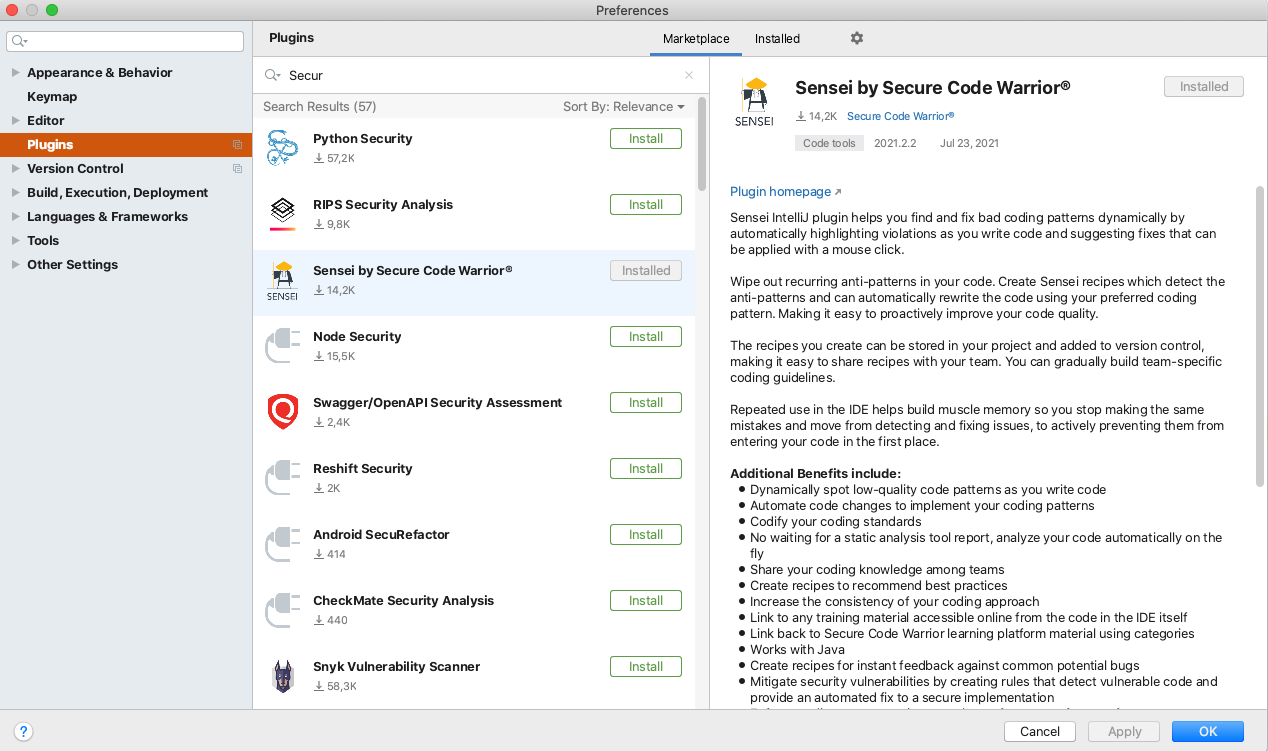
\includegraphics[width=\textwidth]{pluginsmenu.png}
  \includegraphics[width=\textwidth,page=2]{04-tools/figures/figures2.pdf}
  \caption[IntelliJ IDEA Plugins menu]{The Plugins menu in the IntelliJ IDEA allows developers to browse and easily install and uninstall extensions to their IDE.}
  \label{fig:pluginsmenu} 
\end{figure}

Sensei is available in the JetBrains Marketplace and can be installed through this Plugins menu.
Customized versions of Sensei can also be installed through this menu.
Such customized versions might be useful to disable certain features, or to automatically include certain rule sets.
To install customized versions, the Plugins menu needs to be configured to use additional plugin repositories, as shown in Figure~\ref{fig:pluginrepos}.
In this menu the developer needs to add a \gls{url} to locate the Sensei version that should be installed.
The customized version will then show up in the list of plugins in the regular menu.
This installation process is used in an experiment as described in Section~\ref{sec:experiment}.

\begin{figure}
  \centering
  %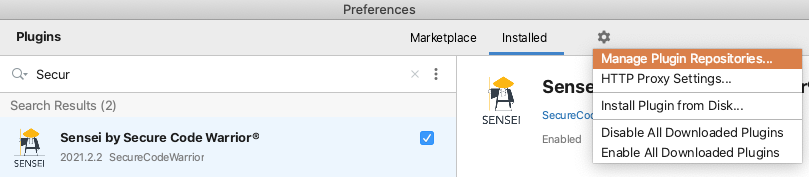
\includegraphics[width=\textwidth]{pluginrepos.png}
  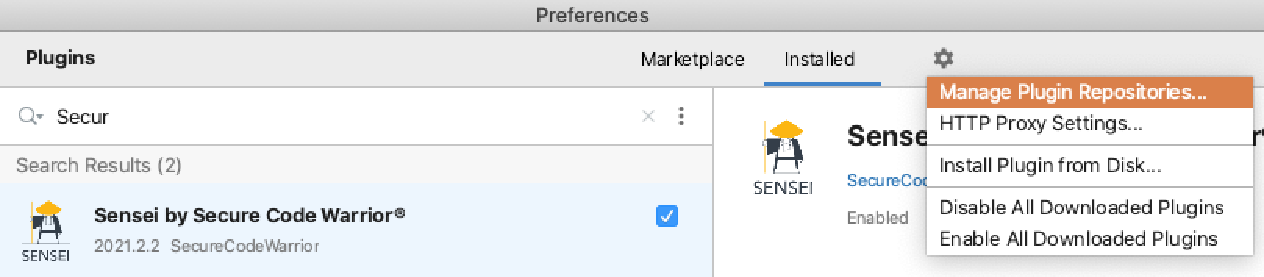
\includegraphics[width=\textwidth,page=1]{04-tools/figures/figures2.pdf}
  \caption[Adding plugin repositories to the Plugins menu]{The Plugins menu can be configured to add additional repositories of plugins, this allows us to install custom versions of the Sensei plugin that should not be distributed publicly.}
  \label{fig:pluginrepos} 
\end{figure}
\section{Recipes}

The \gls{api}-level rules that are enforced by Sensei are called recipes.
This name is chosen to emphasize the difference between Sensei and existing, traditional security tools, which often use rules to scan for vulnerabilities.
Recipes are also commonly used in the \gls{devops} movement, for example by the popular automation tool Chef~\footnote{\url{https://www.chef.io/}}.

\subsection{Creating recipes}
Customization and distribution of the recipes is a crucial feature for any successful tool supporting the paved path methodology.
If the recipes are easy to customize, Sensei can be more easily tuned to provide highly relevant and applicable feedback to the developer.
This customization should be scalable and hence not be a service provided by engineers or experts at \gls{scw}.
It should allow developers and security experts to effortlessly share project-specific or team-specific guidelines among each other.
For this reason, the recipe creation process should be easy and fast, and at the same time versatile. 

Our first approach allowed users to create new recipes through predefined recipe models.
A \gls{gui} was used to let the recipe-writer fill in a number of variables for this model.
A simple example of such a model is  the ``Replace method call model”.
Figure~\ref{fig:recipeedit2} shows a recipe being created to replace the \texttt{addCookie} method with a safe alternative from the \gls{owasp} \gls{esapi}, an open-source, web application security control library designed to make secure development easier~\cite{ESAPI}; the organization also provides some commonly used security guidelines.
The recipe-writer has to fill in some specifics about the method they want to be marked by Sensei, such as the package, class, and method names.
Then they can write one or more quick-fixes.
To create quick-fix, they have to write a quick-fix description and they have to define the code fragment that will be used to replace the original.
For the replacement code, they can reuse arguments, method names, and more from the original code by means of a template language.
In the field ``Rewrite to", the example quick-fix reuses the first argument of the original method call by using the template \texttt{arguments.0}. 

\begin{figure}
  \centering
  %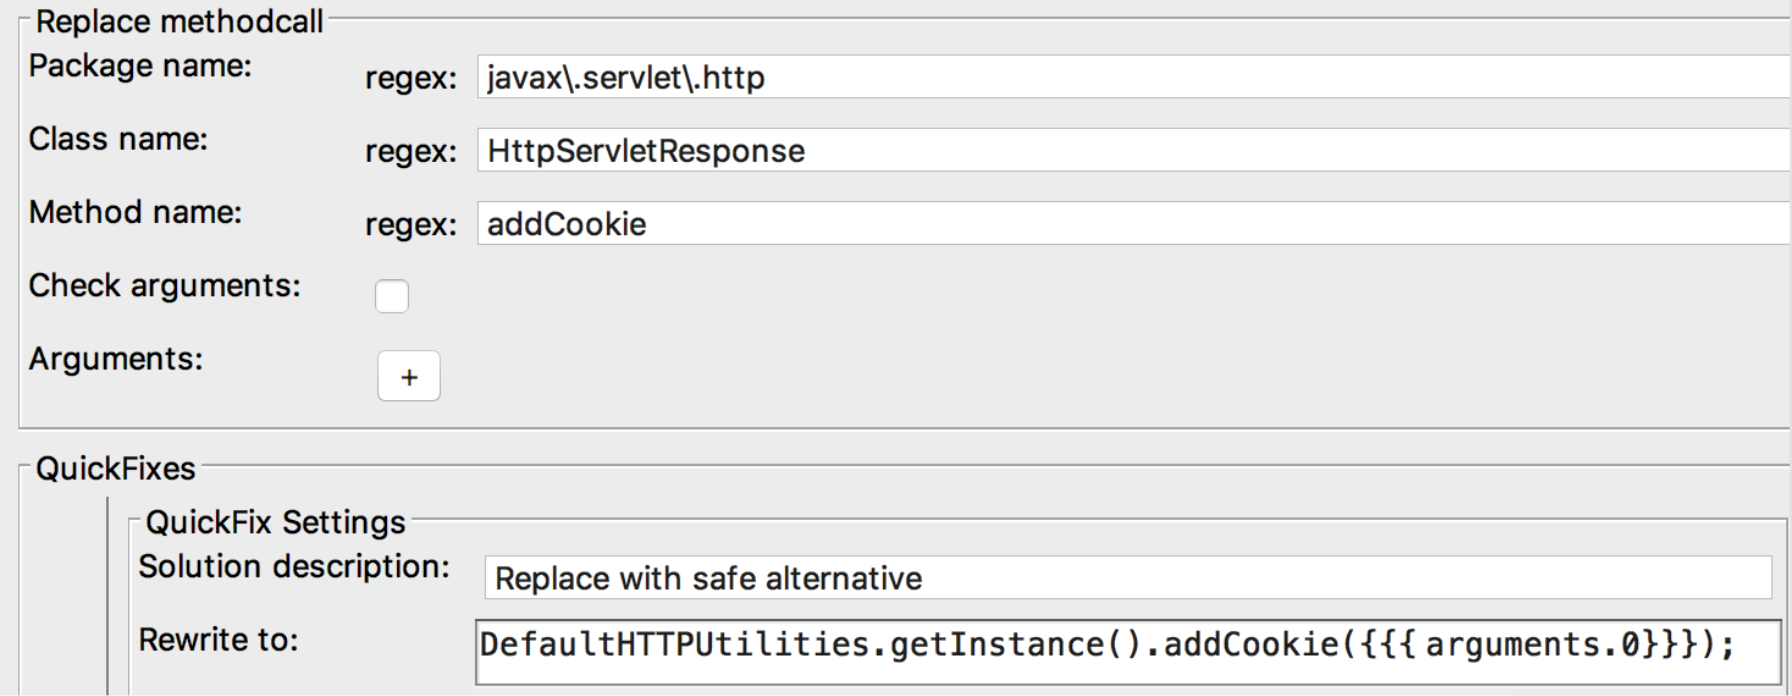
\includegraphics[width=\textwidth]{ruleedit2.png}
  \includegraphics[width=\textwidth,page=7]{04-tools/figures/figures2.pdf}
  \caption[Old model-based recipe editor]{The old recipe editor used a \gls{gui}. It required the recipe-writer to fill in a number of input fields to specify the behaviour of the recipe.}
  \label{fig:recipeedit2} 
\end{figure}

However, for more complex models the number of input fields grew rapidly to accommodate a plethora of corner cases, and so did the number of models for multiple scenarios.
As of now the old recipe editor has over 40 different models.
With this many models, it becomes overwhelming for recipe-writers that have to select a model to enforce their desired coding guideline.
The described model-based recipe creation process is not flexible and intuitive enough, so in the next iteration Nathan Desmet and I designed a new approach.

In this approach we split up the recipe in two parts: A trigger to identify the violation, plus an optional quick-fix to correct the vulnerability consistently according to company best practices.
Triggers are now specified by way of \gls{yaml}\footnote{\url{https://yaml.org/}} syntax, which provides more flexibility.
To develop this \gls{yaml} syntax, all existing Sensei rules were analyzed and grouped based on which elements in the code are incorrect and which transformations are required to fix them.
The resulting taxonomy of 10 bad code patterns is included in Appendix~\ref{app:patterns}.

Since this approach requires recipe-writers to learn the new syntax, we have provided some tools to assist them, in the form of a \gls{gui} that can be used to build the desired recipe from scratch.
In addition, the recipe editor is now more context-aware.
The recipe-writer can open a recipe creation wizard by pressing a key combination in the text editor in the \gls{ide} and selecting ``create new recipe".
This opens a context-aware menu depending on the position of the caret.
For example, if the caret was on a method call, the menu contains an option to create a new recipe that searches for similar method calls, as shown in Figure~\ref{fig:newrecipemethodcall}.

\begin{figure}[t]
  \centering
  %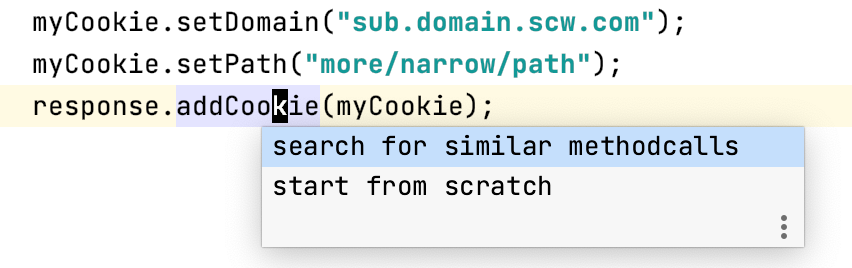
\includegraphics[width=0.8\textwidth]{rulewizard2.png}
  \includegraphics[width=0.8\textwidth,page=11]{04-tools/figures/figures2.pdf}
  \caption[Context-aware recipe creation menu]{The recipe creation menu is context aware, its options will change based on the caret position.}
  \label{fig:newrecipemethodcall} 
\end{figure}

When this context-aware option is chosen, the recipe creation wizard is opened and a recipe is automatically suggested from the available context.
To search for a methodcall, the information that can be pre-filled from context is the type and the name of the methodcall, as well as the number of arguments and each of their types.
The user can then adjust the recipe to reach the desired results through the \gls{yaml} code or the provided \gls{gui}.
This window also provides a preview panel, as shown in Figure~\ref{fig:recipewizard1}.
In this panel, the code file from which the recipe wizard was opened is shown, and the effects of the recipe being created are visualised, which allows for easy customization.

\begin{sidewaysfigure}
  \centering
  %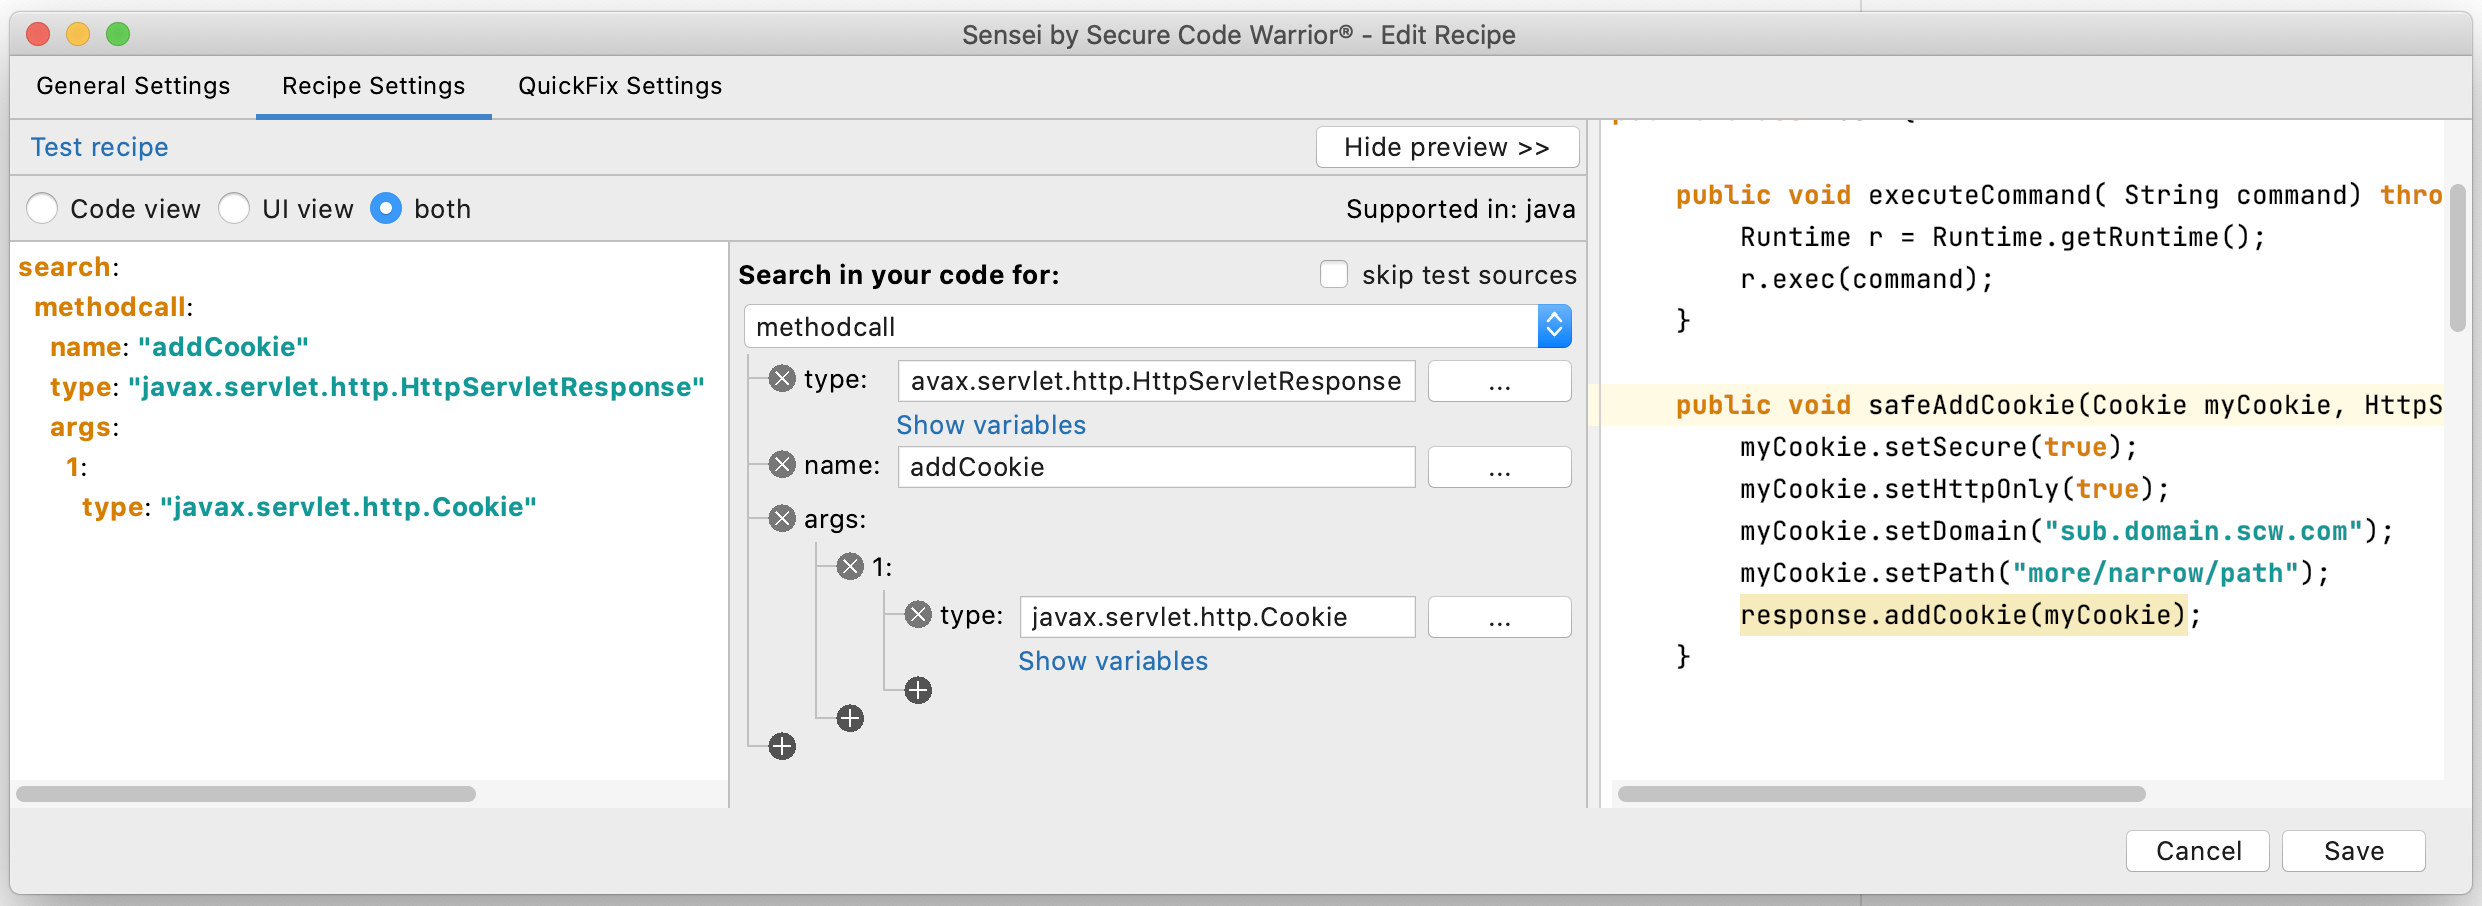
\includegraphics[width=\textwidth]{rulewizard1.png}
  \includegraphics[width=\textwidth,page=10]{04-tools/figures/figures2.pdf}
  \caption[Recipe created from context]{A recipe created through the ``search for similar methodcalls" option in the context-aware recipe creation menu will generate a \gls{yaml}-based recipe with details from the context of the caret position.}
  \label{fig:recipewizard1} 
\end{sidewaysfigure}

After creating a trigger, it is possible to create an optional quick-fix.
Here, the recipe-writer has to fill in the quick-fix description and the replacement code.
For the replacement code, they can make use of the same template language as in the first approach to reuse parts of the original code.
Below the input field, an overview is provided of the available parts of the original code, as shown in Figure~\ref{fig:createfix}.
Double clicking one of these options, adds its template to the fix.
The quick-fix creation window also offers a live preview in the lower right corner that highlights the changes that would be made to the original code (shown in the lower left corner) if the quick-fix is applied.

\begin{figure}
  \centering
  %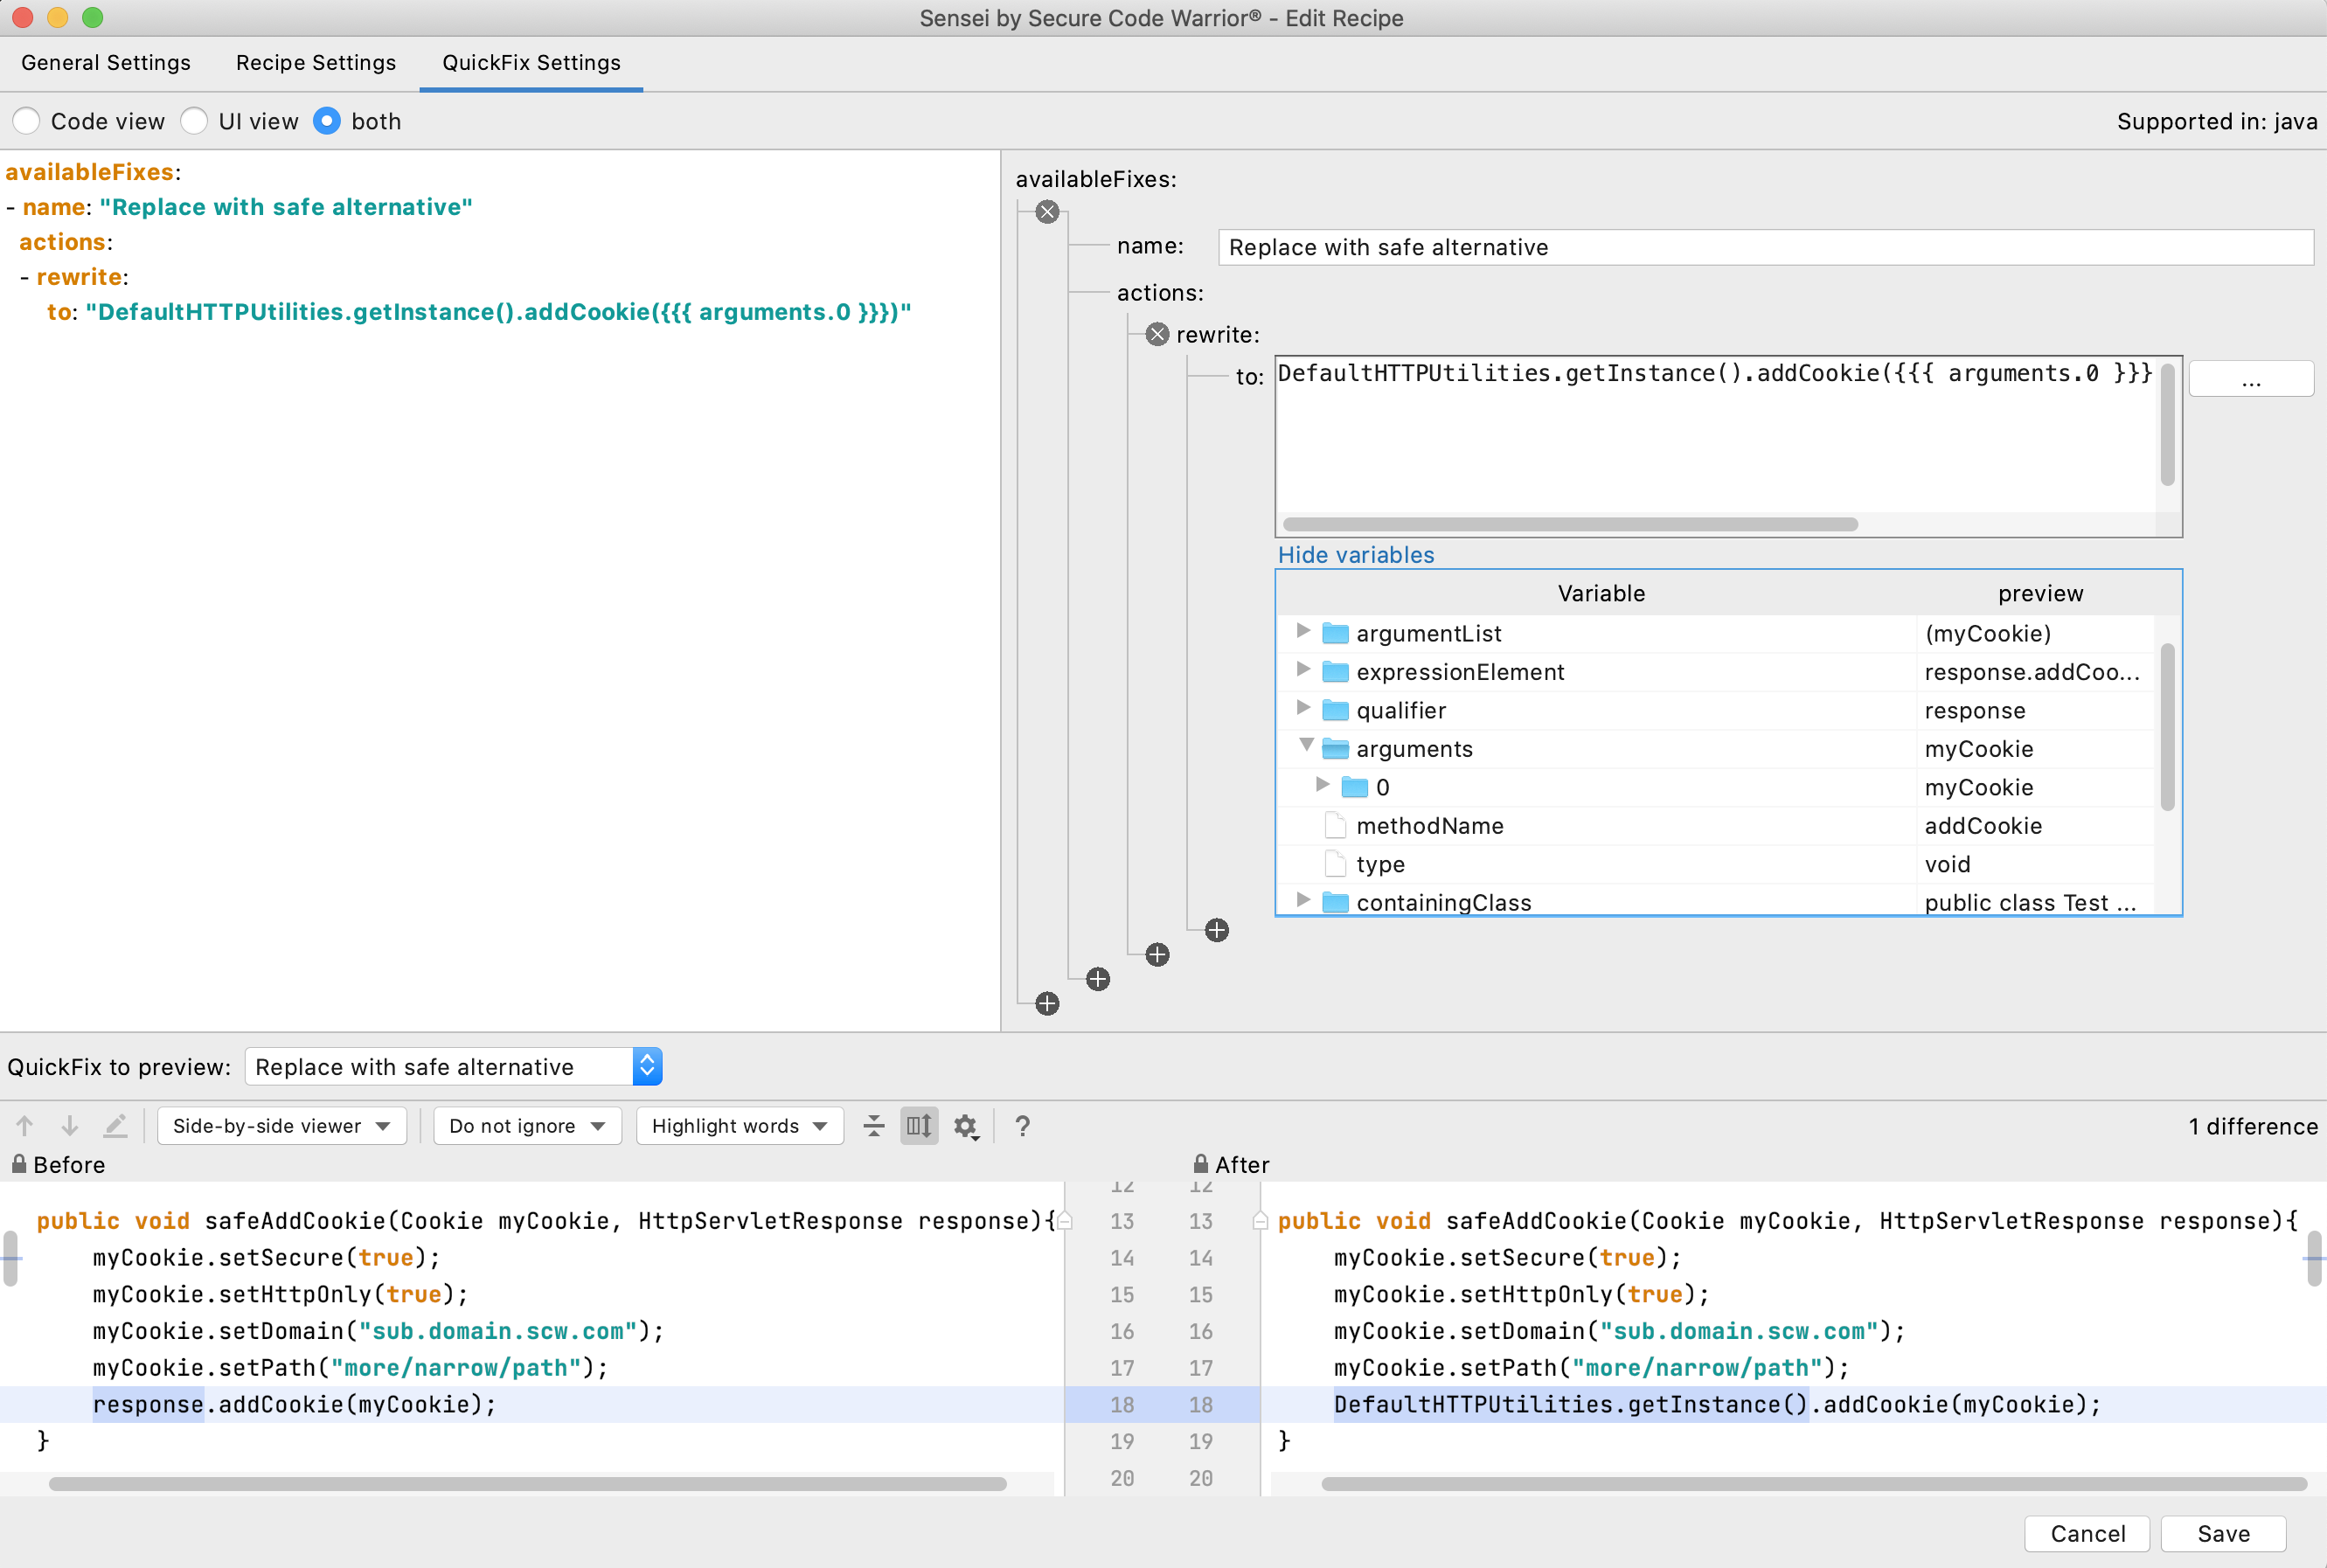
\includegraphics[width=\textwidth]{createfix.png}
  \includegraphics[width=\textwidth,page=5]{04-tools/figures/figures1.pdf}
  \caption[Fix creation window]{The fix creation window allows the recipe-writer to reuse parts of the original code.}
  \label{fig:createfix} 
\end{figure}

Finally, besides the trigger and the fix, there are also a number of general settings for the recipe that can be configured, as shown in Figure~\ref{fig:generalsettings}.
Some examples are the name, descriptions, the category of a related vulnerability, overriding recipes, and scopes.
All of these features are related to the usability of the developer and will be discussed in the following sections.

\begin{figure}
  \centering
  %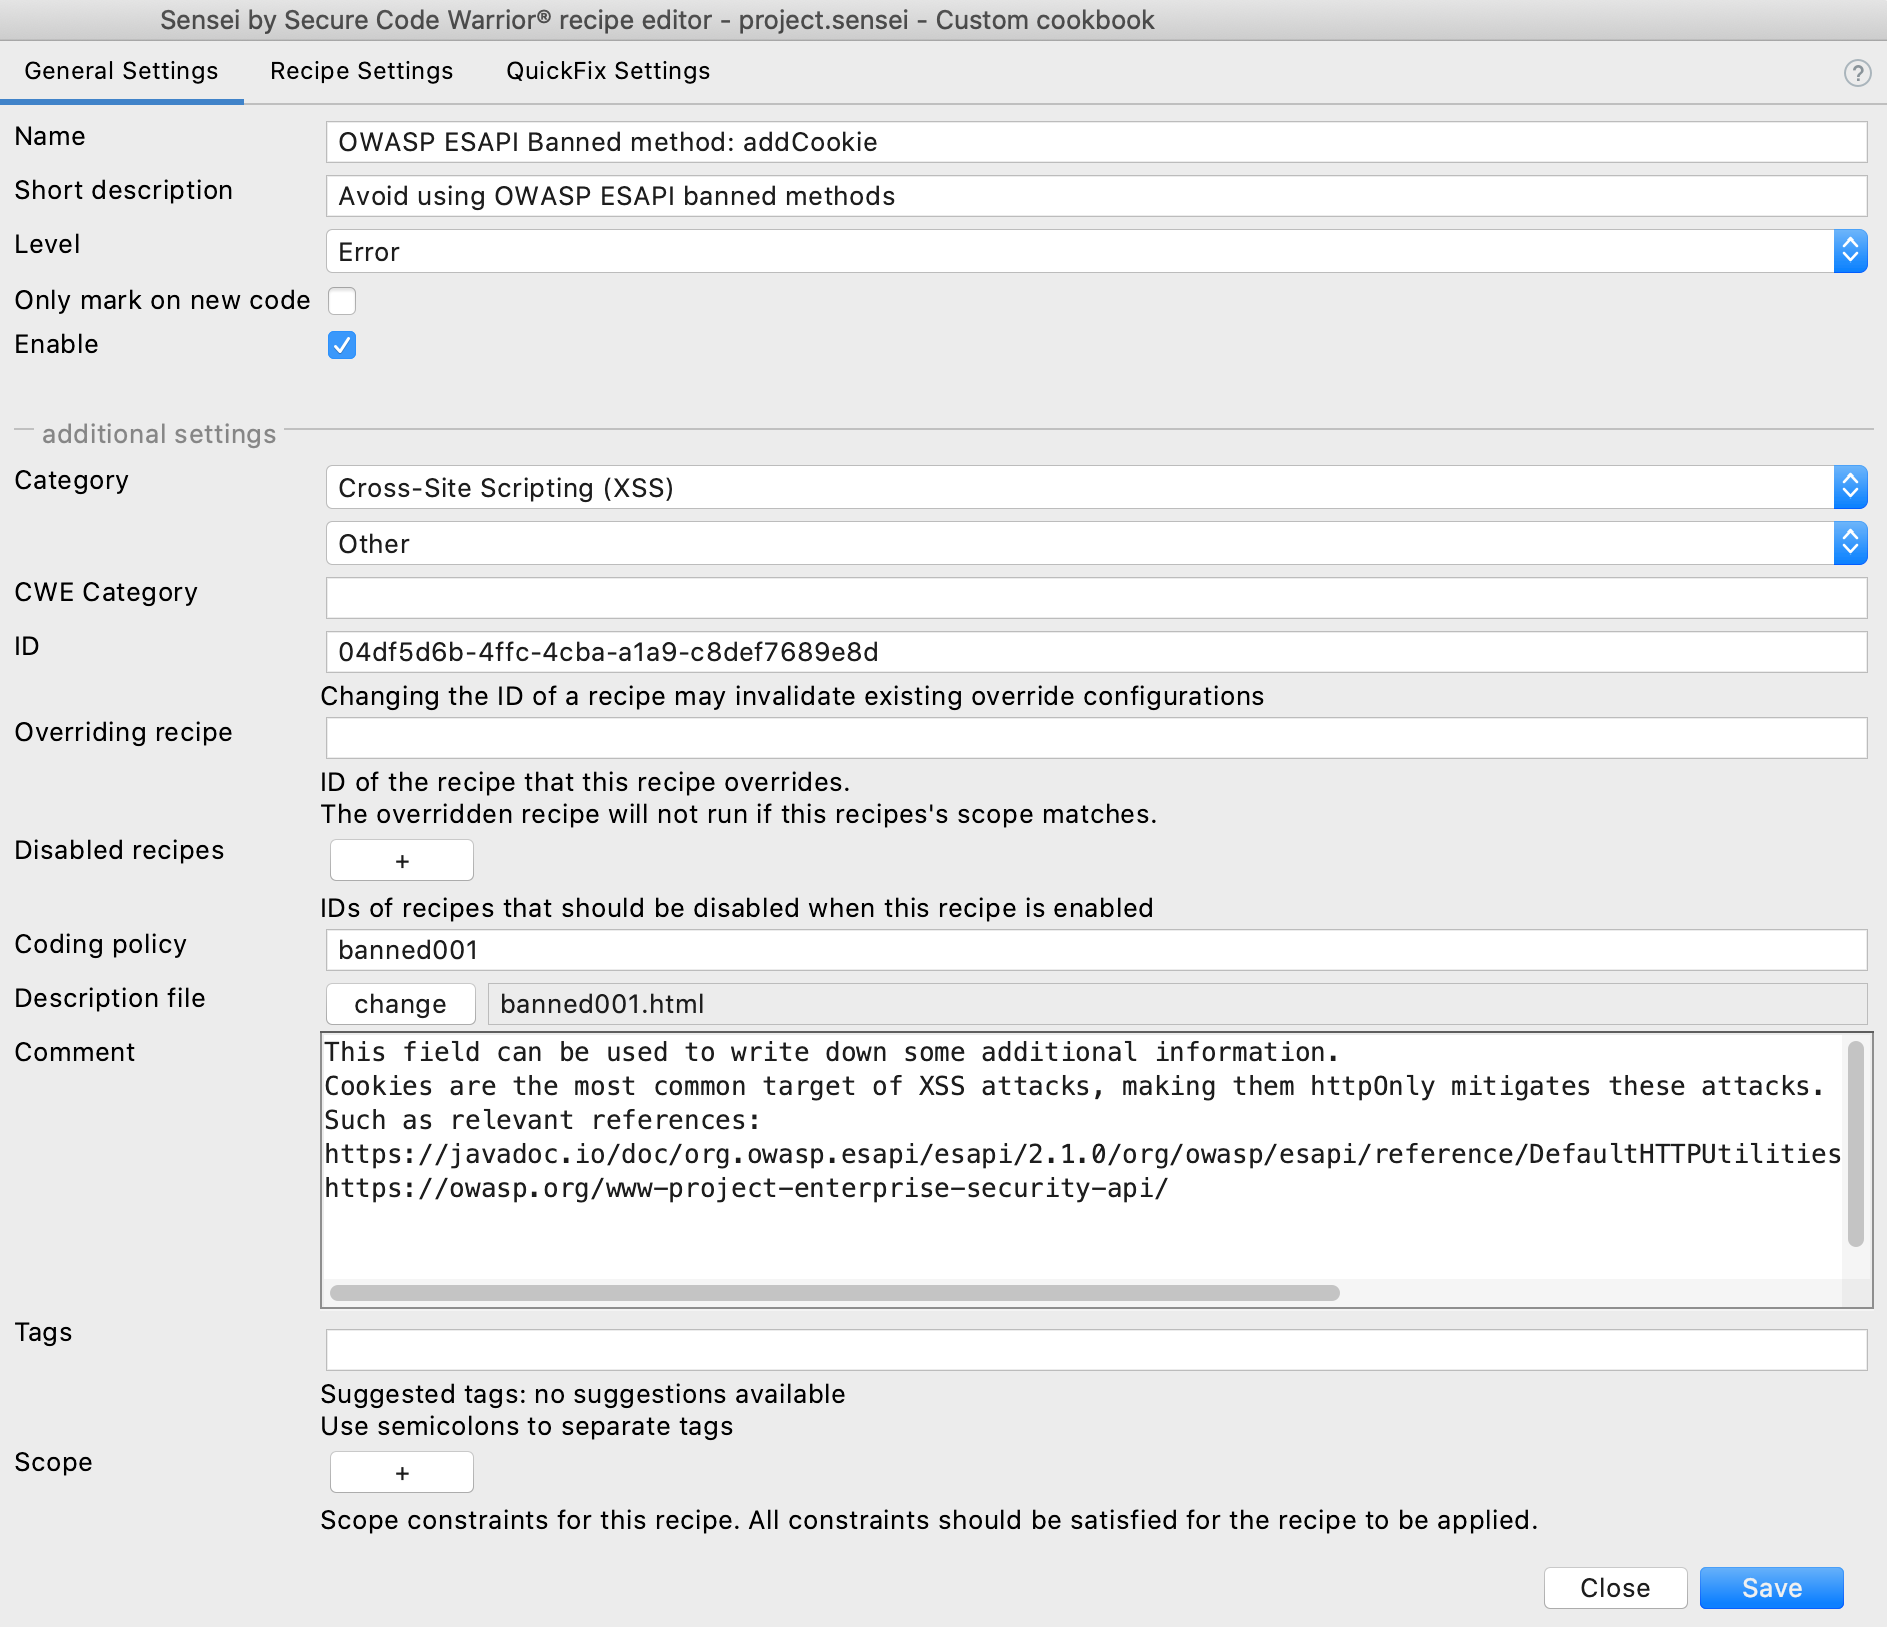
\includegraphics[width=\textwidth]{rulegeneral.png}
  \includegraphics[width=\textwidth,page=8]{04-tools/figures/figures2.pdf}
  \caption[General recipe settings]{Some additional settings are available in the recipe editor mostly related to usability of the developer.}
  \label{fig:generalsettings} 
\end{figure}

When creating recipes in-house, we have observed that the context-aware recipe wizard has greatly sped up the recipe creation process.
In practice, creating new recipes often starts from a bad code example, either when fixing a vulnerability or while reviewing the code of a colleague.
The recipe-writer can then simply open the recipe creation wizard from this example.
The live previews also greatly improve the usability, since before they were introduced, to create a finished recipe the recipe-writer was required to go back and forth several times to test the recipe in the \gls{ide} and adjust it in the recipe editor.



\subsection{Managing recipes}
\label{sec:manager}
%\todo[inline]{could you please explain how a developer would know where to consult for recipe sets, depending on which APIs are being used in a program? Bjorn: Mijn originele vraag is nog steeds geldig: Waarom denk je hier niet explicieter op te antwoorden? De vraag is volgens mij hoe developers de sets kunnen consulteren, hoe ze weten welke sets voor hen toepasbaar zijn. De vraag van de reviewer was niet hoe de regels tot stand komen.}
In the paved path methodology, guidelines can be put in place at the start of the project.
If not, at the very least, relevant guidelines should be created each time a new feature is going to be developed.
Together with those guidelines, Sensei recipes should be created as well.
The recipes, however, can also be used by the developers themselves, as a way to share knowledge.
When they develop new \glspl{api}, additionally to documentation, developers can also add Sensei recipes to the project that help their colleagues use these \glspl{api} as intended.

We also recommend to make Sensei recipes part of the remediation process when problems are found by security testing or reported through bug bounty programs.
It should be part of the process to create a recipe that prevents this same vulnerability from occurring in the future.
Currently, it is often the case that security experts run the security scans.
When problems are found, these experts guide the developers by providing them with informal, broadly applicable guidelines and checklists.
These instructions sometimes use security jargon that might not be clear to all developers, and even if they are understood, that does not guarantee the developer will be able to apply them in practice.
In the paved path methodology, security experts and developers should work together to create \gls{api}-level guidelines instead.
As part of this process, to communicate these guidelines to the rest of the team, Sensei recipes can be created as well.

For existing projects, we recommend companies to start with no recipes and use existing data on the security of their project as a starting point.
This could be the report of a penetration test, or results of vulnerability scans.
While resolving these issues in the code, developers and security experts can start building the first recipes.
Some clients of \gls{scw} have been hesitant to start with an empty security tool and, despite our recommendations to customize recipes for each project, still wish to receive starting recipes.
For this reason we have created small open-source sets of unopinionated recipes that can be used in all projects\footnote{\url{https://securecodewarrior.github.io/public-cookbooks/}}.
These recipes aid in correctly using the standard libraries of certain popular frameworks (e.g., Java 
\gls{ee}, Android \gls{sdk}, \gls{aws} \gls{sdk}).
This set can be used as inspiration and to get both security experts and developers accustomed to the tool, but usually it does not flag many issues.

Considering the different sources of recipes, developers can have recipes imposed by management and/or by the security team, as well as recipes distributed among the developers per team or project.
On top, there is the open-source recipes that can be used as a starting point when first using the tool.
To make the management of recipes easier, we group recipes into cookbooks.
Instead of distributing recipes one-by-one, this allows for grouping and distributing related recipes more easily. 

In order to manage these cookbooks in the \gls{ide}, a cookbook manager is provided, as shown in Figure~\ref{fig:cookbookmanager}.
Each cookbook is specified by a name and a location.
The developer can enable or disable any cookbook as well as edit recipes in some cookbooks.

\begin{figure}
  \centering
  %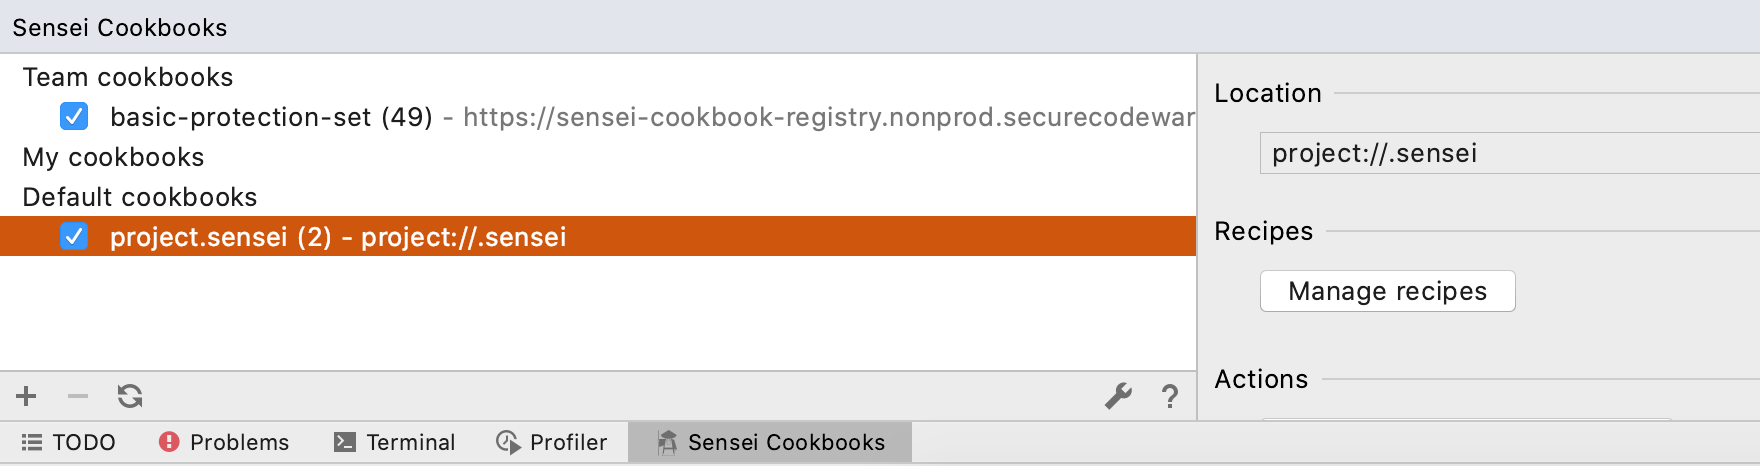
\includegraphics[width=\textwidth]{cookbookmanager.png}
  \includegraphics[width=\textwidth,page=3]{04-tools/figures/figures1.pdf}
  \caption[Cookbook manager]{The cookbook manager in this screenshot contains one remote team cookbook as well as one default cookbook stored in the project structure.}
  \label{fig:cookbookmanager} 
\end{figure}

Cookbooks can be stored locally or remotely.
Remote cookbooks are called team cookbooks and can be loaded from a github project (e.g., \texttt{git@gitserver:cookbooks|master|recipes}) or another remote server location (e.g., \texttt{https://remote.com/recipes.zip}).
Remote cookbooks are only recommended to distribute generally applicable cookbooks, since remote recipes are not editable by the developers and are instead read-only.
Any updates to the remote cookbooks are automatically pushed to all the developers.
Locally stored cookbooks are editable and can be specified by a local path (e.g., \texttt{/Users/dev/recipes}) for personal cookbooks or a path starting from the project root (by default \texttt{project://.sensei}) for default cookbooks for a project.
Local cookbooks are editable which means they can also be enabled on a recipe-by-recipe basis.
It is advised to store project specific recipes as part of the project.
This way, the recipes are always available, up-to-date with the code, and following the same flow as regular code (e.g., branch, review, merge).
When recipes follow the same flow as the code, new \glspl{api} and the recipes needed to use them properly can be added to the project and reviewed as a whole. 

The paved path methodology encourages customization of the recipes at project level.
Previous research and experience have shown that customization at at this level is the most successful.
This provides the needed flexibility to tailor the enforced coding guidelines to the code, but also ensures that the team has a joint approach to how the code for a project should be developed~\cite{sadowski2015tricorder}.
Individually customized recipes might lead to disagreements, while company-wide recipes might be too general to be easily applied.

It is possible for a recipe to be configured to disable other recipes, as shown in the general settings in Figure~\ref{fig:generalsettings}.
This feature can be used to improve remote, read-only recipes.
It is possible that such a recipe is not fully applicable to the project, e.g., because it requires too many manual adaptations.
It is then possible to create a replacement recipe that can be distributed to one team or project and disables the original recipe when it is active.
To facilitate this, an option in the quick-fix menu is added to copy remote recipes to a local cookbook, as shown in Figure~\ref{fig:copyrecipe}.
This option can easily be hidden in the settings.
The clone recipe window, shown in Figure~\ref{fig:clonewindow}, provides an option to automatically disable the original recipe it is copied from.
When a remote recipe is disabled or replaced, the author of this recipe should be notified.
It is possible that it is a generally applicable improvement and the recipe can be updated accordingly for other teams or projects that use it in a remote cookbook.
An additional quick-fix option will be added in the future to disable a recipe.

\begin{figure}
  \centering
  %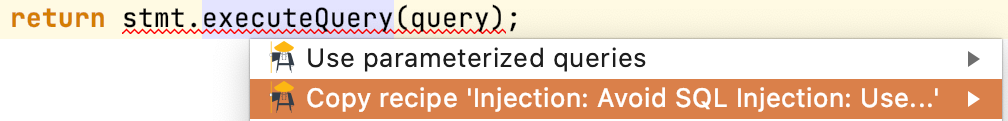
\includegraphics[width=\textwidth]{copyrecipe.png}
  \includegraphics[width=0.9\textwidth,page=4]{04-tools/figures/figures1.pdf}
  \caption[Copy recipe option in the quick-fix menu]{For remote recipes, the quick-fix menu offers a ``Copy recipe" option.}
  \label{fig:copyrecipe} 
\end{figure}

\begin{figure}
  \centering
  %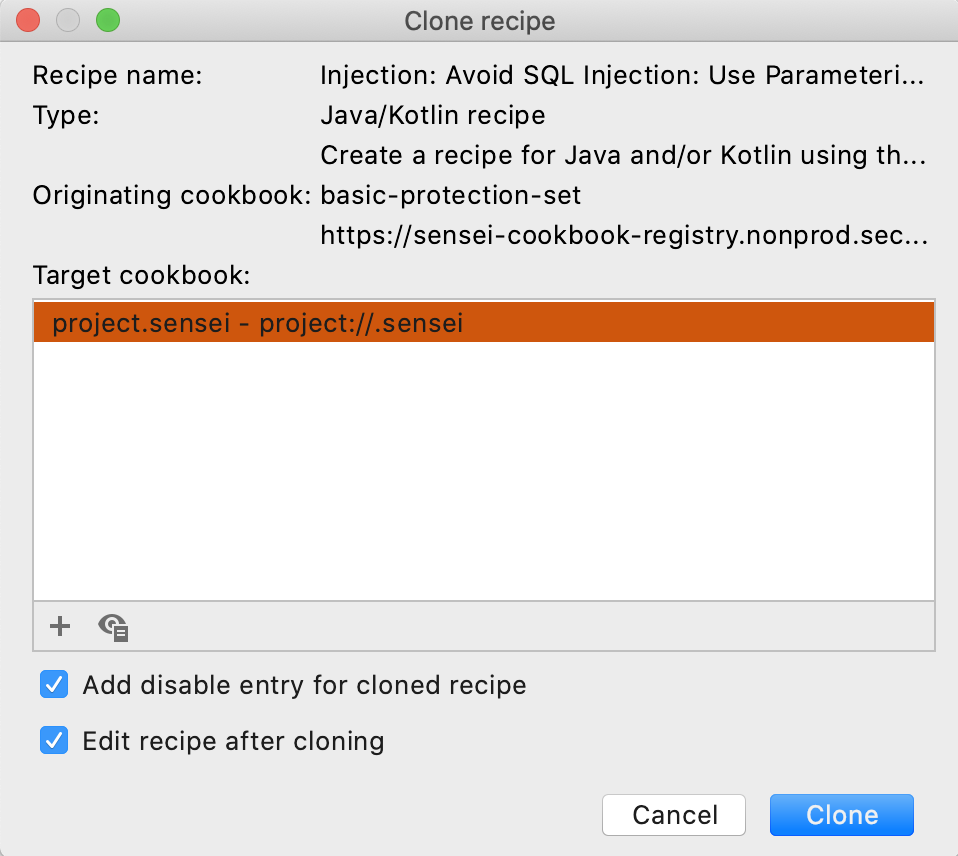
\includegraphics[width=0.75\textwidth]{clonerecipe.png}
  \includegraphics[width=0.75\textwidth,page=2]{04-tools/figures/figures1.pdf}
  \caption[Clone recipe window]{The clone recipe window allows the recipe-writer to configure the new recipe to disable the recipe it is copied from.}
  \label{fig:clonewindow} 
\end{figure}

The discussed features to disable recipes have been designed to improve the usability of the tool for developers.
They are in line with the philosophy that developers' productivity benefits from their ability to customize their development environment to their preferences, and to give them a significant amount of freedom in that regard.
In that philosophy, it is preferable to have developers disable some recipes rather then uninstalling or neglecting the tool completely.
Importantly, this does not necessarily result in guideline violations slipping below the radar, since security and management can still have these recipes, as well as complimentary tools, enabled in later phases of the \gls{sdlc}.

\subsection{Verifying recipes}
To inspect the code against a number of recipes, our tool reuses the \gls{ide} syntax checking features.
When a developer writes new code, the \gls{ide} rebuilds the \gls{ast} and computes the changes compared to the previous version.
A limited \gls{ast} of the changes, containing the necessary symbol information, is then passed on, allowing tools to only analyze the changes.
On this \gls{ast}, a combination of specialized light-weight versions of existing analysis techniques is used such as taint analysis, data flow analysis, and control flow analysis to verify the recipes in real time.

\subsection{Explaining recipes}
\label{sec:information}
In order to mark violated guidelines, our plugin makes use of existing \gls{ide} features to flag coding mistakes.
In most \glspl{ide} the code markings by default have three levels of severity: \emph{error}, \emph{warning}, and \emph{information}.
We recommend to mark coding guideline violations as errors.
Traditional error-level markings are usually immediately addressed by the developer, while warning-level markings are more frequently ignored~\cite{whitney2018embedding}.
This is the case because error-level warnings in an \gls{ide} typically indicate a problem in the code that will result in a compilation failure.
Currently error markings by our tool still allow successful compilation of a project, but several clients have requested for the markings to result in compilation failures, equivalent to errors marked by the \gls{ide} itself.
This is not surprising, as it is in line with the default behavior of popular \glspl{ide} such as Visual Studio.
For example, when Visual Studio's C compiler compiles code that uses the insecure \texttt{sprintf} function, it throws a compilation error warning the developer that the function may be unsafe.

An example marking can be seen in Figure~\ref{fig:publicactivity}, where the opening \texttt{<activity>} tag in \gls{xml} code is marked as an error.
This marking makes the code fragment stand out and attracts the developer's attention.
In the example, the Android activity is configured as a public activity by setting the \texttt{exported} attribute to \texttt{true} but not configuring an intent filter.
In \gls{xml} code, like in this example, it is advised to only mark the opening tag, and not the entire \gls{xml} tag and its content.
This would overwhelm the developer, and it would not be clear which part of the code is lacking. 

\begin{figure}
  \centering
  %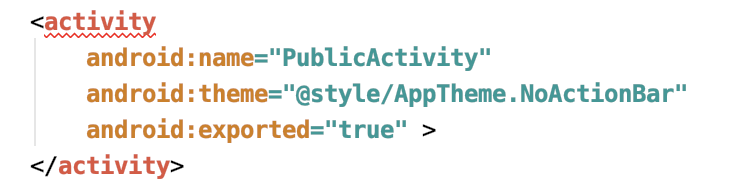
\includegraphics[width=.75\linewidth]{publicactivity.png}
  \includegraphics[width=0.75\textwidth,page=3]{04-tools/figures/figures2.pdf}
  \caption[Error marking on an XML opening tag.]{\Gls{xml} recipes can be configured to mark the opening tag only (shown in the figure), the opening tag and the closing tag, or both tags and their entire content.}
  \label{fig:publicactivity} 
\end{figure}

Permanent markings, that remind developers of security implications of their decisions, should be marked as information.
To continue on the example of private and public activities, in the code file that implements the activity, we mark the class definition at the information level.
Hovering over the marking informs the developer whether the activity is configured as public or private, and provides a direct link to detailed information about the security implications.
This marking is shown in Figure~\ref{fig:infomarking}.
Note how the markings are clearly visible and noticeable, but at the same time non-intrusive to developers already used to their \gls{ide} flagging code fragments.

\begin{figure}
  \centering
  %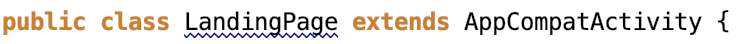
\includegraphics[width=0.80\linewidth]{infomarking2.png}
  \includegraphics[width=0.8\textwidth,page=10]{04-tools/figures/figures1.pdf}
  \caption[Marking at the information error level]{The information error level marking is clearly visible but at the same time non-intrusive, as this is a permanent marking that can not be resolved.}
  \label{fig:infomarking} 
\end{figure}

The marking of code is accompanied by three descriptions.
The information in these descriptions is important to ensure the continued use of the tool~\cite{whitney2018embedding,layman2007toward}.
Developers build trust with analysis tools, and this trust is quickly lost if they do not understand the tool’s output~\cite{bessey2010few}.
The first description is the short error description, i.e., the text that appears when the developer hovers their mouse pointer over the marked code.
It should be just one line.
The purpose of this description is to attract attention, inform the developer that something should be addressed, not to explain how to address it.

We have learned through user feedback that it is most effective to attract the user's attention by starting with the “why”~\cite{RSAvideo}, the reason the code is marked and should be addressed.
In the past the short description used to indicate the possible vulnerability class, for example “Could lead to SQL injection”. 
We believed that starting with the potential consequences, makes the developers realize the severity of their mistake and encourages them to immediately address it.
However, as explained in Section~\ref{sec:communication}, security jargon should be avoided when communicating to developers.
The feedback in all of the descriptions should be targeted at developers, and hence the focus should be on the guidelines that were put in place, on the paved path.
A better short description is hence, “Violates a guideline on data retrieval”, as depicted in Figure~\ref{fig:shortdescription}.

\begin{figure}
  \centering
  %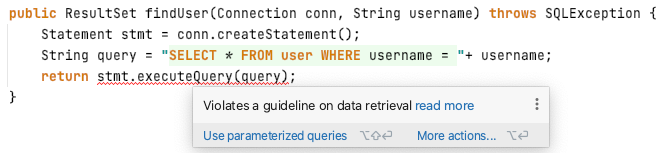
\includegraphics[width=\linewidth]{shortdescription2.png}
  \includegraphics[width=\textwidth,page=14]{04-tools/figures/figures2.pdf}
  \caption[Short description of a recipe]{The short description of a recipe is visible when hovering over a marking. It should attract the developers attention but avoid security jargon. Instead, the developer can be reminded of guidelines that are in place.}
  \label{fig:shortdescription} 
\end{figure}

Next to the short description a “read more” link is created by the \gls{ide} for the interested developer.
Upon clicking this link, a pop-up is opened to show a more elaborate \gls{html} page.
This is the second description.
Figure~\ref{fig:fulldescription} shows an example.
This description is called the full coding guideline.
The page starts with a short abstract, stating in one sentence what should be done, such as “Secure coding practices prescribe that queries need to be parameterized”.
The page's next section presents in detail what it means to use parameterized queries and gives an overview of the approved \gls{api} methods.
Small code examples are included as well, since previous research has shown examples are the fastest way for developers to understand a problem~\cite{whitney2018embedding}.
The goal of this description is after all to help developers find out quickly how to comply to the coding guideline without spending much time or effort.
This is crucial for a security tool to feel well integrated into developer workflows.
The last section of the description contains a list of possible consequences when the developer fails to address this issue.
There is no mention of vulnerabilities or exploits until this point.
Each item in the list contains a link to the \gls{scw} training platform to learn more about the vulnerabilities and how they are exploited.
This way an interested developer (with too much time on their hands?) can still easily find the necessary information to learn the details of each vulnerability and the possible attacks.
Following this training would require a context switch and would likely hurt developer productivity.
In the future the integration between the \gls{scw} training platform and the Sensei \gls{ide} plugin can be improved as described in the perspectives in Section~\ref{sec:its-integration}.

\begin{figure}
  \centering
  %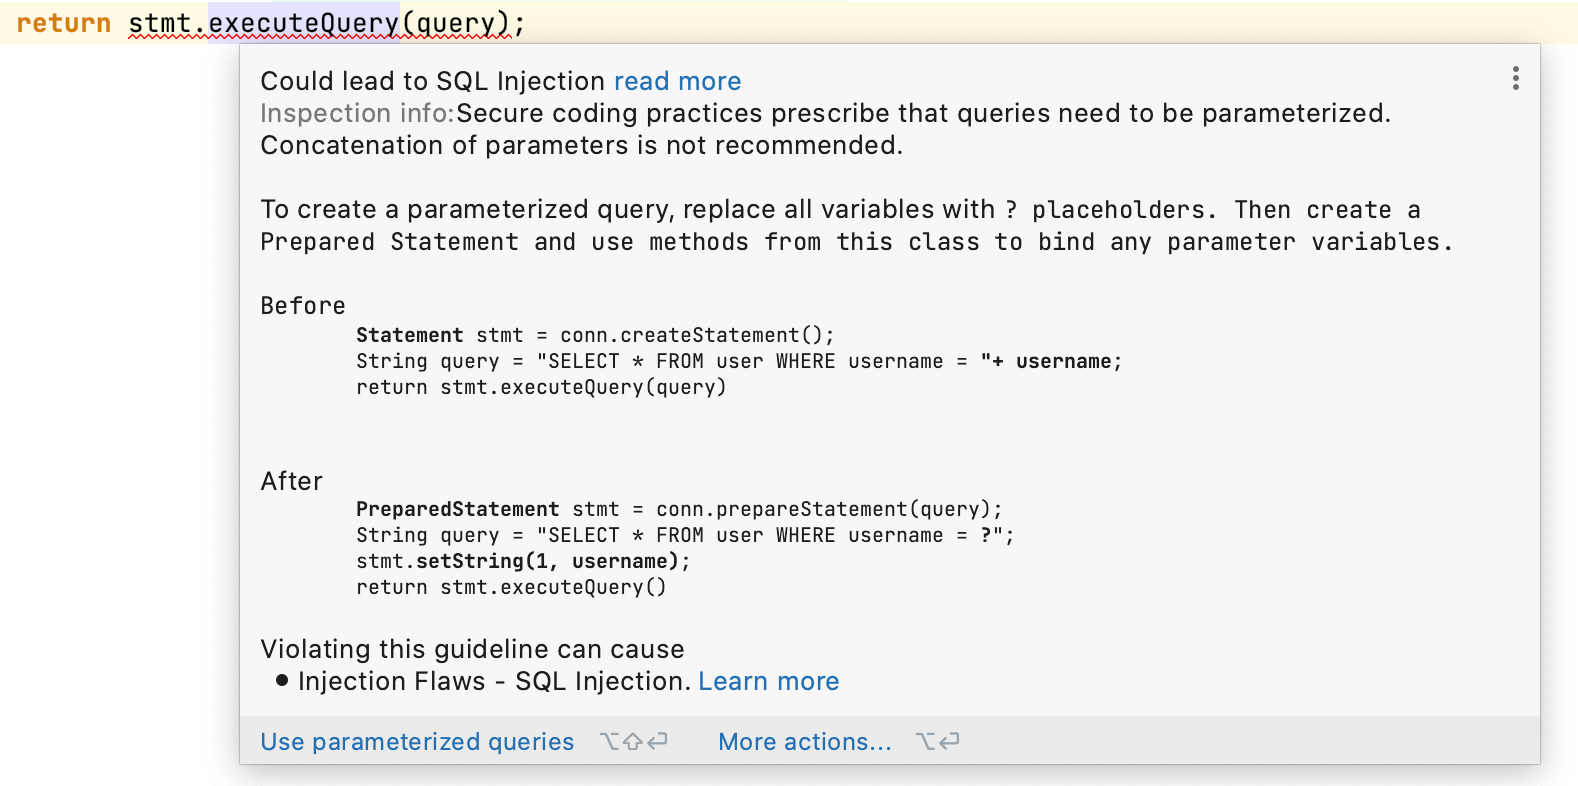
\includegraphics[width=\textwidth]{guideline.png}
  \includegraphics[width=\textwidth,page=7]{04-tools/figures/figures1.pdf}
  \caption[Example of the full coding guideline.]{The full coding guideline is a more elaborate \gls{html} page that explains the guideline in more detail and provides code examples.}
  \label{fig:fulldescription}
\end{figure}

The third description is visible to the developer when they press the \gls{ide}’s key combination to start resolving the issue.
A drop down menu appears, containing the possible quick-fixes' descriptions.
%A "copy recipe" option is available as well, and for local recipes there is also additionally an "edit recipe" option, both of these can be disabled in the Sensei settings.
IntelliJ also provides options to disable inspections locally or globally. Figure~\ref{fig:qfdescription} shows an example.
In this menu we provide a very short description of the actions that will be performed when this code transformation is chosen, such as “Use parameterized queries”.
A brief yet descriptive quick-fix description allows developers to decide quickly whether the fix is appropriate for them.
If the effects of applying the quick-fix are well understood, the developer will trust the tool and apply the fixes more often.
Sometimes the developer needs to choose between different possible solutions.
However, it is advised to keep the number of fixes as low as possible, as to not complicate the issue unnecessarily.

\begin{figure}[t]
  \centering
  %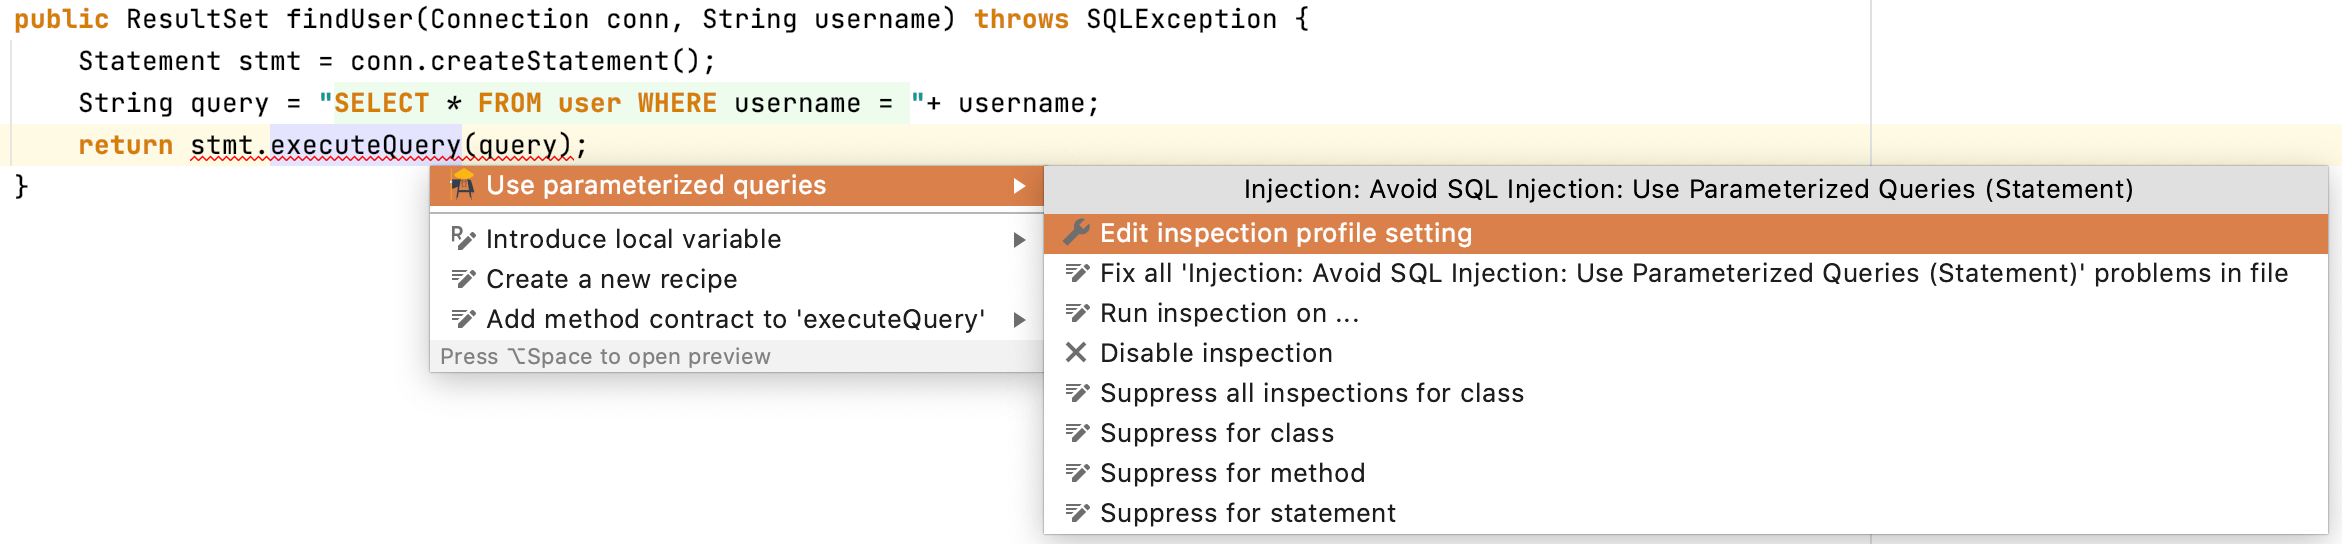
\includegraphics[width=\textwidth]{quickfixmenu.png}
  \includegraphics[width=\textwidth,page=5]{04-tools/figures/figures2.pdf}
  \caption[Example of the quick-fix description.]{The quick-fix description briefly describes the actions that will be performed when each option is chosen. IntelliJ also offers a feature to suppress markings of any inspection (Sensei or otherwise).}
  \label{fig:qfdescription} 
\end{figure}

\section{Recipe features}
\label{sec:features}

Over time, several advanced features in the recipes have been developed following user feedback.
In this section, I explain the problems they tackle and provide code examples for each one.

\subsection{Lowering effective false positives}
\label{sec:efp}
It is important to choose the right error level for the developer to pay attention to the markings, but also not to overwhelm them with markings to the point that they start to ignore them.
Since the recipes can be created by anyone in the team, they should not be too obtrusive.
To a recipe writer, a false positive is an incorrect marking of code that is not violating a coding guideline.
However, to a developer, a false positive is any code marking that they do not intend to fix and ignore instead~\cite{ayewah2007evaluating}.
A false positive from the perspective of the developer is also called an \gls{efp}~\cite{sadowski2015tricorder}.
To ensure the usability of the tool, the \gls{efp} rate should be sufficiently low~\cite{sadowski2015tricorder,johnson2013don}.

To demonstrate \glspl{efp} we take a look at \gls{os} Command injection.
One of the \glspl{api} that is banned in the \gls{owasp} \gls{esapi} guidelines is \texttt{Runtime.exec}.
This \gls{api} is used to execute \gls{os} commands in Java programs.
When user input is added to this command, \gls{os} command injection is possible and the attacker can gain access to the underlying \gls{os}.
Using this information it is possible to create a recipe that marks all uses of the \texttt{Runtime.exec} method.
While this is a good coding guideline, a security conscious developer recognizes that the method needs user input before it can lead to \gls{os} command injection.
In rare occasions an \gls{os} command might be necessary for functionality and perfectly valid and secure.
For example, launching another software product can be done securely as long as the command is hard-coded.
An example of insecure usage of the \texttt{Runtime.exec} method can be found in Listing~\ref{lst:oscommand1}, examples of secure usage in Listings~\ref{lst:oscommand2}~and~\ref{lst:oscommand3}.
The two secure examples are still violations of the above coding guideline, and they get flagged.
An experienced developer has no intent to fix them, meaning they are two cases of \glspl{efp}.
Notice how this \gls{efp} depends on the knowledge and skill of the developer, meaning that it might be beneficial to adjust the feedback of the tool for individual developers, as explained in the perspectives in Section~\ref{sec:sensei-perspectives}.
%A similar example leading to \glspl{efp} is when hard-coded \gls{sql} queries are created without using parameterized queries.
%These queries would violate a guideline enforcing parameterized queries, but they would not be insecure, not even when this function is reused from a different context in the future.

In order to keep the \gls{efp} rate sufficiently low we have introduced the concept of \emph{trusted input}.
Hard-coded input is automatically trusted, since a user can not influence it, and hence it can not lead to a vulnerability.
However, function parameters and variables from other origins are considered untrusted by default.
This is still in line with the philosophy to protect methods from future use, where we want to flag violations that can one day lead to vulnerabilities.
The requirement in recipes of untrusted input can be added to arguments, this can be done using the \gls{yaml} syntax or by using the \gls{gui} as shown in Figure~\ref{fig:recipegui}. 
The next step is to define trusted sources. This also avoids the \gls{efp} in Listing~\ref{lst:oscommand3}. The resulting recipe can be seen in Listing~\ref{lst:yamlrecipe}.

\begin{minipage}[t]{0.9\linewidth}
%\vspace{-0.4 cm}
\begin{lstlisting}[language={Java},caption={if the \texttt{command} variable contains unsanitized user input, this function is vulnerable to \gls{os} command injection.},label={lst:oscommand1},abovecaptionskip=-0.0pt,xleftmargin=15pt]
public void executeCommand(String command){
    Runtime r = Runtime.getRuntime();
    r.exec(command);
}
\end{lstlisting}
%\vspace{-0.3cm}
\begin{lstlisting}[language={Java},caption={Using a hard-coded command avoids the possibility that the variable will ever contain unsanitized user input.},label={lst:oscommand2},abovecaptionskip=-0.0pt,xleftmargin=15pt]
public void executeCommand(){
    Runtime r = Runtime.getRuntime();
    r.exec("explorer.exe");
}
\end{lstlisting}

\begin{lstlisting}[language={Java},caption={This code fragment is secure if the \texttt{getSafeCommand} method can be trusted to never return variables containing unsanitized user input.},label={lst:oscommand3},abovecaptionskip=-0.0pt,xleftmargin=15pt]
public void executeCommand(){
    Runtime r = Runtime.getRuntime();
    String command = getSafeCommand();
    r.exec(command);
}
\end{lstlisting}

\begin{lstlisting}[language={yaml},caption={This recipe trigger requires the argument of an \texttt{exec} methodcall to contain untrusted input before it will mark the methodcall. It also specifies the methodcall \texttt{getSafeCommand} as a trusted source of input.},label={lst:yamlrecipe},xleftmargin=15pt]
search:
  methodcall:
    name: "exec"
    type: "java.lang.Runtime"
    args:
      1:
        type: "java.lang.String"
        containsUntrustedInput: true
        trustedSources:
        - methodcall:
            name: "getSafeCommand"
\end{lstlisting}
\end{minipage}
%\vspace{-.3cm}

\begin{figure}[t]
  \centering
  %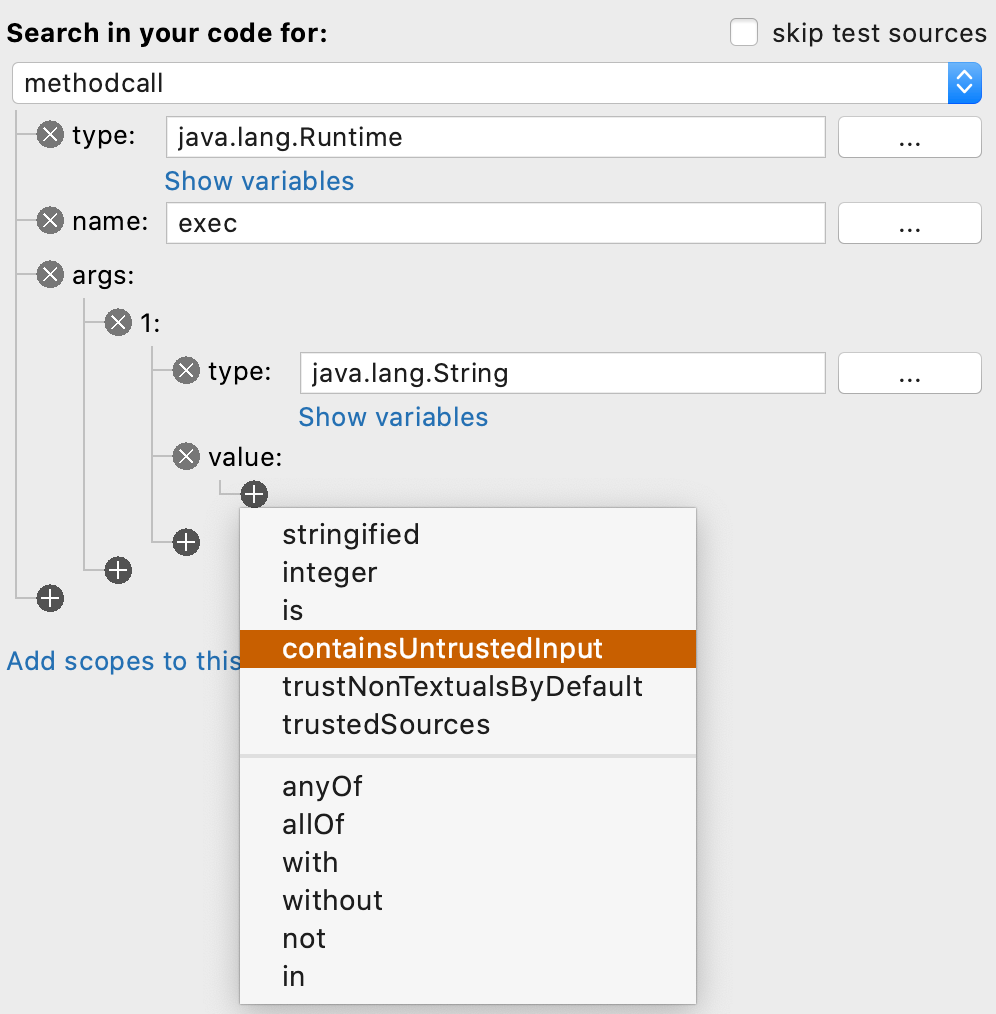
\includegraphics[width=\textwidth]{rulegui2.png}
  \includegraphics[width=\textwidth,page=9]{04-tools/figures/figures2.pdf}
  \caption[\Gls{gui} to add the requirement of untrusted input.]{It is possible to add requirements like untrusted input or an in-clause through the \gls{gui}.}
  \label{fig:recipegui}
\end{figure}

Another way to allow recipe writers to create more targeted recipes and to keep the \gls{efp} rate low, is to provide \emph{trigger scopes}.
Trigger scopes can be added by using the \texttt{in} keyword in the \gls{yaml} syntax, or by using the \gls{gui} as shown in Figure~\ref{fig:recipegui}.
The in-clause can define restraints on the context.
This makes it possible to create a recipe that prevents the usage of \texttt{Runtime.exec} except in a class with name \texttt{AppLauncher}.
Scopes like this can also help with performance, i.e., meeting the real-time checking requirement, since recipes that are out of scope can be skipped during analysis.

In the old editor, rather than \emph{trigger} scopes, \emph{recipe} scopes were a property of the entire recipe.
They were added by selecting the type of scope and filling in some fields.
By migrating these scopes to the \gls{yaml} syntax, the scoping of recipes becomes much more flexible.
The recipe scopes that can be migrated to trigger scopes are the class scope, method scope, file scope, Android context scope, and Android build property scope.
Descriptions of these scopes can be found in Appendix~\ref{app:recipe-scopes}.

There are two more recipe scopes, for which migration to trigger scopes is not useful.
The \emph{project scope} allows us to enable or disable recipes based on the name of the project.
This is useful when different cookbooks are required for each project in a company.
This scope is no longer needed since we now allow cookbooks to be stored in the project, which is a lot more convenient then adding a scope to each recipe separately.
The \emph{library scope} can be used to enable recipes based on the presence of a library.
This way we can disable a recipe if the fix uses a library that is not used in the project.
Since this scope is created for the fix of the recipe and not the trigger, it cannot be added to the \gls{yaml} syntax and remains a property of the entire recipe.
In the future it could be useful to add scopes to quick-fixes, so that a recipe can provide different fixes depending on the presence of a library.

\subsection{Support for libraries}
Often quick-fixes are small code changes, such as adding a preceding method call or changing a parameter, but sometimes they involve more elaborate pieces of code.
An example for this is adding a cookie to a \gls{http} request.
Before adding the cookie, it needs to be properly configured.
Insecure and secure code examples are shown in Listings~\ref{lst:cookie1} and~\ref{lst:cookie2}, respectively.

\begin{lstlisting}[float,language={Java},caption={This cookie is not configured before it is added to the response, as a result this code fragment is insecure.}, float,label={lst:cookie1},abovecaptionskip=-0.0pt]
Cookie myCookie = new Cookie("secure", "success");
response.addCookie(myCookie);
\end{lstlisting}

\begin{lstlisting}[language={Java},caption={Several configuration options are added to narrow the scope that the cookie can be used, and to ensure it is not sent over plaintext.}, float,label={lst:cookie2},abovecaptionskip=-0.0pt]
Cookie myCookie = new Cookie("secure", "success");
myCookie.setSecure(true);
myCookie.setHttpOnly(true);
myCookie.setDomain("sub.domain.scw.com");
myCookie.setPath("more/narrow/path");
response.addCookie(myCookie);
\end{lstlisting}

If this fix is applied at multiple locations in a project, it can result in code bloat.
It might then be better for the company to provide a method that replaces the original \texttt{addCookie} method.
In this method the cookies can be first configured properly before calling the original \texttt{addCookie} method.
Such replacement wrapper methodcall is shown in Listing~\ref{lst:cookie3}.
The new guideline for cookies is then to replace the \texttt{addCookie} method with the \texttt{safeAddCookie}, as shown in Listing~\ref{lst:cookie4}.
The creation of such a wrapper library is strongly recommended by the paved path methodology, as the resulting guidelines are very easy to understand by developers.
At the same time any security bugs are confined to the \textit{implementation} of the wrapper library, and no new bugs can be introduced by \textit{using} the wrapper library. This makes the job of the security team easier as well.

\begin{lstlisting}[language={Java},caption={A wrapper library can be created to avoid code reuse and to improve clarity of the guidelines for the developer.}, float,label={lst:cookie3},abovecaptionskip=-0.0pt] 
public void safeAddCookie(Cookie myCookie, HttpServletResponse response){
    myCookie.setSecure(true);
    myCookie.setHttpOnly(true);
    myCookie.setDomain("sub.domain.scw.com");
    myCookie.setPath("more/narrow/path");
    response.addCookie(myCookie);
}
\end{lstlisting}

\begin{lstlisting}[language={Java},caption={Migrating to the wrapper library consists of replacing the original methodcall with one from the library.},float,label={lst:cookie4},abovecaptionskip=-0.0pt]
Cookie myCookie = new Cookie("secure", "success");
safeAddCookie(myCookie, response);
\end{lstlisting}

The first example, where the cookie is configured properly, is a \emph{library usage recipe}.
This type of recipe provides guidance on using a library correctly.
The trigger of the recipe is on \glspl{api} from the library.
Code fragments are refactored without involving additional libraries, only libraries that are also used in the trigger.

The second example, where the insecure code is replaced with \gls{api} calls from a different library, is a \emph{library adoption recipe}.
Instead of providing guidance on the correct usage of the \glspl{api}, such recipes promote the adoption of a new library.
This type of recipe has a trigger in one library but their fix uses a different library.

As a proof of concept for library adoption recipes, support has been developed for the \gls{owasp} \gls{esapi} library.
Among others, the \gls{owasp} \gls{esapi} contains replacement methods for commonly used insecure \gls{jdk} methods, the so-called \gls{owasp} \gls{esapi} banned \glspl{api}\footnote{\url{https://www.owasp.org/index.php/ESAPI\_Secure\_Coding\_Guideline}}.
To support the \gls{owasp} \gls{esapi} in companies that adapt it, a recipe set was created to enforce the replacement of the banned \glspl{api} with their alternatives from the \gls{owasp} \gls{esapi}.
Feedback from these companies showed that this set of library adoption recipes was intuitive and easy to use for developers.
Importantly, it increased the speed of the library's adoption.

Library usage recipes are generally applicable to codebases because the trigger and fix of these recipes use \glspl{api} from the same library, thus ensuring that the recipes never mark any code when the fix is unavailable.
The trigger and fix for library adoption recipes depend on different libraries.
This implies that an applied quick-fix can result in the use of unavailable \glspl{api}. 

Library scopes can be used for this purpose.
When the library used in the quick-fix serves as a scope of a recipe, it will not mark any code if the library is unavailable.

\subsection{Support for detecting design flaws}
As discussed before, coding guidelines are enforced through mostly local analyses.
This allows Sensei to intervene earlier in the development process and makes it possible to perform the analyses in real time while the developer is typing.
For this reason the focus of the approach is mostly on implementation bugs.
Detecting design flaws in the application code (rather than in the \glspl{api} it relies on) is typically much harder.
Still, we have learned that various flaws can be tackled through the use of configuration files and the previously described trigger and recipe scopes.

An example of a flaw that is difficult to detect with local analyses is excessive security logging.
It is crucial to log important security events, but too much logging can make it difficult or impossible to locate certain events.
While enforcing guidelines can help with logging securely (e.g., not logging sensitive data, not logging unsanitized input, logging in proper format) it is difficult to monitor the frequency of the logging through local analyses.
Other examples are the use of transport layer security, or whether authorization is needed or not.

One scenario that, to the contrary, enables us to detect some design flaws, is when popular frameworks are used to handle security features.
For example, enforcing the use of transport layer security in an Android app is as simple as adding a line to the Android manifest about clear text traffic.
This can be seen in Listing~\ref{lst:manifest}, line 3.

\begin{lstlisting}[language={XML},caption={When the attribute \texttt{usesCleartextTraffic} is added to the Android manifest with value \texttt{false}, the Android \gls{os} will ensure that transport layer security is used for the communication with this application.},float,label={lst:manifest},abovecaptionskip=-0.5pt]
<application
     android:label="@string/app_name"
     android:usesCleartextTraffic="false">
\end{lstlisting}

Another example is the use of encryption.
It is trivial to detect if a deprecated encryption algorithm is used by means of a known \gls{api}, but it is much harder to detect the absence of encryption through local analyses.
One interesting class of mistakes that we observed was developers XOR’ing data, or encoding data, rather than encrypting it.
As a solution, a coding guideline can be created that requires functions whose name contains “encrypt” to perform encryption through some of their approved \gls{api} methods.
If such a function \emph{only} performs encoding or XOR operations, it implies that the required \gls{api} calls are missing.
In that case the tool suggests quick-fixes that insert the necessary \gls{api} calls.
These quick-fixes are only partial fixes: They inject code that invokes encryption routines on an unspecified string or byte array.
It is then still up to the developer to remove the XOR operations and fill in the correct string or array identifier.
This emphasizes again why it is beneficial to provide fixes in the \gls{ide} during development time.
When this recipe is used during the development of a new method, the developer starts by creating a function declaration.
When a function exists with ``encrypt" in the name and an empty body, this is marked, as the required \gls{api} calls are missing.
The fix then inserts the required \gls{api} calls, leading to comfortable and intuitive security help for the developer.
This recipe is a good example to demonstrate the paved path methodology.
It guides the developer along a predetermined path laid out for them to implement encryption securely.

We have also improved context-awareness to detect flaws by adding more recipe scopes.
One such example is the Android \emph{context scope}.
As explained earlier, in the Android manifest a developer can configure capabilities of components such as activities and broadcast receivers regarding their communication towards the \gls{os}.
They can listen to any other application, only to authorized applications, or only to the own application.
The Android context scope allows us to enable recipes based on the configuration of the relevant component, so that we can enforce different recipes for different levels of exposure.
Such a recipe can allow communication of sensitive information between classes that are configured as private components, but not between other classes.

\subsection{Testing recipes}
%\todo[inline]{Add example of indexing of arguments and quickfixes}
Testing custom recipes is a challenge.
When new recipes are created, the recipe writers first have to test the behaviour of the recipe manually.
They develop a few code fragments they expect to be marked, as well as some that should not be marked by the recipe.
They then apply the transformations and manually inspect the resulting changes.
The recipe wizard helps speed up these tasks by providing preview panels during recipe creation.
A recipe writer at a company, however, cannot be asked to perform the manual checks again every time they install updates to our plugin (including its underlying analyses) or to the \gls{ide} itself.
Such updates always risk altering the outcome of a recipe.
Instead automated unit testing is needed.

The plugin developer has sufficient capabilities to automate unit tests to verify the behavior of the analyses.
To do this they also create a few demo recipes and test the behavior of these recipes.
Since they have access to the code of the plugin, they can simply write unit tests and (directly) call internal plugin and exported \gls{ide} methods to test the markings and transformations and to compare them to the expected results.
In other words, they can write code snippets that check automatically whether or not updates to tools alter the deployment of existing recipes.
Such testing is unavailable to the custom recipe writers in a company, however, which do not have access to, and definitely do not want to learn, the internal plugin \glspl{api}.  

A better testing framework is hence required, such that the recipe writers in companies can indicate the expected outcomes of every recipe they wrote on a number of code samples.. 
If we allow recipe writers to define tests in the plugin itself, and store them in the cookbooks, these tests can automatically be performed when loading a new cookbook and after every \gls{ide} and plugin update.
We can then notify the user when one of the recipes is no longer working as expected.

In the new recipe wizard it could be possible for the recipe writer to select one or more of the examples that are marked in the preview panels and allow these examples to be used as the recipe tests.
This way the recipe writers are creating tests for their recipes with nearly no additional cognitive effort.
However, this comes with the problem that (possibly confidential) code of the client is then stored in these recipe tests.
At this point in time, implementing the necessary support for recipe writer defined tests remains future work.

%\subsection{Code generators}
%When developers use the plugin for a while they get used to certain fixes being available. They know that if they write an insecure SQL query, the quick fix is able to secure it for them. This results in developers purposefully making mistakes because it takes less effort to let the plugin fix it. In order to improve this process we have created code generators. Generators are secure code fragments that can be inserted with a shortcut. Code generators are developed by the recipe writer, and rolled out to the developer, just like the recipes. They consist of a name and the inserted code. In order for generators to be successful, they need to adapt the generated code to the context, similarly to how the quick fixes adapt when they are applied (relying on the use of the template language in their specification). From our experience with early versions of the generators, where the inserted code was not adapted to the context, e.g., to reuse the variable names occurring in the original code, we learned that that such a lack of adaptivity was a blocker for the take up by developers. More adaptive generators have not been implemented so far, validating whether this will improve their use remains future work.
%\input{04-tools/03-sensei/sections/02-install}
%\input{04-tools/03-sensei/sections/02-plugin}


\chapter{Experiments and observations}
\label{ch:experiments}

Based on our own experience and anecdotal evidence, we have set goals and priorities during the development of Sensei.
During my research, I conducted various experiments and interviews to asses these priorities, and to evaluate the various features as described in the previous chapter.
In this chapter I describe the goal of each experiment, its set-up, and report the findings.

\summarybox{
I conducted a controlled user experiment that showed Sensei markings are easy to understand and quick-fixes are applied frequently.
On average, subjects that were using Sensei to develop security-critical features, had an increase in development time of about 11\%.

Interviews with security professionals showed that the tool can be used effectively in a professional setting to detect and remediate security problems.
They describe the customization of recipes as being easier and faster compared to other security tools.
Nonetheless, usability experiments showed that the \gls{yaml} code used for recipes can be overwhelming and that all users prefer the \gls{ui} view of the new recipe editor.
Creating new recipes was more successful if the users followed along with documentation, or if they looked at example recipes first, creating recipes from scratch can still be difficult.

The biggest disadvantages of Sensei compared to other tools are its lack of reported metrics and its poor integration in the \gls{cicd} pipeline.
}

%\todo[inline]{compare results to those of rasch model}

\section{Controlled empirical usability experiment}
\label{sec:experiment}

In November 2018, I conducted an experiment with students to evaluate some features of the Sensei \gls{ide} plugin.
This experiment has been well designed with the help of my supervisors and prof. Riccardo Scandariato who has practical experience with similar experiments.
It was conducted with the help of the lecturer, dr.\ ir.\ Mattias De Wael, and two of my colleagues at \gls{scw}, Downey Robersscheuten and Tim Dekiere.
%Due to complications during the hand-in procedure, the results of this experiment are mostly focused on the usability of the tool.
%We are able to make observations regarding the amount of violations that are resolved and how fast they are resolved.
%However, we cannot make any claims on the resulting security implications.

\subsection{Goals and research questions}
The main \textit{goal} of the experiment is to observe the impact of the Sensei \gls{ide} plugin on developers and their code.
The \textit{purpose} is evaluating the usability and effectiveness of several of the features offered by Sensei during development, such as customized guidelines and quick-fixes in the \gls{ide}.
The \textit{quality focus} is the ability of the plugin to help developers adhere to secure coding guidelines without causing a significant cognitive burden.
The study evaluates the behaviour of a developer.
We aim at measuring the increase in cognitive burden when developers use the plugin, by measuring the impact on development time.
In our experiment, we evaluated the impact on a group of students who have a consolidated minimum level of expertise in both web application development and web application security.

The above goal can be achieved by means of an experiment aimed at answering the following four questions:
\begin{itemize}
    \item \textbf{Q1} How effective are the Sensei code markings at grabbing the developer's attention?
    \item \textbf{Q2} Does the plugin significantly impact the development time?
    \item \textbf{Q3} Do developers often use the provided remediation (quick-fixes) to resolve code markings?
    \item \textbf{Q4} Are there any specific code markings that significantly impact the usability compared to others?
\end{itemize}

\subsection{Experimental set-up}
\subsubsection{Subjects}
The subjects for this study are a group of third year students following the bachelor program for Computer and Cyber Crime Professional\footnote{\url{https://www.howest.be/en/study-programmes?s_filter=bachelor}} at the college Hogeschool West-Vlaanderen (Howest) in Bruges, Belgium.
All students are in the third, and final year of the bachelor program.
The experiment was performed in the context of the Secure Object Oriented Architectures class.
In this course, the students are taught design patterns, how to design three-layered applications, and Java technicalities.
During the entire course the focus is on development while conforming to Oracle's Secure Coding Guidelines\footnote{\url{https://docs.oracle.com/cd/E26502\_01/html/E29016/scode-1.html}}.

All of the students are familiar with Java programming in IntelliJ IDEA, as it is the main language and \gls{ide} used in the education program.
They are, however, not experienced or trained with the Sensei tool.
This experiment was their first exposure to the tool. 

The experiment was preceded by a secure coding tournament using the \gls{scw} platform.
The goal of this tournament was to both engage the students as well as measure their skill level.
Student participation was voluntary, out of the 75 students that participated in the tournament, 60 also participated in the experiment itself.
However, only 32 students successfully submitted all necessary files after the experiment, as will be described further down this section.

\subsubsection{Development task}
\label{sec:task}
The subjects were given a development task to complete with the Sensei plugin installed in their \gls{ide}.
For the assignment they received the incomplete code for an employment web app.
The application provides employees of a company a way to view, download, and upload their payslips, as well as to submit requests for absence.
The application is written in Java and uses \gls{jsp} as the server side technology.
Some of the features are incomplete and must be completed by the subjects during the experiment.
During the implementation of these features, the subjects are at risk of introducing a number of web application vulnerabilities.
Below is a list of features to be completed and their associated risks.

\begin{itemize}[noitemsep]
    \item A web page to view absence requests: risk of \gls{xss}.
    \item A web form to search for absence requests in the database: risk of \gls{sql} injection.
    \item A web form to upload payslips in \gls{xml} format: risk of \gls{xml} injection, \gls{xml} external entity, unrestricted file upload, and local file inclusion.
    \item Log all attempts made on the sign-in page: risk of log forgery.
\end{itemize}

\subsubsection{Treatment}
The treatment consisted of two parts. First, all subjects participated in a \gls{scw} tournament.
The next week, all participants were given the Sensei \gls{ide} plugin, but some features were disabled for the control group.
\paragraph{Tournament}
One week preceding the experiment, all subjects participated in a tournament on the \gls{scw} platform.
The subjects were handed 24 secure coding exercises in Java using \gls{jsp} to complete within 90 minutes.
The awarded points on completion of an exercise depends on its difficulty and the performance of the subject, as described in Appendix~\ref{app:challenges}.
The scoring method chosen was ``Forgiving".

The total maximum score for all exercises in the tournament was 5000 points.
The highest score reached was 4920, while the lowest was 1600.
The mean score reached by the participants (n = 75) was 3659 (s = 710).
The mean time spent solving all exercises was 53.70 min (s = 16.07 min).
Both the score and the time spent are approximately normal distributions as shown in Figure~\ref{fig:hist-score} and Figure~\ref{fig:hist-time}.
The score reached by each subject in this tournament was used to split the subjects into two equally skilled groups, a control group and a test group.
The subjects were told that they were participating in an experiment regarding the Sensei plugin.
They were told that they were split in a control group and test group but were not informed of which group they were part, or what the difference in treatment would be. 

\begin{figure}
    \centering
    %\begin{tikzpicture}
    \node at (0,0) {
        \begin{tikzpicture}
        \begin{axis}[
            %ybar interval,
            ymax=24, ymin=0,
            xmin=1500, xmax=5000,
            xtick = {1500,5000},
            xtick pos=bottom,
            grid=none,
            ytick pos=left,
            ytick = {-1,25},
            y axis line style={draw=none},
            x axis line style={color=gray},
            x tick label style={color=gray,
                yshift={-1em},
                /pgf/number format/.cd,fixed,precision=3, set thousands separator={}},
            y tick label style={color=gray},
            ]
            
            \addplot [
            scw-teal,
            fill=scw-teal,
            ybar interval,
            mark=none,
            ]
            coordinates
            {
            (1500, 2)
            (2000, 1)
            (2500, 10)
            (3000, 14)
            (3500, 24)
            (4000, 14)
            (4500, 9)
            (5000, 0)
            };
    
        \end{axis}
        \end{tikzpicture}
    };
    
    %x axis
    \node[gray] at (0.9,-3.05) {3659 points};
    \draw[thick, lightgray] (-3.47,-2.7) -- (3.42,-2.7);
    \draw[thick, lightgray] (-3.47,-2.7) -- (-3.47,-2.6);
    \draw[thick, lightgray] (3.42,-2.7) -- (3.42,-2.6);
    \draw[thick, lightgray] (0.9,-2.7) -- (0.9,-2.6);
    
\end{tikzpicture}
  \includegraphics[page=17]{03-education/figures/tikzfigures.pdf}
  \caption[Histogram of points scored in the \gls{scw} tournament]{The points scored by the subjects during the tournament is approximately a normal distribution around the mean of 3659 points.}
  \label{fig:hist-score} 
\end{figure}

\begin{figure}
    \centering
  % \begin{tikzpicture}
    \node at (0,0) {
        \begin{tikzpicture}
        \begin{axis}[
            %ybar interval,
            ymax=17, ymin=0,
            xmin=10, xmax=100,
            xtick = {10,100},
            xtick pos=bottom,
            grid=none,
            ytick pos=left,
            ytick = {-1,20},
            y axis line style={draw=none},
            x axis line style={color=gray},
            x tick label style={color=gray, yshift={-1em}},
            y tick label style={color=gray},
            ]
            
            \addplot [
            scw-teal,
            fill=scw-teal,
            ybar interval,
            mark=none,
            ]
            coordinates
            {
            (10, 1)
            (20, 4)
            (30, 11)
            (40, 17)
            (50, 15)
            (60, 15)
            (70, 9)
            (80, 2)
            (90, 1)
            (100, 0)
            };
    
        \end{axis}
        \end{tikzpicture}
    };
    
    %x axis
    \node[gray] at (0,-3.05) {54 min};
    \draw[thick, lightgray] (-3.47,-2.7) -- (3.42,-2.7);
    \draw[thick, lightgray] (-3.47,-2.7) -- (-3.47,-2.6);
    \draw[thick, lightgray] (3.42,-2.7) -- (3.42,-2.6);
    \draw[thick, lightgray] (0,-2.7) -- (0,-2.6);
    
\end{tikzpicture}
  \includegraphics[page=18]{03-education/figures/tikzfigures.pdf}
  \caption[Histogram of time spent in the \gls{scw} tournament]{The time spent by the subjects (n=75) competing in the tournament is approximately a normal distribution around the mean of 54 min.}
  \label{fig:hist-time} 
\end{figure}


\paragraph{Sensei}
To complete the programming exercise, the subjects on both groups were allowed to use their own device and \gls{os} but they had to develop using the IntelliJ IDEA with the Sensei plugin installed.
The Sensei installation of both the control group and the test group included a set of carefully tailored recipes to prevent introduction of the vulnerabilities described in Section~\ref{sec:task}.
However, for the control group the markings and programming aid were disabled and the plugin was only used as a monitoring tool.
All features to view, edit, or disable recipes were hidden, so that none of the subjects were able to consult or alter the recipes.
The information available to the subjects, in the different descriptions, was designed as outlined in Section~\ref{sec:information}.
In fact, the example given in Figure~\ref{fig:fulldescription} is a guideline used during the experiment.

\subsubsection{Ethical review board}
The teaching staff proposed the experiment to the college's ethical review board.
We helped them in writing a detailed explanation of the activities and the goals of the experiment.
The board approved the experiment under two conditions.
Firstly, experiment participation was to be voluntary and students were not to receive extra credit upon participation.
Secondly, all data handed to the researchers was to be made completely anonymous.
We and the teaching staff then operated in line with these conditions.

\subsubsection{Experimental procedure}
The experimental procedure is split into two main activities, the controlled experiment itself and the post-experimental information gathering.

\paragraph{Controlled experiment}
All subjects were allowed to use their own devices, and any resources they would normally use during development, such as books and internet access.
We did not allow communication with other subjects.
Subjects were allowed to take breaks and leave the room.
However, as to not give incentive to finish hastily and without care, all subjects were required to be present during debriefing.
The subjects installed Sensei by adding a custom repository instead of through the JetBrains Marketplace, as this allowed us to customize the features of the plugin for this experiment.

The subjects were given:
\begin{itemize}[noitemsep]
    \item a consent form to acknowledge that their data will be analysed anonymously;
    \item a repository \gls{url} to install the Sensei plugin, which automatically includes the set of recipes for each subject;
    \item a link to an archive containing the \gls{ide} project for the assignment;
    \item plugin installation instructions;
    \item a detailed description of the programming assignment.
\end{itemize}

During the controlled experiment, we asked the subjects to complete the assignment using the procedure below.

\begin{enumerate}[noitemsep]
    \item Open the plugins menu in the \gls{ide} and copy-paste the \gls{url} to the plugin repository.
    \item Install the plugin and restart the \gls{ide} after the process has completed.
    \item Verify correct installation of the plugin by finding the ``Sensei" menu in the menu bar of the \gls{ide}.
    \item Download the archive containing \gls{ide} project.
    \item Extract the archive and open the project in the \gls{ide}.
    \item Execute the project and read the messages in the console.
    \item Open a web browser and browse to \texttt{localhost} to verify that the project is running correctly.
    \item Sign in using provided credentials and get familiar with the functionality of the web application.
    \item Read the description of the features to be implemented.
    \item Complete the programming assignment in silence.
\end{enumerate}

Throughout all phases of the experiment, we provided assistance to the subjects and answered all questions unrelated to the security of their code or the information displayed by the plugin.
Indeed, despite testing on several operating systems and \gls{ide} versions there were some setup issues to solve.

\paragraph{Post-experiment information gathering}
\label{sec:after}
When the task had been completed or the allocated time ended, the subjects were instructed to:

\begin{enumerate}[noitemsep]
    \item navigate to the Sensei installation folder and find the Sensei events file, which contains a log of all the actions monitored by the Sensei plugin
    \item archive both the events file and the source files into one archive
    \item submit the archive to the teaching staff
\end{enumerate}

The events file contains timestamps and guidelines for all logged events.
Examples of event files are shown in Table~\ref{tab:recipe1}, and Table~\ref{tab:recipe2}.
The events in these tables include newly introduced guideline violations (ADD) that are later in time removed (DELETE).
In Table~\ref{tab:recipe2} violations are removed using quick fixes (FIX).
The removal of a guideline violation leads to compliant code.
Sometimes it is possible to detect this compliant code with a different Sensei recipe that is marked as a compliant counterpart (C\_ADD).
For example, a parameterized query is the compliant counterpart of a \gls{sql} injection.
A compliant counterpart is available for the recipe in Table~\ref{tab:recipe1}.
For other recipes, such as the one in Table~\ref{tab:recipe2}, no compliant counterpart can be created.
This is not possible, for example, for a recipe that forbids the use of \gls{os} commands, in order to prevent \gls{os} command injection.
All code devoid of \gls{os} commands is technically compliant to this recipe, but we cannot create a recipe that detects conscious compliance to the recipe.
The events also include the opening of a description (DESCRIPTION).
The events file does not include code or code locations, as our clients do not want to expose this information.

\begin{table}
    \centering
    \begin{tabular}{|l|}
      \hline
      \cellcolor{scw-orange!30}
      ADD\\
      \cellcolor{scw-teal!30}
      DELETE\\
      C\_ADD\\
      \cellcolor{scw-orange!30}
      ADD\\
      DESCRIPTION\\
      \cellcolor{scw-teal!30}
      DELETE\\
      C\_ADD\\
      \hline
    \end{tabular}
    \caption[Sensei events file]{The Sensei events file lists all events chronologically. In this example, a recipe was violated twice (ADD). Both times the violation was subsequently removed (DELETED) and replaced by compliant piece of code (C\_ADD). Before correcting the second violation, the description was opened (DESCRIPTION).}
    \label{tab:recipe1}
\end{table}

%\begin{table}
%\centering
% \begin{tabular}{|l l|} 
% \hline
% Event type & recipe ID \\ 
% \hline
% \cellcolor{scw-orange!30}
% ADD & requestparam \\
% \cellcolor{scw-teal!30}
% DELETE & requestparam \\
% %\cellcolor{apple-green!30}
% C\_ADD & requestparam \\
% \cellcolor{scw-orange!30}
% ADD & requestparam \\
% %\cellcolor{scw-yellow!30}
% DESCRIPTION & requestparam \\
% \cellcolor{scw-teal!30}
% DELETE & requestparam \\
% %\cellcolor{apple-green!30}
% C\_ADD & requestparam \\
% \cellcolor{scw-orange!30}
% ADD & xss \\
% \cellcolor{scw-orange!30}
% ADD & xss \\
% %\cellcolor{scw-teal!30}
% FIX & xss \\
% \cellcolor{scw-teal!30}
% DELETE & xss \\
% %\cellcolor{scw-teal!30}
% FIX & xss \\
% \cellcolor{scw-teal!30}
% DELETE & xss \\
% %\cellcolor{apple-green!30}
% C\_ADD & sqlinjection \\
% \hline
%\end{tabular}
%\caption[Example of a Sensei events file]{The Sensei events file lists all events chronologically. In this example, the requestparameter recipe was violated twice (ADD). Both times the violation was subsequently removed (DELETED) and replaced by compliant piece of code (C\_ADD). Before correcting the second violation, the description was opened (DESCRIPTION). The xss recipe was first violated twice and then both instances were fixed using the quickfixes (FIX), no compliant counterpart exists for the xss recipe. From this information it is impossible to assert which of the xss recipe violations was removed first. The sqlinjection recipe was never violated, but a compliant piece of code has been added.}
%\label{table:events}
%\end{table}

Several days after the experiment, all data was handed to us by the teaching staff after having obscured all personal data.
At this point we discovered that the hand-in procedure was not correctly performed by all subjects, as the majority of the subjects had handed in either the code or the events file but few handed in both as requested.
We asked all subjects to hand in again, stressing to include both the events file and all source files, but few subjects submitted a second time. 

Without the source code in addition to the events file, I am unable to verify whether the code is still functional, as simply removing the relevant pieces of code would also effectively remove all guideline violations.
On the other hand, without the events file we cannot verify which impact the Sensei plugin had on the security of resulting code.

This means I do not have sufficient data to compare results from both groups to evaluate the \textit{effectiveness} of Sensei on improving the security of the final code, but that was never the main objective of the experiment.
%It remains future work to rerun a similar experiment including the proper collection of all required data.
With the data from the 32 subjects who handed in their events file, I can still evaluate the \textit{usability} of Sensei, albeit with a smaller data set than intended.

\subsubsection{Analysis method}
\label{sec:analysis}
Since the logs in the events file do not include file locations, we sometimes have to make assumptions on which ADD and DELETE events should be paired.
On occasion, there are multiple guideline violations with the same recipe ID present in the code at a certain time, as is the case in Table~\ref{tab:recipe2}. 
In this case, we cannot know for certain which of the two violations is fixed first.
During our experiment, this was the case for 8\% guideline violations, with the two ADD events on average 37.75 s (s = 44.05 s) apart.
For the measurements of the time between adding the violation and removing it, we assumed that the violations were removed in the same order as they were introduced.
For all of the cases eventually either both violations were removed or neither of them were.
The aforementioned assumption hence has no influence on the mean removal time and only influences the standard deviation of the removal time. 

\begin{table}
    \centering
    \begin{tabular}{|l|}
      \hline
      \cellcolor{scw-orange!30}
      ADD \\
      \cellcolor{scw-orange!30}
      ADD \\
      FIX \\
      \cellcolor{scw-teal!30}
      DELETE \\
      FIX \\
      \cellcolor{scw-teal!30}
      DELETE \\
      \hline
    \end{tabular}
    \caption[Sensei events file with multiple violations at the same time]{In this Sensei events file the recipe was first violated twice and then both instances were fixed using the quick fixes (FIX), no compliant counterpart exists for this recipe. From this information it is impossible to assert which of the recipe violations was removed first.}
    \label{tab:recipe2}
\end{table}

We observed three exceptionally long removal times and inspected the logs to determine the cause.
Two of the outliers had events regarding other recipe IDs in between the ADD and DELETE events and so the subject did not spend this time actively solving the guideline violation.
For further computations of removal time, these two outliers are left out.
In between the ADD and DELETE events of the third case there were a number of DESCRIPTION events with the same recipe ID. In this case, we can safely assume that the subject did indeed spend 3.54 min actively resolving the issue.

\subsection{Findings}
\subsubsection{Guideline violations}
On average, the subjects in the test group introduced 17.64 guideline violations, as shown in the top right of Figure~\ref{fig:hist-control-test}.
The best performing subject (in this regard) introduced 2 guideline violations.
For this subject, the events log showed enough C\_ADD events to assume that the subject completed at least the majority of the programming exercise.
The worst performing subject added 37 guideline violations.
In this case the events log showed a large number of ADD and DELETE events for the same recipe ID, making us believe that the subject was rewriting the code a number of times.
This can result from attempting to implement the code functionally correctly or from attempting to resolve the guideline violation.
The absence of DESCRIPTION events in the log is strong evidence for the former. 

In the control group the average number of violations introduced is 24.7, as shown in the bottom left of Figure~\ref{fig:hist-control-test}.
The amount of violations introduced in this group is between 2 and 54, however this distribution is not statistically significantly different from the test group as determined by a Games-Howell post-hoc test (p = 0.11).

After completion of the assignment, the test group had 0.22 remaining guidelines on average, as shown in the top right in Figure~\ref{fig:hist-control-test}.
Out of these subjects, 79\% (n = 12) finished the assignment free of violations.
The average number of violations left at the end of the assignment in the control group was 8.8 and only 6\% (n = 1) of the subjects finished the assignment without any remaining violations.
This is shown in Figure~\ref{fig:hist-control-test} in the bottom right.
This difference in remaining violations between the two groups is statistically significant (p = 0.00015).

\begin{figure}
  \begin{subfigure}[t]{.49\textwidth}
    \centering
     \includegraphics[page=24,width=\linewidth]{03-education/figures/tikzfigures.pdf}
  %\caption[Histogram of violations added by the test group]{The amount of violations added by each subject in the test group is between 2 and 37. On average 17.6 violations have been added.}
  %\label{fig:hist-added-test} 
  \end{subfigure}
  \hfill
    \begin{subfigure}[t]{.49\textwidth}
    \centering
   \includegraphics[page=26,width=\linewidth]{03-education/figures/tikzfigures.pdf}
  %\caption[Histogram of violations left by the test group]{left test}
  %\label{fig:hist-left-test} 
  \end{subfigure}
  
  \begin{subfigure}[t]{.49\textwidth}
    \centering
    \includegraphics[page=25,width=\linewidth]{03-education/figures/tikzfigures.pdf}
  %\caption[Histogram of violations added by the control group]{The amount of violations added by each subject in the control group lays between 2 and 54. On average 24.7 violations have been added.}
  %\label{fig:hist-added-control} 
  \end{subfigure}
  \hfill
  \begin{subfigure}[t]{.49\textwidth}
    \centering
   \includegraphics[page=27,width=\linewidth]{03-education/figures/tikzfigures.pdf}
  %\caption[Histogram of violations left by the control group]{left control}
  %\label{fig:hist-left-control} 
  \end{subfigure}
  
  \caption[]{Histograms of the amount of violations introduced during the assignment (left column) and remaining at the end of the assignment (right column) by users in the test group (in orange) and the control group (in blue). The amount of violations introduced by the two groups is not statistically significantly different. The amount of violations left at the end of the assignment is significantly more for the control group.}
  \label{fig:hist-control-test}
\end{figure}

\subsubsection{Resolving guideline violations}
Out of all the coding guideline violations in the test group, 98.4\% have been removed eventually.
Out of the removed violations, 73.3\% have been removed with a quick-fix.
For the remaining removals, it is not possible to know the intention of the subject, i.e., whether the violations were resolved manually as the subject spotted them as violations or whether the removal was part of rewriting (or removing) the code for another reason, such as simply meeting the functional requirements of the assignment.
The four unresolved guideline violations each violated one different guideline, so there was no particular guideline causing the majority of usability problems.
One was violating a \gls{sql} query guideline and the others were violations of several file upload guidelines by the same user.

Out of the violations that were resolved, 89.3\% were resolved within one minute, and 99.5\% were resolved within three minutes.
Only one case, previously discussed in Section~\ref{sec:analysis}, took 3.54 min to resolve.
This subject did eventually not use the quick-fix to resolve the issue.
There is no pattern in the guidelines of the 10.7 \% of violations that were not resolved within 1 minute.
These violations are distributed evenly over the 7 guidelines that have the longest mean remediation time.

On average the subjects of the test group took 19.10 s (s = 25.22 s) to resolve an issue.
This large standard deviation is explained by a large difference in removal time for certain guidelines, as can be seen in Figure~\ref{fig:fixtimes}.
The mean remedation time when a quick-fix was used was 17.36 s.
The violations that were removed by the subjects of the test group without a quick-fix were resolved in 21.73 s on average.
The influence of the quick-fix on the remediation time is not statistically significant (p = 0.7).
The average remediation time in the control group was 129.21 s (s = 422.26 s), and this is significantly different from the remedation time in the test group (p = 0.001).

On average more commonly known vulnerabilities such as \gls{sql} injection and \gls{xss} are resolved within less than 10 seconds, while the guidelines regarding file upload vulnerabilities take significantly longer.
This is in line with general results from the trained \gls{2pl} model in the experiment of Section~\ref{sec:eval-rasch}.
The model showed that exercises about commonly known vulnerabilities such as \gls{sql} injection and \gls{xss} have a lower mean difficulty on the \gls{scw} training platform.
Both these results indicate that understanding and fixing these common vulnerabilities is relatively easy.
But in this experiment, as well as in practice, many developers still make those mistakes.
This gap between knowledge and practice shows that when developers are focused on the functionality of their code, they can easily lose track of the security.

Besides familiarity with the vulnerability, the difference in speed for resolving the vulnerabilities can also be explained by the fact that one piece of code can violate multiple guidelines.
This was often the case for the file upload guidelines, the naive implementation without any security checks violates guidelines regarding file path, file size, and file extension.
The developers violating these guidelines receive a lot of simultaneous feedback, which takes longer to process.
Fixing these vulnerabilities then also involves slightly larger pieces of code, as opposed to the often single line of code that needs to be fixed for the other guidelines.
This is also in line with observations of the \gls{2pl} model, where the locality of the fix has a big influence on the mean difficulty of exercises.

\begin{figure}
  \centering
  %\begin{tikzpicture}

    %\draw [ultra thin, scw-teal] (1.45,3.5) -- (1.45,-3.5);
    
    \node at (0,0) {
        \begin{tikzpicture}
          \begin{axis}[
            xbar,
            y axis line style={ opacity=0 },
            axis x line=none,
            y tick label style={
                color=gray,
                align=left
                },
            tickwidth=0pt,
            xmin=0,
            xmax=38,
            y=20pt,
            ytick=data,
            nodes near coords,
            nodes near coords style={
                color=gray
            },
            visualization depends on={x \as \myx},
            every node near coord/.append style = {
                shift = { (axis direction cs: 39-\myx,0) }     
            },
            yticklabels = {
                {SQL    },
                XSS,
                {Input validation (2)},
                Stacktrace printing,
                {Input validation (1)},
                Information leakage,
                Log forgery,
                File path,
                File extension,
                File size
            },
            ymajorgrids={true},
            ]
            
            \addplot 
            [scw-teal,
            fill=scw-teal]
            coordinates
            {
            %(4,{SQL})
            %(7,XSS)
            %(15,{Input validation (2)})
            %(21,Stacktrace printing)
            %(27,{Input validation (1)})
            %(29,Information leakage)
            %(30,Log forgery)
            %(32,File path)
            %(35,File extension)
            %(38,File size)
            (4,1)
            (7,2)
            (15,3)
            (21,4)
            (27,5)
            (29,6)
            (30,7)
            (32,8)
            (35,9)
            (38,10)
            };
            
          \end{axis}
        \end{tikzpicture}
    };
    
    \node [left,gray] at (5.6,3.8) {mean removal time [s]};
    
    \node [left,gray] at (-2.05,-3.8) {overall mean};
    
    %\node [scw-teal] at (1.45,-3.8) {overall mean};
    %\node [right,scw-teal] at (5,-3.8) {19};
    
    % circle on a line
    %\draw [ultra thin, lightgray] (-2,-3.8) -- (4.85,-3.8);
    %\node at (1.45,-3.8) [circle,fill,inner sep=1.5pt,scw-teal]{};
   
    % rectangle with a line 
    \draw [ultra thin, lightgray] (1.45,-3.8) -- (4.85,-3.8);
    \draw[scw-teal](-2,-3.6) rectangle (1.45,-4);
    \node [right,gray] at (5,-3.8) {19};

    
\end{tikzpicture}
  \includegraphics[page=19]{03-education/figures/tikzfigures.pdf}
  \caption[Average removal time of guidelines]{The average removal time for each guideline fluctuates heavily and many are different from the overall mean removal time of 19.10 seconds.}
  \label{fig:fixtimes}
\end{figure}

All of the subjects used at least one quick-fix, with an average of 12.71 (s = 4.73) quick-fixes used per subject.
Less than half of the users (42.85\%) have opened a description.
On average the subjects opened 2.79 (s = 7.64) descriptions.

\subsubsection{Development time}
Using the events file from Sensei we can determine the approximate development time for the entire experiment.
If we take the time difference between the first and the last event, this will likely be close to the total development time.
This can be done for all users of both the control and the test group that handed in the events file.
For users in the test group we can also approximate the time spent addressing Sensei markings by taking the sum of all removal times.
We can compare these results to see how much impact Sensei had on the development time.
Users of the control group (n = 17) spent on average 61.54 min (s = 17.68 min) to complete the experiment.
Users of the test group (n = 15) spent on average 68.75 min (s = 14.42 min).
This is an increase of 11.72\% in development time when using the plugin.
The time spent by the test group addressing coding guideline violations was on average 8.42 min (s = 10.06 min).
The average share of total development time that is spent addressing guideline violations is 11.28\% (s = 12.25\%).
This is consistent with the previously measured 11.72\% increase in development time.

\subsection{Threats to validity}
In this section, I check the experiment against the possible threats to validity as proposed by Wohlin et al.~\cite{wohlin2012experimentation}. 

\subsubsection{Conclusion validity}% threats. These are issues that affect the ability to draw the correct conclusion about relations between the treatment and the outcome of the experiment.
The final score of each subject in the tournament is not a complete estimate of the subject's skills regarding security or secure development.
Since there is a time limit, a good score is also partly achieved by time management.
On one hand, taking too much time to complete the exercises will result in missed scoring opportunities by not finishing all exercises.
On the other hand, answering too hastily may result in mistakes that otherwise could have been avoided, again resulting in a loss of points.
However, the exercises were in the same language and framework as the development task, and the subjects also had a limited time to complete this task, so it is a reasonable estimate.
 
Each group of subjects were given the exact same development exercise, only different treatment.
 
The subjects were not heterogeneous, as they were all bachelor students, and the tournament score was used to avoid random irrelevance to some degree.

\subsubsection{Internal validity}% are influences that threat the conclusion about a possible causal relationship between the treatment and the outcome. Here we discuss all sources of noise and discuss how they have been either eliminated or measured.
Before starting the experiment, we clearly explained the programming assignment and answered any arising questions publicly.
The experiment itself was conducted in a single session, with all participants in the same room, this excludes all threats related to location, and repetitions.

Since the experiment was preceded by a secure coding tournament, and the experiment took place in a security oriented class, this history can affect the experimental results.
However, do note that the entire bachelor's program followed by the subjects is focused on security, so the security related activities are not that different from usual day-to-day activities.

Since the experiment took over an hour, depending on the speed of development, subjects may react differently as time passes.
Indeed, to avoid students getting tired, bored, or frustrated, we allowed them to take breaks and leave the room.
We also note that the opposite is possible, and even likely, the subjects could have been learning and adjusting their behaviour during the experiment.
This will also interact with the selection, since the test group receives feedback on their behaviour through the tool, and the control group does not.

The effect of letting volunteers take part in an experiment may influence the result, since they are generally more motivated and suited for a new task than the whole population.
The subjects group might not be representative of the whole population.

Since some of the subjects did not hand in their Sensei events file, it can be useful to characterize the dropouts in order to check if they are representative of the total sample.
However, due to the anonymity of the data, we were unable to do this.

The subjects in the control group are receiving less desirable treatments.
As the natural underdog, they might be motivated to reduce or reverse the expected outcome of the experiment.
This threatens the comparison in development time between both groups.
This effect is expected to be more present if we had been comparing the security of the resulting code, but we did not do this.
Moreover, we took the necessary precautions to avoid that the control group was aware of being in a less desirable situation, such as leaving them unaware of what the Sensei tool looks like, thus leaving them unaware of it being disabled for them.

\subsubsection{Construct validity}% question the relation between the theoretical constructs and the actually metrics in the experiment.
We collected information about the time spent resolving issues as the time between introducing the violation and removing it.
However, during this time window the subjects might still be working on the functionality of the code instead of its security.
Since these two tasks are mostly interleaved, it would be nearly impossible to precisely asses the two times separately.
Hence our focus on the increase in total development time as an additional measurement.

The subjects were aware that they were participating in an experiment.
This in itself may make the subjects more receptive to its feedback.

The subjects were allowed to use any resource they desired to complete the task.
This factor may influence the results, because better resources could help in completing the programming task faster or with less security issues.

The subjects might try to figure out what the purpose and intended result of the experiment is.
They are likely to change their behaviour based on their guesses about the hypotheses.
For this reason we did not disclose to the participants whether or not they were part of the control group or the test group.
But it is likely at least the control group would realise their role in the experiment after not receiving feedback from the tool for a while.
This does not influence our results about the interaction with the tool since the control group does not interact with it.
The test group is less likely to realise their role in the experiment, but the realization is more likely to cause an effect.

Some people are afraid of being evaluated.
A form of human tendency is to try to look better when being evaluated, this could influence how the test group interacts with the tool.
It is possible that the subjects would ignore markings more often if they were not being evaluated.

\subsubsection{External validity}% are conditions that limit our ability to generalize the results of our experiment to industrial practice.
All students come from the same college and the same bachelor's program.
It is possible that subjects from a different college or program might result in different performance while completing the development task.

The subjects were not trained or experienced in the use of the treatment.
It is possible that developers with more experience with security tools in general, or specifically Sensei, behave differently when interacting with the tool.

Since all subjects were tasked to develop a web application using Java JSP, the findings might not relate to development in general.
The findings might not apply to development of other types of software, or when using other languages, or frameworks. 

The subjects mostly lack professional experience, most of them only having done internships.
It is possible that developers with more professional development experience behave differently.
\section{User testing with individual developers}
\label{sec:user-testing}
During my research of the Sensei \gls{ide} plugin, Sensei's product manager at \gls{scw}, Charlie Eriksen, has organized two usability tests.
The first usability test was performed in October 2020, the second several months later in April 2021.
The usability tests were executed by the company Haxor\footnote{\url{https://haxor.sh/}}.
Afterwards, screen recordings and insights were shared with us to evaluate the tests.

\subsection{Goals and research question}
The main \textit{goal} of the tests is to observe developers creating new recipes for the Sensei \gls{ide} plugin.
The \textit{purpose} is evaluating different features of the Sensei recipe editor.
The \textit{quality focus} is the ability of the plugin to allow developers to easily create the recipes they have in mind.
The study evaluates the \gls{ui} and \gls{ux} of the recipe editor.

I aim to observe which features in the recipe editor are most effective and usable.
In the experiment, I evaluated the behaviour of several groups of developers who have a minimum level of expertise in software development in Java.

The above goal can be achieved by means of an experiment aimed at answering the following four questions:
\begin{itemize}
    \item \textbf{Q1} Which features are most useful when creating a recipe?
    \item \textbf{Q2} What are the main shortcomings when creating a recipe?
    \item \textbf{Q3} Which features are most useful when creating a quick-fix?
    \item \textbf{Q4} What are the main shortcomings when creating a quick-fix?
\end{itemize}

The same usability tests are also used by Sensei's product manager to evaluate the installation process, the onboarding process, and the documentation.
Those results will be briefly discussed as well.

\subsection{Experimental set-up}
\subsubsection{Subjects}
For both runs of the experiment, the goal was to have at least five subjects, a frequently used number in usability testing.
It is the number of users needed to detect 85\% of the problems in an interface, given that the probability of each problem occurring is 31\%~\cite{nielsen1993mathematical}.
In practice, \gls{ui} and \gls{ux} problems do not affect users in a predictable way, and the probability that a user encounters a problem can be significantly lower.
In that case a larger number of subjects is needed.
However, it is advised to use an iterative design and test strategy, where five subjects are brought in to find problems and these problems are fixed before bringing in five more~\cite{nielsen1993mathematical}.
In order to guarantee successful tests for five subjects even in the case of a technical problem, each round six subjects were asked to participate.

All subjects are hired by Haxor from the United States and speak English.
They are recruited from the Haxor Developer Community, DevPort, and online freelancing websites.
The subjects are of entry and intermediate skill level and have a minimum of 2 years professional experience.
All of the subjects have programmed in Java before and are familiar with the IntelliJ IDEA.
An effort has been made by Haxor to choose subjects with varying backgrounds, and at least one subject with more than 5 years of professional experience is included in each test.

\subsubsection{Task}
The task was prepared by a \gls{ux} design expert at \gls{scw} in cooperation with the product manager of Sensei and myself.

The developers were given a project with a few fragments of example code.
These code fragments contain various calls to desirable and undesirable methods, made clear through explicit method names, e.g. \texttt{errorTest} and \texttt{completeTest}.

The subjects were tasked to create Sensei recipes and quick-fixes that transform the undesirable method calls into their desirable counterparts.

The required Sensei recipes are of increasing difficulty:

\begin{itemize}[noitemsep]
    \item Recipe 1 is already developed, users are questioned about their understanding of the recipe
    \item Recipe 2 replaces the undesired methodcall by a different methodcall with the same signature (arguments and return type)
    \item Recipe 3 replaces the undesired methodcall by a different methodcall with a different signature (different arguments, same return type)
\end{itemize}

\subsubsection{Experimental procedure}
\paragraph{Testing procedure}
All subjects were allowed to use their own devices, and any resources they would normally use during development, such as books and internet access. To record their session, subjects were instructed to use Paircast\footnote{\url{https://paircast.io/}}.
Paircast is desktop software that records a developer's screen, microphone, code changes, and open applications as they work.

Developers were instructed to speak their thoughts out loud.
In the first round of user testing, the subjects were regularly prompted questions after completing the assigned tasks.
This turned out to be unnecessary as the subject gave plenty feedback without being prompted, hence the questions were dropped in the second round.

I reviewed all of the video recordings.
I manually timed each action, as well as recorded any notable actions or comments made by the subjects.

\subsection{Findings}
\subsubsection{Installation and use}
All of the users who installed the plugin through the Plugins menu and the JetBrains marketplace have done so without any problems and within several minutes.

All users found it easy to understand existing recipes and apply the quick-fixes.
Users claimed the recipes and quick-fixes looked exactly like the IntelliJ quick-fixes and that they would use them frequently.

\subsubsection{Creating recipes and quick-fixes}
When tasked to create new recipes, not all users had as much success, and the opinions were somewhat divided.

The instructions of the first usability test explained that Sensei recipes are stored in a local file called \textit{rules.sensei}.
When reading those instructions, several users opened this file to take a look.
When, in the next steps the users were then prompted to create new recipes, one of them did not look for the recipe editor, but instead began to edit this file at first.
The other users who did find the recipe editor, opened it while the \textit{rules.sensei} file was opened in the text editor.
As a result, the preview panels did not show any relevant code examples.
In the second usability test, the \textit{rules.sensei} file was not mentioned and all users found the recipe editor immediately, and had relevant code files open in the preview panels instead.

In the first usability test, only one user was able to find Sensei documentation by searching for it on the internet, 3 of the other users asked for more documentation when they could not find any.
For the second test, the documentation was easier to find, and all of the users looked for it and found it.
Some users in both tests took their time to read the documentation, they followed along with the getting started guide, for example.
All of these users reported they found it easy to create new recipes.
The users who opened existing recipes in the recipe editor before trying to make their own, generally had less difficulties creating new recipes than users who did not look at examples.

Many users used the context menu to open the recipe editor.
However, in the context menu all of the users selected the option ``start from scratch".
For some users this was because their caret was not in a relevant position, others simply did not use the context-aware options when given the opportunity.
It is possible that the different options in the context menu need to be more descriptive.

When creating a new recipe in the recipe editor, some users were overwhelmed by the code view, all of them preferred to use the \gls{ui} view.
One user refused to create a new recipe, saying they do not want to learn a new language to do so.

Users who did not look at the documentation closely were more likely to be overwhelmed with the amount of options in the drop-down menus of the recipe editor.
The options to choose from are not clearly enough described, not all users are familiar with the different syntactic components and their differences, e.g. method vs methodcall.
None of the users noticed the hints that describe each of the elements in the drop-down menu when they hover over it, as shown in Figure~\ref{fig:dropdownhint}.

\begin{figure}
  \centering
  %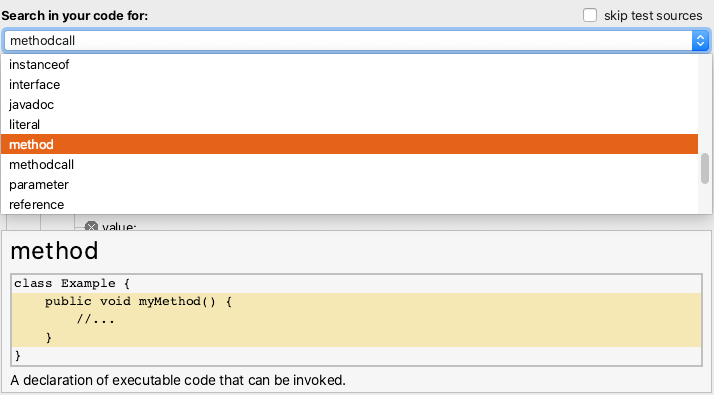
\includegraphics[width=\textwidth]{dropdownhint.png}
  \includegraphics[width=\textwidth,page=6]{04-tools/figures/figures1.pdf}
  \caption[Hints for different syntactic components in the recipe editor]{There are hints available that describe the different syntactic components that can be used in Sensei recipes. These hints are visible when hovering over the different options in the drop-down menu of the recipe editor.}
  \label{fig:dropdownhint} 
\end{figure}

In the fix menu it is possible to reuse arguments of the original code through a template language..
All users who made use of these templates, did so by copying the template from a different recipe and adjusting it to their needs.
None of the users used the suggestions available in the fix menu.

\subsection{Threats to validity}
There are many threats to the validity of conclusions drawn from the findings of these usability tests.
The number of subjects is small and the tasks they were asked to complete are artificial.
The focus of these tests is not to generalize any of the behaviours of the subjects, but rather to identify common usability problems in the interface of the recipe editor.
Several of these problems were detected.
I make no further attempts at interpreting the results from this usability test, I only report the findings as they appeared in the screen recordings.
\section{Industry trial in 2018}
\label{sec:trial2018}

One of the earliest customers of Sensei closely monitored their use of the tool during a trial period of several months in 2018.
They reported their findings to us and at the end of the trial they purchased additional licenses for the tool.

\subsection{Goal}
The \textit{goal} of the trial is for the client to observe the effects of the Sensei \gls{ide} plugin on its development process.
The \textit{purpose} is to help the client decide whether or not it is worth to purchase licenses for the Sensei \gls{ide} plugin.
The \textit{quality focus} is on the time and money saved by detecting possible vulnerabilities early.
The client aims at better estimating the return on investment of the potential purchase.
During the trial they can both collect some objective data on the amount of vulnerabilities prevented, as well as collect opinions from the application security team and the developers involved in the trial.

\subsection{Set-up}
\subsubsection{Subjects}
The client is a large bank included among the top 25 banks of the world as listed on wikipedia\footnote{\url{https://en.wikipedia.org/wiki/List\_of\_largest\_banks}}. The subjects were a group of five full-time developers selected by the client for their security knowledge. The tool was also given to an employee responsible for application security to help evaluate the trial. This employee was our main contact during the trial period.

\subsubsection{Tasks}
The subjects are part of teams developing and maintaining the web and mobile applications of the client. They were developing in either IntelliJ IDEA or Android Studio. During the trial period they continued their daily responsibilities as usual, reporting periodically to the application security expert on their impressions of the tool.

\subsubsection{Treatment}
The developers were given two sets of recipes, one for general Java applications, and one for mobile Android applications in particular.
The cookbook for general Java applications was developed internally by our developers in cooperation with the application security expert.
They advised what they wanted to achieve from the developers with the tool, and we created recipes to enforce this.
The second cookbook was also developed by us and was based on the official Android developer guidelines\footnote{\url{https://developer.android.com/}}.
All of the recipes in this set had scopes so they would only be active when the developer is working on an Android project.

\subsubsection{Information gathering}
The client did not share their code nor their Sensei events file.
Our contact was given the ability to view the summary of the Sensei events file in the form of an update to the Sensei plugin that enables them to view the statistics on each device.
Our contact at the company evaluated these and shared some of their insights as well as opinions from the subjects themselves.

\subsection{Findings}
They reported that during the trial over 200 markings were found that were legitimate markings that could lead to vulnerabilities. With the majority of these present in legacy code, they were \glspl{security defect} already in production. The two most common categories were mentioned as being tapjacking and sensitive information leakage (mostly caused by leaking stack traces).

The subjects reported the tool as very useful and not too intrusive when working on new code. They also reported improving their security knowledge, driven by the markings from the plugin.

After the trial, the client chose to extend their current licenses and purchase additional ones.

\subsection{Threats to validity}
There are many threats to the validity of conclusions drawn from the findings of this trial. We have no detailed knowledge or control over the task, the subjects, the time, or indeed over any other aspect of the trial. We are unable to account for any noise in the metrics or any conditions that limit our ability to generalize the results. For this reason we make no attempts at interpreting the results from this trial, we only report the findings as they were reported to us.
\section{Industry interview in 2021}
\label{sec:trial}

%Intro
%-------
%    Pieter - PhD in software security at SCW and University of Ghent Belgium
%    Research DevSecOps - human centered security practices
%    Some questions you might not have the answer available without looking up data
%    I will come back with an e-mail and we can see what data is possible 
%    Can I record this meeting? that way I don't have to take notes
%    Who are you? What are your roles at the company?
%    
%Team and practices
%------------------
%    How long have you been using Sensei? 
%    Size of the team? devs vs security professionals
%    How many use Sensei? Voluntarily? Changed over time?
%    How did you start using it?
%    What other tools do you use that work well or work against Sensei?
%    
%Rules creation
%--------------
%    How many Sensei rules have you created?
%    Who creates the rules?
%        - wizard? preview panels? UI view or code view?
%        - quickfixes? descriptions? scopes?
%        - do they have lots of hits?
%    Security related vs quality vs productivity?
%    Recipes to migrate libraries? Or recipes to use libraries correctly?
%    do you use any public cookbooks?
%    any rules that stand out to you, that you think show off Sensei capabilities?
%    
%Findings
%--------
%    do your rules have hits on code that you don't want to fix? or are they always accurate?
%    do the users of Sensei trust the tool and quickfixes? do they use them often?
%    Do you feel Sensei improces your code security? Do you have any evidence?
%    Do you feel Sensei boosts productivity?
%    
%    Overall impressions of Sensei?
%        - security, quality, productivity, management

In August 2021 I had the opportunity to interview the security team at a large company that has been using Sensei for over two years.
They shared their insights in how the tool is used, what they liked about it and what its biggest shortcomings are in their eyes. 
        
\subsection{Goal}
The \textit{goal} of this interview is to learn how Sensei is actually used in an industry setting.
The \textit{purpose} is to understand if our design goals align with the expectations of the users, and to observe which features are most useful and which are lacking or missing.
The \textit{quality focus} is on the frequency features are being used, and for which purpose.

\subsection{Set-up}

\subsubsection{Subjects}
The client is an international cloud computing company building and maintaining \gls{erp} software used by more than 26,000 customers.
The teams observed and interviewed are based in Europe.
They are 8 teams of developers and a team of 12 security professionals.
Most, but not all, security professionals have prior development experience, some at this same company.

\subsubsection{Task}
The subjects are part of teams developing and maintaining the \gls{erp} software of the client.
All of the Sensei users are developing using the IntelliJ IDEA.
During the use of Sensei they have continued their daily responsibilities as usual.

\subsubsection{Treatement}
Use of the Sensei plugin in these teams is voluntary.
About 90 employees in total are using the tool, of which 60 are using it more actively.
Five of the security professionals use the tool, as they are the ones involved in Java development.
The remaining users are developers.

The teams have been using Sensei for over two years.
When it was purchased, one of the security professionals gave a presentation and a demonstration of the tool to interested coworkers.
Most attendees were team leads, managers, and some security champions.
From there on, use of Sensei has not been actively promoted across the company.
However, one security professional regularly discusses the tool in the security champions group meetings, as well as the dedicated support channel on \gls{slack}.

The security team also uses Fortify, Checkmarx, SonarQube, Semgrep, and FindBugs.
They have sufficient context to compare Sensei to other security tools.
The listed tools, together with other comparable tools, are discussed in more detail in Chapter~\ref{ch:related}.

\subsubsection{Information gathering}
The team of security professionals is our contact at the company.
Two members of the team agreed to a meeting in which I interviewed them on their use and their impressions of Sensei as well as other security tools they are familiar with.
This interview was recorded and the recording reviewed before writing this report.

One of the interviewees has been with the company the entire time that Sensei was purchased, this person has prior development experience.
The other interviewee joined the company after the purchase of Sensei, this person does not have prior development experience, but has been a security professional for a longer time.

\subsection{Findings}

\subsubsection{Adoption}
The security professionals found that adoption of the tool is not easy.
It is hard to get a chance to show value to the developers, and they are hesitant to install new tools in their \gls{ide}.
It is easier to convince the security champions who are more interested, and actively looking for tools that can help them produce secure code faster.
So far the security professionals have preferred the hands-off approach and allowed the tool to organically spread, instead of making it mandatory.
The security professionals, many who have development backgrounds, are convinced that the tool can be an asset to developers outside of the context of security as well.

\subsubsection{Recipes}
The security professionals have created around 50 recipes.
They are stored on a remote server and distributed to the developers as a read-only cookbook.
The recipes in this cookbook are not all security related, but around 70\% of them are.
The other recipes are related to quality and code conventions.
Many of the security team have a development background, they have added these recipes in an attempt to show their value to the developers.
No public cookbooks are used, but the recipes in the public cookbooks served as inspiration for their own custom recipes.

The company has a lot of very clear coding standards that are published and used outside of their company as well.
These coding standards are used as a basis for recipes and their quick-fixes.
No real consultation with developers is needed, as it is generally agreed by developers and security experts that these coding standards are to be used.
However, to create the quick-fixes, the security professionals frequently consult internally with more experienced team members.
Since some of them are former developers at the same company, they have an intimate knowledge of the code base.

The company uses many wrapper libraries.
However, these are often not specifically written for security purposes only.
Several Sensei recipes exist to migrate to wrapper libraries or to different versions of \glspl{api}.

The security team is currently unaware of the amount of recipes that are being created by developers themselves.
They are also unaware if developers are frequently remediating markings from the distributed cookbook.
In fact, in their eyes, visibility into metrics like this is one of the biggest shortcomings of the tool.

\subsubsection{Recipe editor}
The security professionals create both recipes from scratch and from context and think both use cases are important and necessary.
They most frequently use the \gls{ui} view to edit recipes, but to refactor recipes and make bulk changes, they sometimes use a text editor as well.

They think the preview panels and the recipe editor are by far the most useful features of the entire plugin.
These features make customization of the recipes far more easy compared to the other tools they are using in the \gls{sdlc}.

Descriptions are often used, but the full coding guidelines are not usually customized to the specific recipe.
The coding guideline provided is instead a generally applicable description that provides links to documentation about the secure coding standards that are used at the company.

The security professionals use recipe scopes very often.
The scopes are used to limit recipes to certain packages and modules.
This is only done as a consideration for developer usability, to avoid false positives in the large code base.

Finally, they try to provide quick-fixes as often as possible, but admit it is not always possible.
Sometimes the quick-fix provided requires the developer to make additional changes.

\subsubsection{Paved path methodology}
The security team is not using a paved path methodology.
However, their practices are in line with many of the goals of this methodology.

The security professionals try to be \textit{enablers}, and not only tell developers what they do wrong, but also provide guidance as much as possible.
They provide a service to developers and are very aware of developer usability.
The team prefers to neglect some parts of the security of the software over generating too many false positives, which could result in \glspl{efp}.

They belief Sensei supports this enablement approach through its quick-fixes.
Since a complete Sensei recipe includes a quick-fix, the security team is forced to offer remediation guidance.
This remediation guidance in turn enables the developers to resolve security markings by themselves.

For the security professionals without former development experience, this requirement of a quick-fix forces them to be closer to the development workflows.
Sometimes, creating a quick-fix pushes the limits of their knowledge of programming.
In that case, they do not consult the development team, as suggested by the paved path methodology, but instead consult with former developers in the security team itself.

\subsubsection{Disadvantages}
As mentioned before, visibility into the developer's practices with the tool is one of the biggest shortcomings of Sensei in the eyes of the security team.
So far features that report back information from the \gls{ide} have been avoided as we expected customers would be hesitant of such features.
Many of the metrics that the security team requests are available in the \glspl{ide} of the developers, in the Sensei events databases.
Clearly, gathering those databases is not a convenient way to collect that information.
On top of that, currently we provide no convenient way visualize the results in a management dashboard, which other tools commonly provide.

Alternatively, some metrics can be collected through server side scans.
It is possible to run IntelliJ IDEA inspections from the command line, including the Sensei recipes. 
The resulting scans are not as efficient as those by standalone tools, such as static analysis tools discussed in Chapter~\ref{ch:related}.
In particular, the memory usage is exceedingly big for large enough code bases because the entire \gls{ide} is in fact running in a background process.
It is also more difficulty to automate running IntelliJ IDEA inspections in the \gls{cicd} pipeline compared to tools who provide better integrations for this purpose.
The convenience of running scans in other stages of the \gls{sdlc} seems to be the main reason the security team uses some of the other tools.

%
%== Other tools
%FindBugs
%--------
%Creating rules with is harder, not as intuitive
%Can be more easily integrated in CI
%Simple general rules that are more widely applicable, and make more sense in CI
%Not usable in shift left
%No remediation
%They want rules in CI and in the IDE to show the same things
%
%SemGrep
%-------
%used by security professionals in the code reviews, in between developing and building
%without dev, reactive feedback, more automated
%links to documentation as feedback, no code fixes
%rules are pretty easy to customize but it is more difficult without the preview panels, it is better than findbugs
%semgrep is multi language
%compile agnostic, fully realised on text (no AST), so no compilable classes are required, code snippets are enough
%
\subsection{Threats to validity}
There are many threats to the validity of conclusions drawn from the findings of this trial. We have no detailed knowledge or control over the task, the subjects, the time, or indeed over any other aspect of the trial. We are unable to account for any noise in the metrics or any conditions that limit our ability to generalize the results. For this reason we make no attempts at interpreting the results from this trial, we only report the findings as they were reported to us.
%\section{Marketplace users}
\label{sec:marketplace}

The Sensei \gls{ide} plugin has been release for free on the JetBrains marketplace on September 10, 2020.
During this time many developers have installed and uninstalled the plugin.
We have collected metrics to give us insights into what makes a user keep using Sensei, or what causes them to uninstall it.


%Churn rate:
%(confidential? Can I share this data? Probably not)
%the insights might be useful, but the exact numbers can not be shared
%
%Opened cookbook manager:
%never, 350, 134
%once, 64, 61
%twice, 24, 26
%3 or more times, 34, 67
%
%Added cookbooks in the cookbook manager
%0 cookbooks, 109, 141
%1 cookbooks, 13, 13
%
%Churn by days till the cookbook manager is opened
%never opened, 490, 154
%day 0, 123, 103
%day 1, 7, 9
%day 2+, 24, 87
%
%churn by opening recipe editor
%0 times, 456, 258
%1+, 15, 21
%
%churn by days till open recipe editor
%never opened, 624, 318
%0-1 day, 16, 11
%1+ days, 5, 26
%
%Most people install early on:
%Most people who make it past a week, stick around 


\chapter{Discussion and Perspectives}
\label{ch:tool-eval}

In the previous chapter I described the goal and the set-up of each experiment, and reported their findings.
These findings allow us to evaluate different features of the Sensei plugin, as well as its use in the paved path methodology.
In this chapter I summarise the findings, explain the lessons we learned and how they can affect the development of Sensei in the future.

\summarybox{
Our findings and those of other research, shows that customization of recipes can have a significant impact on the \gls{efp} rate, and hence the usability for the developer.
Using customized recipes results in a positive impact on the codebase since security issues are addressed truly as early as possible in the \gls{sdlc}.
If designed properly, applying the recipes regardless of context has minimal impact on performance, and helps improve code quality in many cases.

Security professionals report that creating these customized recipes with the recipe editor is easier than customizing rules of comparable tools.
Despite this, usability tests revealed that some features of the recipe editor can still be improved.
}


\section{Discussion}
\label{sec:eval-sensei}
\subsection{Installation and first use}
Because Sensei is distributed as an \gls{ide} plugin, it can be easily installed from the \gls{ide} itself, using features that many developers are familiar with.
None of the developers in any of the experiments needed more than several minutes to install the plugin.

After installation, the startup time of the \gls{ide} is not measurably affected by the tool.
Sensei only performs a license check, of which the duration is shorter than the measured variation in \gls{ide} start-up time.

In the early industry trial and the controlled experiment, customized Sensei rules were provided by us as a service.
In the usability tests and the most recent industry trial, the subjects were provided with public cookbooks that could be used as a starting point, but they were encouraged to create their own recipes.

In both groups we have observed developers who unknowingly addressed Sensei markings, thinking they were regular \gls{ide} markings.
This is strong evidence that the tool is intuitive and feels like a natural extension of the \gls{ide}.

\subsection{Recipes}
Sensei is a developer tool first, and this is evident from the recipes that are used in industry settings.
A significant portion of the recipes are related to the quality of the code rather than its security.
%Many Sensei recipes are also written to boost the productivity of the developer.
%One example is a set of recipes that was created to migrate from JUnit version 4 to version 5~\footnote{\url{https://junit.org/}}.

We have noticed, in practice, that security and quality are often closely related.
High quality code is easier to understand and maintain, and hence also to secure.
But often, writing high quality code can also lead to secure code in a more direct way.

Take the example of a \gls{sql} query.
Writing a data retrieval method of high quality means that the query is easy to understand, but also that the data is retrieved at high speed.
When the query is parameterized, the database can pre-compile a query plan, which speeds up the execution of the query.
Of course, using parameterized queries at the same time ensures that the query is safe from \gls{sql} injection.
Even if the current query did not use any (unsanitized) user input, using a parameterized query will protect it from future use.
It will also set a good example for future developers writing similar methods.
Developers will often copy existing code and make some changes to fit their needs.
After all, developers try to be as efficient as they can in delivering code.
If no parameterized queries are used, a subtle change can mean the difference between secure code or a vulnerability, as shown in Listings~\ref{lst:safe}~and~\ref{lst:unsafe}.

\begin{lstlisting}[float,language={Java},caption={This method concatenates an integer value to the query. An integer variable can not alter the query, and hence this method can not lead to SQL injection.},
float,label={lst:safe},abovecaptionskip=-0.0pt]
public ResultSet getUserById(int id){
    String query = "SELECT * FROM user WHERE id = " + id;
    PreparedStatement stmt = this.conn.prepareStatement(query);
    ResultSet rs = stmt.executeQuery();
    return rs;
}
\end{lstlisting}

\begin{lstlisting}[language={Java},caption={This method concatenates a String variable to the query. As a result it is vulnerable to SQL injection.}, float,label={lst:unsafe},abovecaptionskip=-0.0pt]
public ResultSet getUserById(String id){
    String query = "SELECT * FROM user WHERE id = " + id;
    PreparedStatement stmt = this.conn.prepareStatement(query);
    ResultSet rs = stmt.executeQuery();
    return rs;
}
\end{lstlisting}

In industry, recipes were created, both to help developers use libraries correctly, as well as to migrate to new libraries.
Security professionals reported that many wrapper libraries are used in their codebase to make the life of developers easier.
These wrapper libraries were rarely developed solely for security reasons, but often did include security automation.
It is clear that for such wrapper libraries, it is crucial that the recipes can easily be customized.

\subsection{Recipe editor}
When testing \gls{yaml} syntax and creating recipes from context, we observed a significant speed-up in writing recipes.
Even for users that were experienced with the old rule models, the preview panels in the new recipe editor and the context-aware suggestions greatly improve the recipe-writing process.

Security professionals report that Sensei is the easiest tool they have used when it comes to customizing recipes.
The majority of comparable tools allow writing custom rules or analyses in some way or another.
\todo[inline]{revisit after related work is finished}
Writing rules for these tools is done through complex, but well documented \glspl{api} (SpotBugs, Tricorder, Checkmarx) or more user-friendly custom formats such as \gls{xml} (Fortify, SecureAssist).
Of these, Checkmarx is the only one tool that provides a Query editor and manager, albeit not built into their static analysis tool.
For all other tools, the rule writers can use an \gls{ide} or text editor of their choice.
None of the tools allow creating rules on-the-fly in the code.
Sensei does allow this, which greatly improves the speed and usability of writing rules.
Related tools will be described in more detail in Chapter~\ref{ch:related}.

\subsubsection{Recipe features}
Because recipes can be created on-the-fly in the code, context-aware suggestions can be made, and testing of the recipes is more efficient since their markings can be observed live as the recipe is being created.
This live preview in the recipe editor is mentioned by the security professionals as Sensei's most useful feature.
Despite this, some of the features of the recipes and the recipe editor are not used as often or as effective as they could be.

When security professionals and developers create new recipes, they rarely use the code view.
In fact, we have noticed that the code view can be overwhelming for some users who want to avoid learning a new language.
To create recipes from scratch, and to adapt existing recipes, almost exclusively the \gls{ui} view is used.
The code view is only used by recipe-writers when copy-pasting recipes from the documentation or from recipes used as an example.
The \gls{gui} can be updated to better reflect this behaviour.
The \gls{ui} view should be the main focus when opening the recipe editor, and the code view can be made smaller as its main focus is to copy-paste examples.
The resulting \gls{gui} will have a similar user experience as the \gls{ui} provided by \gls{slack} to customize (and share) color themes, as shown in Figure~\ref{fig:slacktheme}.

\begin{figure}
  \centering
  %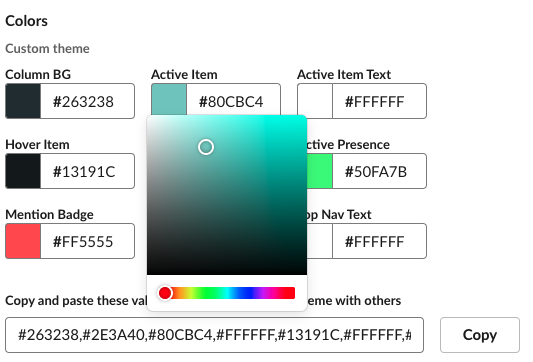
\includegraphics[width=0.75\textwidth]{slacktheme.png}
  \includegraphics[width=0.75\textwidth,page=16]{04-tools/figures/figures2.pdf}
  
  \caption[Slack theme editor]{The theme editor in slack provides an intuitive \gls{ui} interface on top to edit the theme, but also adds an code view and a copy button to allow fast and easy copy-pasting of existing themes.}
  \label{fig:slacktheme} 
\end{figure}

Security professionals report using the context-wizard to automatically generate recipes from context.
However, in usability tests, none of the tested users have used this features.
This indicates that the feature might not be clearly understood.
Instead of “create recipe for similar methodcalls”, it might be more effective to make the option in the menu adapt to the context, for example “create recipe for Runtime.exec methodcalls”.

Quick-fixes are added to nearly every recipe.
However, in some situations no fully functional quick-fix can be created and the developer is still required to make changes to the code after applying the quick-fix.
The template language that allows reusing parts of the original code is often required to create a working quick-fix.
However, the suggestion box in the quick-fix menu is not clearly visible to the users, and as a result these suggestions are rarely used.
The recipe-writer can still find them in the documentation or by copy pasting from other rules, but using this menu should be more convenient.
Currently, the variables are hidden by default and the ``Show variables" button is not prominent enough, as shown in Figure~\ref{fig:showvariables}.

\begin{figure}
  \centering
  %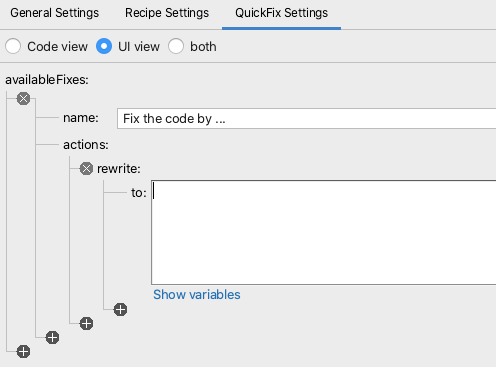
\includegraphics[width=0.75\textwidth]{showvariables.png}
  \includegraphics[width=0.75\textwidth,page=15]{04-tools/figures/figures2.pdf}
  \caption[Show variables button in the fix menu]{The suggestions in the quick-fix menu are hidden by default. Users do not make use of the ``Show variables" button that reveals them, as it does not attract their attention.}
  \label{fig:showvariables} 
\end{figure}

Scopes are used frequently in industry, almost exclusively to avoid creating \glspl{efp} and increase developer usability.
Most of the comparable tools operate in later stages of the \gls{sdlc}.
They perform scans during code review or testing phases.
Usability issues for these tools are less critical as they do not create markings that can disturb a developer during development.
Instead it is often a security expert who will analyze and prioritize the results of security scans by placing them into the bug tracking system.
Common features for those tools are integrations with common bug tracking systems to allow them to publish bugs automatically.

We observed that many tools provide functionality to disable certain rule reports through configuring security policies.
This is a necessary feature to remove or hide classic false positives.
However, this disabling of reports is designed to help security experts keep a good overview of the application state and to help prioritize more severe issues.
With the exception of the Fortify Security Assistant that disables rules to speed up the scans, disabling rules themselves is rarely supported with he goal to improve the usability of the developers.

\subsection{Feedback and remediation}
Sensei is distributed as an \gls{ide} plugin.
This allows it to reuse and extend existing \gls{ide} functionality, and naturally feel part of the existing tool kit of developers.
When interviewed, subjects of the usability tests reported that the markings and quick-fixes felt similar to those provided by the \gls{ide} itself.
They all indicated that they would use them frequently.

When analyzing newly written code, the longest time we have measured that is needed for the analyses to finish is 29 ms.
This is far below the threshold of 125 ms to be considered real time.
A developer is hence not hindered during development unless they are violating a coding guideline and need to use remediation.

When code is marked, the developer needs to spend some extra time understanding the issue and fixing it.
During the empirical experiment of Section~\ref{sec:experiment}, the mean observed remediation time of a guideline violation is 19 seconds.
On average, the use of Sensei increased the total development time with 11\%.
This is a relatively low increase considering the programming assignment was to complete security-critical features and hence the subjects were frequently confronted with feedback from the tool.
It is also important to note that for all of the subjects, the experiment was the first time they were making use of the tool.

During the experiment, 98.4\% of code markings shown by Sensei (n = 247) were resolved by the developers.
Out of the resolved code markings, 73.3\% were fixed using the quick-fixes.
All of the users (n = 15) used at least one quick-fix, with an average of 12.71 (s = 4.73) quick-fixes used.
The remaining code markings have been removed manually, either by fixing the violation or by removing the violating code entirely.
This is a high level of engagement, compared to the lower than 20\% ``Apply fix" rate reported by the code review tool Tricorder~\cite{sadowski2015tricorder}.
On average the subjects resolved the issue within 19.10 s (s = 25.22 s) of writing the violating \gls{api} call.
Developers appear to be spending comparatively little time understanding the issues and applying fixes.
By comparison, for Tricorder and SpotBugs the time between writing the violating code and fixing is usually several days~\cite{sadowski2015tricorder,ayewah2007using}.

In the experiment with Sensei, only 1.6\% of code markings were ignored, which is a low \gls{efp} rate.
After carefully improving their analyzers, Tricorder reached an \gls{efp} rate of around 5\%.
Despite its great attention to developer usability, during an experiment with ASIDE, only 63 of 101 markings were addressed~\cite{xie2011aside}.
When using SpotBugs, research reported that 58\% of the reported issues were never reviewed and out of the reviewed bugs, only 55\% were eventually fixed~\cite{ayewah2007using}.
We observe a big gap in \gls{efp} rates with Sensei and Tricorder having a rate of 5\% or lower on one hand, and Aside and SpotBugs having 38\% and 77\% on the other hand.
The reason for this might be the customization of rules.
Tricorder allows creating new analyzers and their quality is closely monitored.
For Sensei, developers are given carefully tailored rules, often written by the engineers themselves, and relevant to their project.
These efforts are clearly greatly improving the usability of the tool and hence the trust of the developers.

\subsubsection{Impact on security}
The usability measurements presented so far suggest that when Sensei is used, the secure coding guidelines are applied most of the time.
During the first undustry trial of the plugin, described in Section~\ref{sec:trial2018}, the client has tracked closely whether or not the enforced guidelines actually prevented the introduction of vulnerabilities early on.
The trial was done with five developers for the duration of three months.
They reported a total of over 200 confirmed bugs being prevented.
The most common issues involved sensitive information leakage and tapjacking vulnerabilities in their mobile application.

A limitation of the tool's local analyses is that they do not allow us to detect whether or not a certain input has already been sanitized before flowing into the routine being analyzed.
This is in line with our approach and goal of enforcing coding guidelines that defend every routine for future use, i.e., such that it is still secure whenever it might be reused with unsanitized data.
So if the local analyses identify a lack of local sanitization, the developer will be expected to let the routine sanitize that input again.
At first sight, this might result in the same data being sanitized multiple times within an application, which will negatively impact performance. 

In practice, however, this proves to be largely a non-issue.
In practice, \glspl{api} are not designed in a vacuum.
Instead they are developed with potential application architectures in mind.
Furthermore, when concrete applications are first designed, security and application architects also take into account best practices for secure architectures (that is, if they care for security-by-design).
Similarly, the coding guidelines can be co-designed with certain application architectures in mind.
Doing so provides an easy mitigation of the potential issue of redundant, multiple sanitizations.

For example, consider the case of \gls{xss} attacks.
It is a common misconception that in order to prevent stored \gls{xss} attacks, user input should be encoded before it is stored in the database.
A better recommendation is to encode the database output when it is used, as the stored data may be used in different contexts, requiring different encoding methods.
For example, a string value may be displayed on the \gls{html} page and also used in a JavaScript script on that same page, resulting in two different, but simultaneous escape requirements.
We learn that data should always be sanitized before it is stored in the database and encoded before it is displayed in the web or mobile application.
Since these are usually the ends of the data flow, no data needs to be sanitized or encoded twice.
If the rules are co-designed with the secure application architecture, it becomes trivial to enforce the sanitization and encoding routines at the correct locations in code. 
The above does not imply that Sensei is the one and only tool that solves all potential software development security issues.
To detect issues as early as possible, i.e., in real-time as the developer is writing code, analyses have to be light-weight.
This implies that all possible execution paths in the entire program cannot be exhaustively considered, and some types of vulnerabilities, including design flaws, can go undetected.
This is a common trade-off, therefore tools that are used early in the \gls{sdlc} such as Sensei should be complemented with more complete scanning solutions deployed later in the \gls{sdlc}.
\todo[inline]{revisit after related work}
Security professionals understand this.
In the second industry trial Sensei is complimented by five additional security tools: Fortify, Checkmarx, SonarQube, Semgrep, and FindBugs.

An example of this strategy also exists with multiple products of the same company. 
The Fortify Security Assistant \gls{ide} plugin is used earlier in the \gls{sdlc} than other Fortify tools, but only uses a subset of the available rules to improve developer usability.
It helps detect a set of vulnerabilities earlier, and hence saves money and time fixing those issues, but it does not provide the full protection that, e.g., Fortify on Demand does.
In the related work section, we will discuss where we consider Sensei to improve over Fortify Security Assistant as an early \gls{sdlc} tool.

\subsection{Project and team management}
\subsubsection{Compliance}
Coding guidelines can provide a good measure for security in a software product.
Where vulnerability scanning can only provide an indication of the vulnerability density, they do not provide the full picture.
In the case, for example, where a large number of \gls{sql} injections is found, this could indicate poor database security.
But it can also mean that there simply are a lot of database queries, with a large portion of them done securely.
For coding guidelines a relative measure can be designed, by comparing the number of guideline violations to the number of times the code complies to guidelines. Since complying to strong coding guidelines leads to secure code~\cite{banerjee2009software,tabassum2017comparing}, we get a better indication of the security in the software product.

While the plugin is useful as a tool to aid the developer, the option to measure guideline deployment also hints at its potential as a management tool.
Like we did for the empirical experiment, management can track the changes developers makes to projects and log the guideline violations that they introduce and fix, with or without aid of the quick-fixes.
Currently, this data is collected in the events databases on the machine of each developer.
In the future, these metrics will be collected and visualised on the \gls{scw} platform.
This makes the return on investment clear to companies using the tool.
Furthermore, this can be used to track the performance of individual developers, and then to give more targeted and individually tailored training.
This data can for example feed into the \gls{its} to improve its recommendations, as described in Section~\ref{sec:its-integration}.

\subsubsection{Integration in other stages of the \gls{sdlc}}
While individual performance can hence be measured and improved, with developers working in different branches, and hence different states of the project, it is hard to get a good overview that way.
To resolve this, we also give managers the possibility to use the plugin technology as a headless scan that can be performed from the command line.
However, in practice, we have noticed that the performance of this headless scan is lacking.
Especially for large codebases, memory usage becomes exceedingly large.
Security professionals also indicated that better integration with \gls{cicd} tools is needed.
This lack of automation in different stages of the \gls{sdlc} is critical for the security team.
The security professionals in the second industry trial have spent time and effort to recreate Sensei recipes in different tools in the \gls{sdlc} to compensate for Sensei's lack of \gls{cicd} integration.
While the tool is a developer tool first, it is also a security tool, and it is usually purchased by the security team.
Which is why it is important to show value for both user groups.

\subsubsection{Roll-out}
From experience, we learned that the plugin is ideally rolled out when new recipes do not mark any existing code.
This is when a project kicks off and zero lines of code have been written. 
Alternatively it can be rolled out when a new \gls{api} or library is introduced in the project and recipes will be written for this library or \gls{api}.
Few projects are developed from scratch, however, so the reality is that the plugin needs to work in an already developed product.
In that case, rolling the plugin out with all recipes switched on can be overwhelming to developers, as they are presented with a huge number of violations.
In addition, developers are often hesitant to fix issues they did not introduce in the code themselves, and they might not even have permission to change code that is not theirs.
This results in a large number of \glspl{efp}, which we want to avoid.

When developers create their own recipes from scratch, they are working on a certain branch of the project.
They usually create targeted recipes to fix or enforce small things in the project files they are working on.
When they create the recipe, they inspect the violations and fix the markings.
The recipe and fixed code are pushed to the codebase simultaneously.
This typically leads to few \glspl{efp}.
However, often the application security team of the company imposes recipes as well.
At one point, the security expert at a client of ours created a large number of recipes and imposed them onto the developers without fixing any of the resulting violations.
It did not come as a surprise that this resulted in a great number of \glspl{efp} and out of the 20 developers that had the tool installed, all of them had disabled its markings.
To avoid such failures, we recommend two approaches to keep the \gls{efp} rate low for imposed cookbooks.

Firstly, in the ideal scenario the security team creates a number of recipes and looks at their violations in the code to inspect their severity.
When recipes result in few violations, the team can safely roll out the recipes without resulting in too many \glspl{efp}.

The roll-out is more challenging when a recipe results in a large number of violations that are not trivially resolved.
In that case the security team should create a developer task force.
Their task is to create \glspl{api} to resolve the recipe hits.
They then turn the original recipe into a library adoption recipe and fix all marked code with this recipe.
In the process of doing so, many corner cases can be encountered that help to fine-tune both the \gls{api} and the recipe.
The new \gls{api}, the recipe, and all code fixes can be pushed to the codebase simultaneously. 

The ideal scenario might not apply in practice, however.
It is possible that the codebase is simply too large to start fixing all code markings.
We have had clients where a strong recipe resulted in over 3000 violations.
It can also be the case that when the security team creates a task force, this developer time is paid by the security budget, not the development budget.
In such cases it is not beneficial to spend developer time to fix the existing issues in the code before rolling out the recipe. 

We then instead recommend the second approach, in which the recipes are rolled out company-wide without fixing the code markings.
In order to keep the \gls{efp} rate sufficiently low, the violations are only shown partly.
For this purpose the option is added to the recipe editor, to only mark a recipe on newly developed code.
This way only new violations are shown (and resolved) without resulting in an overly large \gls{efp} rate.
\section{Perspectives}
\label{sec:sensei-perspectives}
%\todo[inline]{intro}

\subsection{Improved recipe creation}
\label{sec:improvedrulecreation}
Security professionals report that Sensei is the easiest tool they have used when it comes to creating new recipes.
They attribute this mostly to the preview panels in the recipe editor, rather than the specific \gls{yaml} syntax.
Developers, on the other hand, are not used to creating rules for any tools, so they usually have nothing to compare it to.
This is evident from the usability tests, where developers were more hesitant and more easily overwhelmed by the recipe editor compared to the security professionals.
To reduce this hesitation, in the previous section, a design was proposed that would make the \gls{ui} view the main focus in the recipe editor.
In this design the code view would only be used for copy-pasting recipes.
However, this still requires developers to create recipes for an analysis tool, a task they are not familiar with.

Instead, it might be possible to let developers create recipes simply by writing code.
Currently, Sensei is able to apply a code transformation based on instructions from a recipe.
In the future, it might be possible to do the opposite, and generate a Sensei recipe from a code transformation.
If this technology exists, the recipe editor can simply show two code panels side by side.
The left panel can be a static view of the current state of the code, while the right panel allows the developer to make (small) changes to the code.
A Sensei recipe can then be created from the code changes that can optionally be adjusted in the next step.

This technology would also enable automatic recipe creation methods, such as generating a recipe from a code patch in the code repository.
It might even be possible to dynamically suggest recipes while observing the developer during their normal workflow.
Previous research has been performed to identify \gls{api} rules for cryptography from code changes~\cite{paletov2018inferring}.
Efforts have also been made to automatically generate patches from code repositories and their histories, using different algorithms~\cite{weimer2009automatically}, including those learned from human-written patches~\cite{kim2013automatic} or correct code~\cite{long2016automatic}.
While this research tries to automatically patch bugs, the approaches can also be used to create recipes to apply the discovered patches more broadly and to do so during the writing of code rather than afterwards.
With some user interaction, such a tool might also be able to generate recipes (without fixes) from the output of traditional security tools.

This technology is part of ongoing research funded by a \gls{vlaio} \gls{oeno} project as of 2019.

\subsection{Adapting feedback to the skill level}
An important concept during the design and evaluation of the Sensei \gls{ide} plugin, is the \gls{efp} rate.
When many markings exist in the code that the developer does not intend to fix, i.e., when there is a high \gls{efp} rate, this might cause developers to be overwhelmed and ignore feedback from Sensei altogether.
To explain this concept, the example of \gls{os} command injection was used.
A simple and easy to understand recipe to avoid \gls{os} command injection, is to simply avoid all uses of \gls{os} commands.
A more experienced developer, however, will understand how \gls{os} commands can be used securely, for example to launch a different software application through a hard-coded command.
This recipe will lead to an \gls{efp} for an experienced developer, but might be more easily understood by a developer with no security skills than a more advanced recipe.

In other cases, recipes are created that detect (presumably) deliberate insecure configurations.
Take the example of cookies, where it is generally recommended to configure them as HttpOnly.
This prevents the cookies from being used in client-side scripts, and hence avoids some of the most common \gls{xss} attacks.
However, in some legitimate cases the developer might need to use a cookie in a client-side script, and to configure the cookie as such.
Of course, they have to take the security implication of this configuration into consideration.
For example, they will have to ensure that this is not used for security-sensitive cookies, such as session cookies.
A recipe that detects insecure configurations like this, will lead to \glspl{efp} for developers who need the features that are blocked by these configurations.

Both the example of the \gls{os} command and cookie configuration, lead to \glspl{efp} for security experts, but are still important recipes to enforce for a novice developer.
Fortunately, through integration with the \gls{scw} portal, a user ability estimate is available, such that the feedback for recipes like this can be adapted to the skill level of the developer.
For developers with a low ability level, this recipe can be shown as an error, while the more experienced developer can be shown a warning or information level marking.
The descriptions can also be adapted for each skill level.
The less experienced developer can be shown the simple and easy to understand guideline, to use the most secure configuration.
To a more skill full developer it will be less overwhelming to explain the security implications of the configuration, and how to mitigate them in other parts of the code.
Adapting \glspl{ui} is most often based on the experience of the user with the interface itself rather than their knowledge in a specific field~\cite{johnson2015bespoke, cockburn2014supporting}.
This research indicates that optimizing \gls{ui} design based on novice learning rather than long-term efficiency by experienced users can be counterproductive.
It remains future work to assess whether or not a more optimised \gls{ui} will be required for advanced Sensei users.

\part{Related work}
\label{p:related}
\epigraph{Read them have you? Page-turners they were not.}{\textit{Yoda}}

\chapter{Security in software development}
\label{ch:related}

Software security is a relatively new field~\cite{mcgraw2004software}, but many tools and practices have already been developed that have caused great advancements.
Many guides exist to help you decide which tools are appropriate for your project.
In this chapter, I want to extend these guides so that you are better equipped to estimate the strengths of a tool for use in the paved path methodology.
I describe commonalities between tools in different phases of the \gls{sdlc} and how they can be deployed effectively.

For future reference, Appendix~\ref{app:battlecards} contains a number of battlecards with my thoughts on a few more tools.

\summarybox{
Security begins even before code is written.
Laws, legislations, and consumer demands all impact how much attention is given to security.
Besides lightweight linter tools, developers can also find help to produce secure code from patterns, libraries, and frameworks.
In the build phase, the use of new methodologies has driven the automation of building executables and installing dependencies, which has made it easier to test for use of vulnerable components.

Most security practices, however, take place in the test phase.
Many code review practices and tools exist, most of which allow customization of the rules through one of three methods: an \gls{api}, a custom query language, or a formatting language such as \gls{xml} or \gls{yaml}.
Finally, in the release phase, advancements in infrastructure as code have made it easier to securely deploy applications and manage infrastructure.
}

\section{Governance}
\label{sec:related-plan}

\subsection{Training}
Training has always played a critical role in software development, because standard computer science and engineering education often neglects software security.

Companies should first offer security awareness training to all employees involved in the software development life cycle.
Security awareness training does not necessarily need to be tailored to a specific audience.
Developers, \gls{qa} engineers, project managers, and operators can all partake in the same training.
A generic introductory course like this however is insufficient, the next step is to provide role-specific individual training.
As explained in this work, developers should be taught secure coding, and not follow training intended for security professionals or penetration testers.

In the ideal scenario, a company should also verify or provide training for vendors and contractors.
They should require annual refreshers for all employees and can host software security events to nurture a good security culture.

\subsection{Compliance and policy}
Software security is not only a problem of enablement.
Good enough training, tools, and processes exist today that can embed security in software development from the start.
Yet, we still see frequent reports in the media of bad software practices and vulnerabilities that easily could have been prevented.
The reality is that businesses often prioritize getting to market and getting new features out, over their obligations in terms of security.

\subsubsection{Privacy and trust}
The resulting security problems, however, do not only hurt the business, they also hurt the consumer.
When businesses are hacked, it is often private data of consumers that is leaked.
Recently, consumers have claimed control and rights over their personal data.
Legal frameworks have been built around data privacy, forcing businesses to consider data protection more seriously.

Most famously the \gls{gdpr}, a law on data protection and privacy, is enforced in the \gls{eu} since May 25, 2018~\cite{gdpr}.
It contains regulations that strengthen the individual's fundamental rights in the digital age and clarify rules for businesses storing or processing personal data of individuals in the \gls{eu}.
This law forces businesses to consider security more seriously, as it is estimated that at least 25\% of software vulnerabilities have \gls{gdpr} implications~\cite{gdprhackerone}.
Non-compliance with the general data processing principles in this law can result in significant fines, for example in June 2021, Amazon was fined €746 million\footnote{\url{https://www.enforcementtracker.com/ETid-778}}.
Two years after the implementation of the \gls{gdpr}, the \gls{ec} found that individuals' knowledge about data privacy has increased, and as a result privacy has become a competitive quality for companies which consumers are taking into account in their decision-making~\cite{gdprfra}.

Security is no longer just a necessary cost during development, but businesses are able to see a more direct \gls{roi} for high quality software security.
Businesses put more effort into the appearance of having trustworthy data protections in place, a process called trust management~\cite{cassandra2021analysis, ashraf2020role}.
In this discipline, consumer trust is the end-goal and good security practices are a mean to this goal.
To convince consumers and buyers of software to trust a product, businesses can acquire a seal of approval from a third party to prove they adhere to certain standards.
One such widely known certification is the \gls{iso}/\gls{iec} 27000-series, or ISO27K for short.
The series provides best practice recommendations on information security management, covering privacy, confidentiality, and other cybersecurity issues~\cite{iso27k}.
Other regimens that companies often aim to comply with are \gls{pci} and \gls{hipaa}.
To add transparency, businesses can also provide a \gls{sbom}, that lists all components used in their software~\cite{sbomntia}.
Such an \gls{sbom} is most easily produced using build tools as explained in Section~\ref{sec:related-build}.

In the \gls{us} Biden \gls{eo} on Improving the Nation's Cybersecurity issued May 12, 2021 the \gls{nist} was ordered to publish guidelines regarding practices that enhance the security of the software supply chain.
Besides providing the purchaser with such an \gls{sbom}, there are numerous other standards and procedures listed regarding trust, multi-factor authentication, encryption, and use of automated security tools.
In this \gls{eo}, \gls{nist} is directed to solicit input from the private sector and academia to develop standards, tools, and best practices.
Among the more than 150 position papers, dr. Matias Madou, dr. Brian Chess, and I have also submitted two.
One position paper advises the creation of a certification framework for education in secure development practices.
The second promotes the use of the paved path methodology.
Time will tell if this \gls{eo} makes a similarly big impact as the \gls{gdpr}.

Besides the \gls{gdpr} and the \gls{us} \gls{eo}, there are of course similar laws in other parts of the world such as the Data Protection Act in the United Kingdom, the Privacy Act in Canada, and the Personal Data Protection Bill in India.

\subsubsection{Law enforcement access}
Unfortunately, no discussion on laws and data privacy would be complete without mentioning laws on the collection and storage of electronic communication and their access by authorities.
Many of these laws contain requirements that force operators of end-to-end encrypted systems to undermine this encryption, so that law enforcement can be provided access to user communications.
One such example is the draft considered by the Belgian government at the end of September 2021\footnote{\url{https://ibpt.be/index.php/operateurs/publication/annexe-1-dispositif}}.
Under this law, operators would have to be able to ``turn off" encryption for specific users, essentially creating so-called backdoor access.
The consensus among cybersecruity experts is that there is no way to provide third party access like this to end-to-end encrypted communications, without also creating encryption backdoors and vulnerabilities that can be exploited by malicious third parties~\cite{bliss1996effective}.
Creating a backdoor like this, undermines the whole security of the system and puts its users at risk~\cite{encryptionmyths}.

In other countries where similar legislations have passed, such as Australia, research has shown that this has discouraged companies from offering new end-to-end encrypted products~\cite{barker2021economic}.
It is safe to say that policy makers and governments can have a big influence on the security of software products, for better or for worse.
\section{Develop}

Developer toolkits evolve over time, and many new technologies and frameworks exist to help developers produce code more efficiently, and more securely.
As explained in Section~\ref{sec:traditionalsecurity}, security tools are handed to the developer as well because a shift left movement is ongoing to try and identify possible security problems as early as possible in the \gls{sdlc}.
These tools, however, still use a reactive testing-based approach and can usually only identify security problems once sufficient code has been developed.
These tools will be discussed in the section on testing, Section~\ref{sec:related-test}.
In this section, I discuss tools and practices that help a developer securely produce code from the start.

\subsection{Lint}
Linter tools are designed to allow the developer to concentrate solely on the algorithms, data structures, and correctness of the program, and only later, with the aid of lint, address non-functional aspects of the code.
They mostly focus on syntax and styleguide checking but some tools are advanced enough to check for certain bugs as well.
Depending on their targets, linters perform their analyses with string-matching or reduced versions of \glspl{ast} without symbol information.
The more advanced lint tools perform similar analyses to Sensei, making use of the entire \gls{ast}.
Lint tools are useful and commonly used, but they are not often deployed for security purposes.
Some examples of lint tools are Error Prone\footnote{\url{http://errorprone.info/}}, Checkstyle\footnote{\url{http://checkstyle.sourceforge.net/}}, PMD\footnote{\url{https://pmd.github.io/}}, and SonarLint\footnote{\url{https://www.sonarlint.org/}} (Appendix~\ref{app:battlecards}, battlecard~\ref{bc:sonarlint}) by SonarSource.
Lint tools are also often included by default in \glspl{ide} such as AndroidStudio\footnote{\url{https://developer.android.com/studio/write/lint}} and IntelliJ IDEA\footnote{\url{https://www.jetbrains.com/help/idea/code-inspection.html}}.
Not many security rules are included in lint tools by default.
Out of the tools above, SonarLint supports the most, with 29 rules targeting vulnerabilities in Java\footnote{\url{https://rules.sonarsource.com/java/type/Vulnerability}}.
This is because lint tools require fast response times and scanning for vulnerabilities often takes longer-running analyses.
Many lint tools are open-source which means their rules can be customized to enforce secure coding guidelines, but none are designed for easy and fast customization of the rules.

\subsection{Security patterns}
Research has shown that adherence to secure coding guidelines leads to more secure code~\cite{lipfordimpact}.
It comes as no surprise that many efforts exist both in industry and in research to develop such guidelines.
In contrast with vulnerability lists, discussed in Section~\ref{sec:related-test}, these patterns provide proactive guidelines targeting developers.
Many of these guidelines can be used as a basis to create Sensei recipes, or rules for similar tools, provided they are specific enough.

Some provide sufficiently clear \gls{api}-level instructions that can directly be implemented as recipes in our plugin.
We have demonstrated this by creating a rule set from The Android Application Secure Design/Secure Coding Guidebook by the Japan Smartphone Security Association~\cite{jssec}.
Other notable examples are the guidelines designed to counter side-channel attacks, designed by Witteman~\cite{witteman2008secure}, and the Oracle Coding Standards\footnote{\url{https://wiki.sei.cmu.edu/confluence/display/java}}.
The Java code issues and transformations in these guidelines fall clearly within the capabilities of Sensei.

Other  guidelines are too generic and high level such as the work by Schumacher et al.~\cite{schumacher2013security}, or the \gls{owasp} Proactive Controls\footnote{\url{https://owasp.org/www-project-proactive-controls/}}.
In order to support these with Sensei or other tools, they need to be translated into concrete guidelines and customized for the used \glspl{api}.
For example, the \gls{owasp} Proactive Control number 5 instructs to validate all inputs.
To apply this proactive control in practice, security libraries have to be developed or selected to perform the input validations.

Some efforts have also been made to automatically generate rules from code changes such as Paletov et al.~\cite{paletov2018inferring}.
As mentioned in Section~\ref{sec:improvedrulecreation}, in the future we also want to develop such automatic recipe creation methods.

\subsection{Security Libraries and Frameworks}
Another solution to make developers adhere to coding guidelines, is by implementing them into frameworks or libraries.
An example is the \gls{owasp} \gls{esapi}, an open-source application security control library that provides clear replacement \glspl{api} for insecure \gls{jdk} implementations~\cite{ESAPI}.
As mentioned in this work, Sensei recipes have already been developed to support replacing banned methods with alternatives from the \gls{esapi} as a demonstration of library adoption recipes. 

Popular web application frameworks provide methods for sanitizing inputs and escaping outputs to prevent common vulnerabilities.
These frameworks are creating a paved path for developers to follow.
We have observed that these efforts result in useful code examples in the documentation of frameworks that are easy to understand for developers.
They also make for easy development of Sensei recipes to adhere to these guidelines.
However, the implementation details of these methods are sometimes lost to developers, and the results from this work show that this can sometimes lead to increased difficulty locating vulnerabilities.

Nonetheless, this evolution in frameworks has shown to be effective at preventing security problems as indicated by the position of injection flaws and \gls{xss} in the \gls{owasp} top 10.
Despite \gls{xss} attempts remaining common~\cite{trustwave}, the vulnerability has moved from third place in 2013, to seventh place in 2017.
In 2021 it is likely to merge with injection flaws, as shown in Figure~\ref{fig:newowasptop10} on page~\pageref{fig:newowasptop10}.
%At \glsc{scw}, we have observed the similarity between these two categories based on the Sensei recipes targeting both these categories.
After being the top category since 2013, injection flaws are likely to move down to the third position in the \gls{owasp} top 10 2021.




\todo[inline]{if time left}
github copilot
amazon guru
deepcode
\section{Build}
\label{sec:related-build}

There is an evolution in software development towards increasingly iterative and feedback-driven strategies.
Most noticeable is the Agile development model, formally introduced in 2001, where customer collaboration and responsiveness to change are key components~\cite{fowler2001agile}.
The highest priority in this model is to satisfy the customer through continuous delivery of valuable software, by welcoming changing requirements, even late in development.
Working software has to be delivered frequently, in a couple of weeks to a couple of months.
Product management and developers have to work closely together to set priorities and iteratively deliver minimal viable products and improvements.
In this process, individuals and interactions are prioritized over processes and tools, and working software is prioritized over comprehensive documentation.
The Scrum framework is frequently used to implement this type of development strategy~\cite{schwaber2004agile}.

Building on agile practices, \gls{devops} aims for complete end-to-end automation of not only software development, but also delivery.
In academic research, there is not yet a clear definition for \gls{devops}, but it is most often characterized by cross-functional teams and shared ownership~\cite{erich2017qualitative,ebert2016devops}.
Quality deliveries with short release cycles need a high degree of automation, and many tools have been developed to assist with this automation.

Build tools are used for compiling code, they often include so-called package or dependency managers to centralize project dependencies.
Some examples of build tools and package managers are Apache Ant\footnote{\url{https://ant.apache.org/}}, Maven\footnote{\url{https://maven.apache.org/}}, Gradle\footnote{\url{https://gradle.org/}},
Pip \footnote{\url{https://pypi.org/project/pip/}} and Yarn\footnote{\url{https://classic.yarnpkg.com/en/}}.

Managing dependencies centrally like this makes it easy to monitor and update to newer versions.
This also provides a centralized overview of all software components used to create a \gls{sbom} as explained in Section~\ref{sec:related-plan}.
Use of vulnerable and outdated components is a common vulnerability category, and part of the \gls{owasp} top 10.
Many \gls{sca} tools exist that scan build files and alert developers when the dependencies contain vulnerabilities.

% Battlecards
Some noteable tools are Snyk (battlecard~\ref{bc:snyk}), Dependabot (battlecard~\ref{bc:dependabot}) and GitLab Dependency Scanner (battlecard~\ref{bc:gitlab}).
These tools are typically integrated into the code repository and run regular scans.
Use of vulnerable components is a vulnerability that can be introduced \textit{after} initial development because dependencies are (supposed to be) updated frequently.
It makes sense to integrate this type of security tool in the code repository rather than development tools.
In the development tool, many developers would get notified of an outdated dependency at the same time, while likely few of them would be working on the build file.
This would either result in many \glspl{efp}, or in the same fix being applied by multiple developers.
Remediation for these vulnerabilities is often simply bumping the dependency to the newest version, and results from the Rasch model show that developers have no difficulty fixing this type of vulnerability.
Some \gls{sca} tools will calculate the minimal upgrade path so as not to risk any breaking changes in the code base.
As remediation guidance \gls{sca} tools often create automated pull requests that update dependencies to the newest version.
This process is intuitive and well integrated with existing developer workflows.

However, many challenges remain in this field, as in some programming languages over 70\% of vulnerabilities are in transitive dependencies~\cite{snyk2020}.
These can not be easily fixed since they are out of the control of the developer, if the direct dependencies are not updated, then they might need to be replaced.
With some package managers (such as Maven) it is also possible to exclude the transitive dependency and manually download the newest version, with the risk of runtime errors if there are any breaking changes.
Sometimes it can suffice to make sure methods containing vulnerabilities are not used, or they can be excluded or replaced with a so-called monkey-patch\footnote{\url{https://docs.plone.org/appendices/glossary.html\#term-Monkey-patch}}.
All these options require more initimate knowledge of the package manager or the dependencies being used.




\section{Test}
\label{sec:related-test}

Software security initially started as part of software testing~\cite{sharma2017}.
Today, still, most security practices are done in the testing phase.
Some part of software security will always be reactive.
Like all other parts of computer science, security keeps advancing, and we will always know more tomorrow than we know today.

So while many novel security tools and practices have been introduced and proven to be effective, new practices generally do not replace old ones.
Instead, they are added to the arsenal of weapons that is available for development and security teams.
In this section, I describe new tools and practices as well as some traditional ones, as I believe they will stay relevant, even if new tools and practices are being introduced.

\subsection{Penetration testing}
Penetration testing is the practice of breaking into running software by attacking it.
Sometimes, the penetration tester has access to the source code to speed up this process.
It is a common practice used by many companies and usually external experts are hired to perform these tests~\cite{cruzes2017security,bsimm11}.
Since the penetration tester needs access to the running software this can only be done very late in the \gls{sdlc}.
Already in the introduction, we addressed that relying on security experts does not scale well.
Furthermore, it does not integrate well in modern development strategies, where fast feedback cycles and frequent releases are key~\cite{securitytestingagile}.
Penetration testing does improve the security awareness of the developers, but does not cause any long-lasting change in development practices by itself~\cite{turpe2016penetration}.

\subsection{Code reviews}
To develop new features or fix bugs, a developer starts from a copy of the current codebase.
As other developers submit changed code, this copy gradually ceases to reflect the main (or master) version.
The longer development continues, the greater the risk of conflicts when merging work back into the main version.
A code review is a manual inspection of produced code that is performed when this work is merged back.
It is usually done by another developer than the original author but with that author present.
Code reviews also provide an educational aspect for the developer whose code is reviewed~\cite{futcher2008guidelines}.
The downside is that, similarly to penetration testing, it relies on internal or external experts and hence does not scale well.

\Gls{ci} tools are developed to merge the working copies of developers into a shared main version and automatically build and review code as frequently as possible.
A build server is usually set up for this purpose, that will build and test the code after every commit and report the results back to developers.
This testing is done with automated tools, such as static analysis tools.

\subsection{Static analysis}
Static analysis tools are well researched~\cite{li2017static,jovanovic2006pixy,livshits2005finding} and commonly used to detect vulnerabilities~\cite{cruzes2017security,bsimm9,bsimm11}.
Most tools can run automatically, and as a result are easily adapted in modern development strategies.
Static analysis tools vary from robust and time-consuming analyses such as Fortify~\cite{chess2004static} (battlecard~\ref{bc:fortify}) to light real-time analyses~\cite{brown2016build}.
In controlled experiments, static analysis tools proved to be more effective than penetration testing~\cite{Scandariato2013}.

\todo{whole list of tools that can be discussed}
Already mentioned in this work:
FindBugs
Fortify
Semgrep

As explained in this work, frequent testing is useful, but analyses of traditional security tools often run too long to be well-integrated in developer workflows.
These tools are often seen as a big inhibitor for the developer's productivity.
To mitigate this, a shift left movement is ongoing to apply them as early as possible in the \gls{sdlc}.

However, static analysis tools require sufficient code to be completed in order to detect vulnerabilities, and hence can usually not be used in a proactive manner.
By customizing the rules, some tools can be tailored to ignore context, which can speed up their analyses even if they were not designed with this in mind.
But even if local versions of the analyses perform well, they often do not provide fixes to resolve the discovered issues and hence do not enforce a paved path.
They can not be applied in a pro-active manner, like Sensei can.
An example of a tool that does provide fixes in the code review stage, is Tricorder~\cite{sadowski2015tricorder} (battlecard~\ref{bc:tricorder}), or its open source version Shipshape (battlecard~\ref{bc:shipshape}).
Research with this tool showed that most developers go back to their \gls{ide} rather than use the code review tool to resolve the issues~\cite{sadowski2015tricorder}.

\subsection{IDE-based}
Because developers prefer to remediate problems in their \gls{ide}, and as part of the shift left movement, many static analysis tools are now available as \gls{ide} plugins as well.
For some tools no effort has been made to adapt them to better suit the developer.
They still perform identical analyses to the original tool, either remotely or locally.
Some tools even prevent the developer from making changes to the code while the scan is in progress.
Examples of plugins like this are Semgrep, FindBugs/Spotbugs
\todo{examples: Semgrep, FindBugs/SpotBugs}

Performing the full scan, however, often takes too long and as a result these tools are not very usable.
In an attempt to be more developer-friendly, other tools provide lightweight versions of the analyses.
\todo{examples: Fortify Security Assistant}

In this case, the plugin is often not able to detect the complete set of vulnerabilities that the original tool is capable of.
The goal is to provide faster feedback loops to the developer, with the drawback that some of the vulnerabilities will go unnoticed.
But by detecting a portion of the vulnerabilities earlier in the \gls{sdlc}, they become easier and less expensive to fix.
All the other vulnerabilities are still caught when the fully capable tool is used in later phases of the \gls{sdlc}

\subsection{Rule customization}
For these tools to be most effective, their rules should be tailored specific to the organization's coding standards and target vulnerabilities relevant to the organization's history~\cite{bsimm9,bsimm11}.
As described in this work, this also prevents false positives and \glspl{efp}, thus improving usability for developers and ensuring continued use of the tool.

To customizes the rules, different approaches exist.
In this section, they will be demonstrated with a rule to detect the use of the deprecated cryptographic algorithm \gls{des} in Java.
The insecure line of code that needs to be marked is shown in Listing~\ref{lst:useDES}.

\begin{lstlisting}[language={Java},caption={Insecure use of a deprecated cryptographic algorithm},label={lst:useDES},abovecaptionskip=-0.0pt,xleftmargin=15pt]
Cipher.getInstance("DES");
\end{lstlisting}

\subsubsection{API}
The first method of rule customization is through use of an \gls{api}.
These tools require the rule-writer to write code that extends the functionality of tool so that it performs additional analyses.
The tool, or sometimes only the extension itself, then needs to be built into a new executable that can be used to analyse software products.
For Shipshape it is even required to expose this executable as a service using a docker image\footurl{https://github.com/google/shipshape}.

Creating detectors through an \gls{api} allows sufficient flexibility, but makes it more complex to develop and test custom rules.
SpotBugs (battlecard~\ref{bc:SpotBugs}) is an example of a tool that uses an \gls{api} for rule customization by creating so-called third party ``detectors"~\cite{spotbugsapi}.
These detectors have to be implemented and compiled into a SpotBugs plugin.
FindSecBugs~\cite{findsecbugs} is a popular security plugin for SpotBugs.
A detector to mark use of the \gls{des} algorithm is already implemented by the FindSecBugs plugin.
In Listing~\ref{lst:detectDES-findbugs}, a snippet of the class \texttt{DesUsageDetector} is shown that implements this detector.
This code is copied from the \texttt{find-sec-bugs} project on GitHub\footnote{\url{https://github.com/find-sec-bugs/find-sec-bugs}}.
The class extends the abstract class \texttt{CipherDetector} that is also implemented by the plugin, and hence not an \gls{api} provided by the original tool.
To create a detector for such a relatively simple example, multiple files and many lines of code are already needed that require sufficient knowledge of the \glspl{api}.
While the creation of additional detectors is not as convenient as creating recipes with Sensei, at least the distribution of detectors through a plugin is convenient for users of the tool.

\begin{lstlisting}[language={Java},caption={Rule customization of SpotBugs is done through java code using their API.},label={lst:detectDES-findbugs},abovecaptionskip=-0.0pt,xleftmargin=15pt]
public class DesUsageDetector extends CipherDetector {
    ...
    @Override
    int getCipherPriority(String cipher) {
        cipher = cipher.toLowerCase();
        if (cipher.equals("des") || cipher.startsWith("des/")) {
            return Priorities.NORMAL_PRIORITY;
        }
        return Priorities.IGNORE_PRIORITY;
    }
    ...
}
\end{lstlisting}

\subsubsection{Custom query language}
To make customisation of rules easier, some tools provide a custom query language that makes abstractions of their \gls{api}.
They still require the rule writer to write code, but they usually provide more specific syntax to make the development of rules much simpler.

Code Query Language (CodeQL) is an example of such a query language.
It is a free and open-source semantic code analysis engine that is created with the goal to query code as if it were data.
It borrows syntactic elements from data query languages such as \gls{sql} as well as elements from Java.
CodeQL is used by the popular analysis platform Semmle (battlecard~\ref{bc:semmle}).
A CodeQL query that detects use of \gls{des} is shown in Listing~\ref{lst:detectDES-semmle}.
This query is less complex and easier to write compared to using an actual \gls{api}.
CodeQL provides an online ``Query console" that makes development of these queries easier.
It provides syntax highlighting and auto-completion.
With this console it is also possible to test the queries on several demo projects.
The available projects do not necessarily contain the code a rule-writer is targeting, as was the case for the example rule.
None of the 7 available projects is using the \gls{des} encryption algorithm.

\begin{lstlisting}[language={sql},caption={CodeQL query used by Semmle to find use of insecure algorithm DES.},label={lst:detectDES-semmle},abovecaptionskip=-0.0pt,xleftmargin=15pt]
import java
from MethodAccess call, Method method
where
  call.getMethod() = method and
  method.hasName("getInstance") and
  method.getDeclaringType().hasQualifiedName("javax.crypto", "Cipher") and
  method.getParameter(0).toString().regexpMatch("DES.*")
select call
\end{lstlisting}

The query language CxQuery by Checkmarx uses regular Java syntax.
It provides abstractions to iteratively filter results based on certain properties of the code.
Some knowledge of the \gls{api} is required, but Checkmarx provides very clear and easy to understand documentation containing lots of examples.
The resulting query, shown in Listing~\ref{lst:detectDES-checkmarx}, is even shorter than the one for CodeQL and just as easy to understand.

\begin{lstlisting}[language={Java},caption={CxQuery query used by Checkmarx to find use of insecure algorithm DES.},label={lst:detectDES-checkmarx},abovecaptionskip=-0.0pt,xleftmargin=15pt]
result = All.FindByName("*getInstance*",11,11);
result = result.FindByParameterValue(0,"DES",BinaryOperator.IdentityEquality);
\end{lstlisting}

\subsubsection{Markup language}
Some tools allow customization of the rules through existing markup languages such \gls{xml} and \gls{yaml}.
SecureAssist~\cite{secureassist} is an example of such a tool~\cite{sastinide}. 
Additional rules can be added through a rule pack configurator.
Rules themselves are written in \gls{xml} format and the syntax is user-friendly and easily readable~\cite{secureassistruletutorial}.

In Listing~\ref{lst:SAexample}, an example rule is shown to discover uses of \gls{des}, as a comparison the same rule for the Sensei plugin is shown in Listing~\ref{lst:DES-Sensei}.
SecureAssist's rule syntax is similar to Sensei rules.
However, creating the rules requires learning their exact syntax, as no editor is provided, rules are created using any text-editor.
Sensei, on the other hand, provides a rule wizard, context-aware suggestions, and a \gls{gui} to edit the rules as well as live-previews in the \gls{ide}.
Sensei rules also support more comprehensive features such as the concept of untrusted variables and support for libraries.

\begin{lstlisting}[language={xml},caption={SecureAssist rule to discover use of DES},float,label={lst:SAexample},literate={\ \ }{{\ }}1,xleftmargin=12pt] 
<Match>
  <QualifiedName>javax.crypto.Cipher</QualifiedName>
  <Method>getInstance</Method>
  <Arguments>
    <Argument>
      <Index>0<Index>
      <Value>
        <ComparatorOperator>equals</ComparatorOperator>
        <ExpectedValue>DES</ExpectedValue>
        <ComparatorType>String</ComparatorType>
      </Value>
    <Argument>
  </Arguments>
</Match>
\end{lstlisting}

\begin{lstlisting}[language={yaml},caption={Sensei recipe to discover use of DES},float,label={lst:DES-Sensei},literate={\ \ }{{\ }}1,xleftmargin=12pt]
search:
  methodcall:
    type: javax.crypto.Cipher
    name: getInstance
    args:
      1:
        type: java.lang.String
        value: "DES"
availableFixes:
- name: "Change to use AES/GCM/NoPadding"
   actions:
   - rewrite:
         to: '{{qualifier}}.getInstance("AES/GCM/NoPadding")'
\end{lstlisting}

Semgrep (battlecard~\ref{bc:semgrep}) uses \gls{yaml} and has a very similar rule format to Sensei.
It is important to note that Semgrep is the first tool discussed in the rule creating methods that also provides quick-fixes.
While it is intended to be used as a testing tool, third-party plugins have been developed to use Semgrep in the \gls{ide}, making it potentially a great tool for supporting the paved path methodology.
A rule to detect and fix use of \gls{des} is shown in Listing~\ref{lst:Des-semgrep}.
Besides the search pattern and the fix, the rule also includes metadata that is stored separately for Sensei recipes, such as the category, severity level, and descriptions.
Semgrep provides the concept of metavariables, an abstraction made available to track variables such as method names across the search pattern.
A metavariable \texttt{\$CIPHER} is used in the example to define the fix, this is more user-friendly than the templating language provided by Sensei.

\begin{lstlisting}[language={yaml},caption={Semgrep rule to discover use of DES},float,label={lst:Des-semgrep},literate={\ \ }{{\ }}1,xleftmargin=12pt]
rules:
- fix: $CIPHER.getInstance("AES/GCM/NoPadding");
    id: des-is-deprecated
    languages:
      - java
    message: DES is considered deprecated. AES is the recommended cipher.
    metadata:
      category: security
      cwe: "CWE-326: Inadequate Encryption Strength"
      license: Commons Clause License Condition v1.0[LGPL-2.1-only]
      owasp: "A3: Sensitive Data Exposure"
    pattern: $CIPHER.getInstance("=~/DES/.*/");
    severity: WARNING
\end{lstlisting}

Semgrep provides a ``Playground" on their website that allows recipe-writers to develop and test rules.
In this editor, a rule-writer can use the ``Advanced" view which is similar to Sensei's code view.
A ``Simple" view is available as well, but it does not provide the same level of support as Sensei's \gls{ui} view does.
As shown in Figure~\ref{fig:semgrep-editor}, this view still requires the user to know and understand most of the \gls{yaml} syntax.
Testing is unfortunately not real-time, but is completed in several seconds.

\begin{sidewaysfigure}
  \centering
  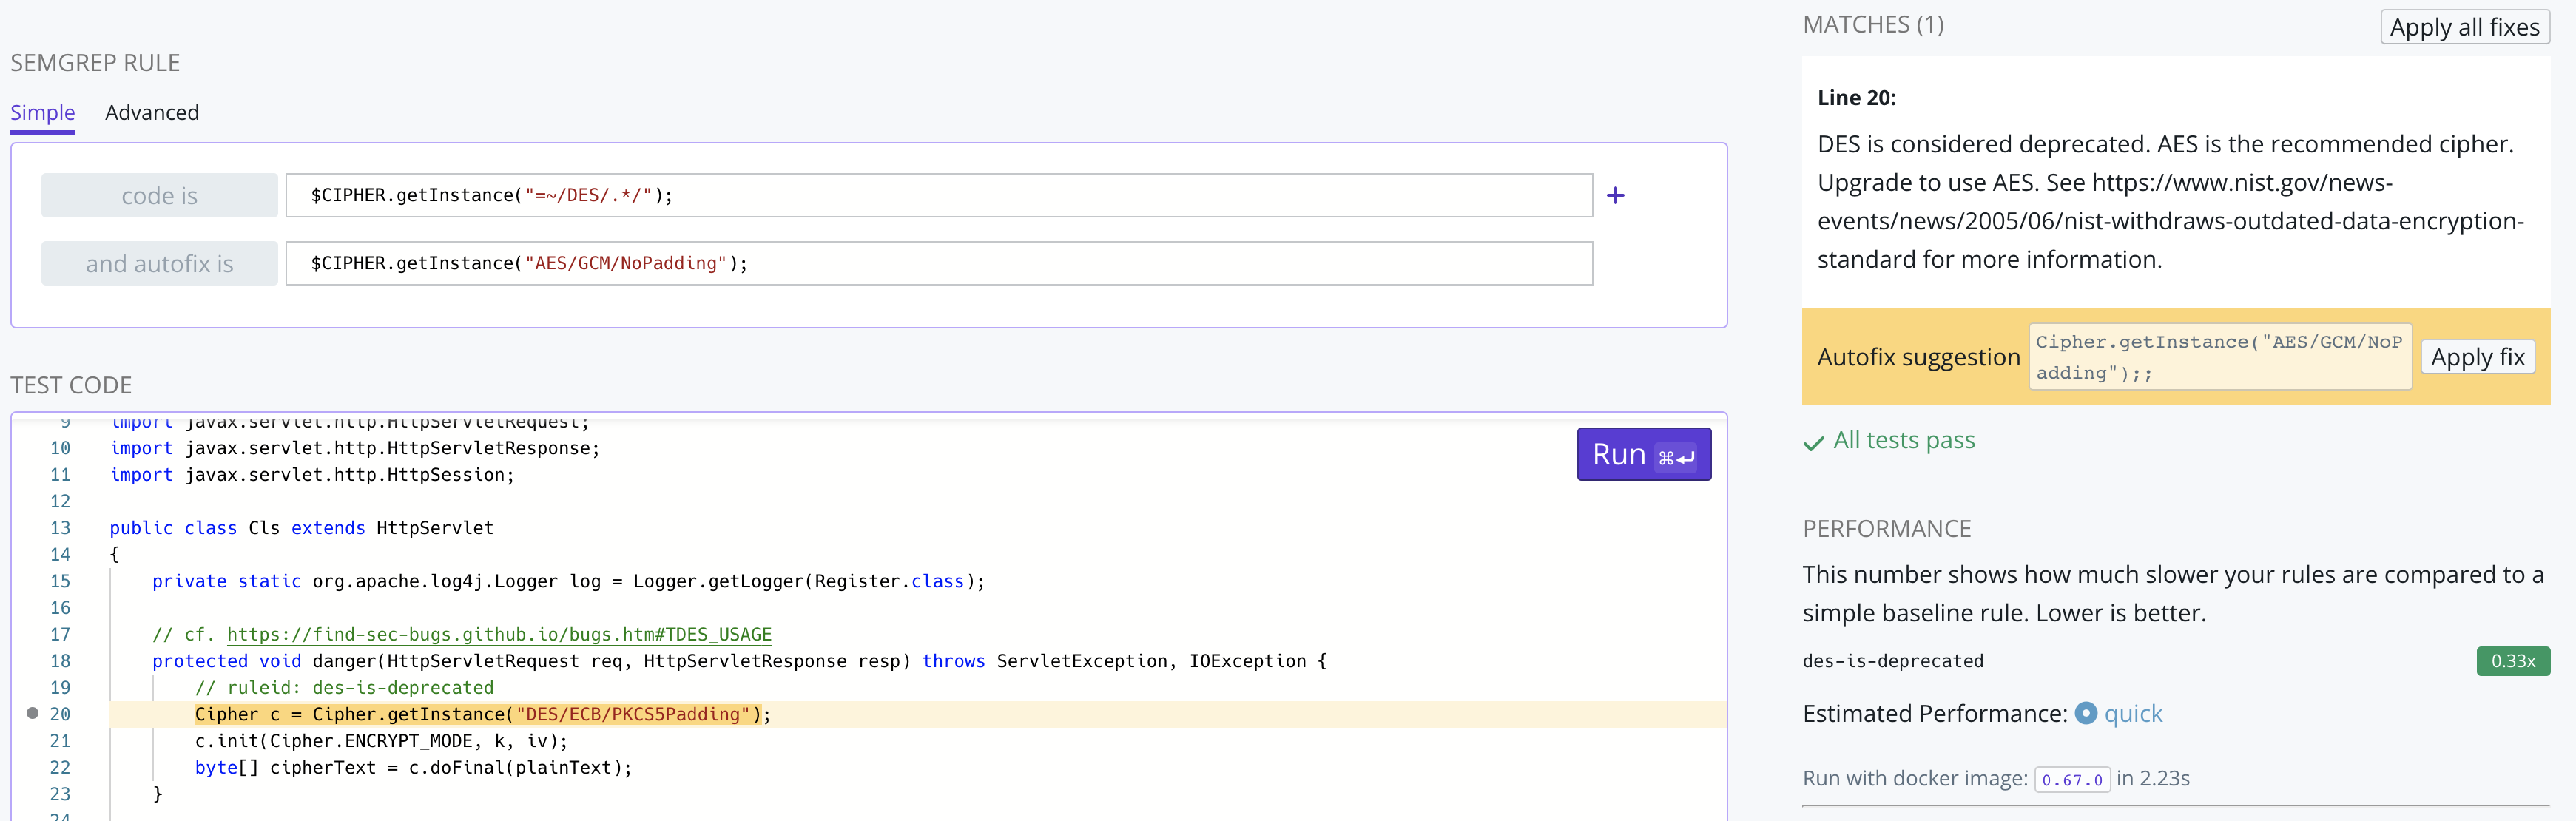
\includegraphics[width=\textwidth]{semgrep-editor.png}
  %\includegraphics[width=\textwidth,page=10]{04-tools/figures/figures2.pdf}
  \caption[Semgrep playground editor]{Semgrep's ``Simple" view in the Playground rule editor still requires use of the \gls{yaml} syntax.}
  \label{fig:semgrep-editor} 
\end{sidewaysfigure}

Semgrep also provides a few advanced features such as taint tracking which is similar to the concept of trusted input in Sensei.
To use taint tracking in a rule, sources and sinks need to be defined as well as optional sanitizers.
Since taint tracking requires a source to be specified, it functions differently to the trusted input of Sensei, where all input is untrusted by default.
Using metavariables it is possible to create a rule that prevents \glspl{efp} similarly to Sensei's trusted input. 
Listing~\ref{lst:metavariable} shows a rule to detect potential \gls{os} command injections, the analogous Sensei recipe is shown in Listing~\ref{lst:yamlrecipe}, but repeated here in Listing~\ref{lst:oscommand-sensei} for convenience.


\begin{minipage}[t]{0.9\linewidth}
\begin{lstlisting}[language={yaml},caption={Any commands passed on to the \texttt{exec} method that have not been retrieved through \texttt{getSafeCommand} will be marked.},label={lst:metavariable},xleftmargin=15pt]
rules:
- id: os-command
  patterns:
    - pattern: $RUNTIME.exec($COMMAND)
    - pattern-not-inside: |
        $COMMAND = getSafeCommand();
        ...
        $RUNTIME.exec($COMMAND);
  message: "Could lead to OS Command injection"
  languages: [java]
  severity: ERROR

\end{lstlisting}

\begin{lstlisting}[language={yaml},caption={Any input is untrusted by default except input retrieved through \texttt{getSafeCommand}. Untrusted input passed on to the \texttt{exec} methodcall will be marked.},label={lst:oscommand-sensei},xleftmargin=15pt]
search:
  methodcall:
    name: "exec"
    type: "java.lang.Runtime"
    args:
      1:
        type: "java.lang.String"
        containsUntrustedInput: true
        trustedSources:
        - methodcall:
            name: "getSafeCommand"
\end{lstlisting}
\end{minipage}
\section{Release and deploy}

High velocity of development and delivery is most easily achieved in \gls{saas} and other cloud computing delivery models.
It is easier to push frequent updates if there is only a single version of the application running, hosted centrally and managed by the software provider.
Furthermore, because the service provider has access to user data and behaviour, it is easier to collect feedback and make incremental improvements.
Finally, it is more economically viable to adapt to continuously changing requirements of customers, if the software is sold on a subscription basis.

\subsubsection{Infrastructure as code}
To keep pace with this high velocity of software development, new technology has been developed to automate infrastructure and deployment.
With \gls{iac}, the process of managing and provisioning data centers is done through machine-readable configuration files rather than hardware configurations and interactive tools~\cite{wittig2018amazon}.
Most frequently these configuration files are declarative, focusing on what the eventual target configuration should be, rather than describing the necessary changes to meet this configuration.
Two big components are required for automated infrastructure, those are application deployment and runtime orchestration.

\paragraph{Application deployment}
Modern software applications often consists of a variety of services, such as an \gls{api}, a web front-end, a back-end application, logging services, and services used for data analytics.
To ease the deployment, and to isolate services from each other, virtualization is used.
In early virtualization, a \gls{vmi} was created that contains the service's code and any requirements to run it, such as the \gls{os} and the dependencies.
A \gls{vmi} is a from of hardware virtualization, each is deployed as \textit{guests} on a \textit{host} machine, providing its own \gls{os} with its own kernel.
Because of this, \glspl{vm} can be deployed anywhere without requiring modifications.
This also has the added benefit of isolation between different services, so that each one has a fixed amount of \gls{cpu} processing power and memory.
However, they are large and take a lot of resources to store and run.

More modern technology moves from hardware virtualization to \gls{os}-level virtualization.
Here, the kernel of the host \gls{os} allows the existence of multiple isolated user space instances, called containers.
The most popular container technology today is Docker\footurl{https://www.docker.com/}.
With docker the application and its dependencies ara packaged in a virtual container that can run on any \gls{os}.
Docker containers are more lightweight, and a single server or \gls{vm} can run several containers simultaneously.
A docker container image is built by reading instructions from a Dockerfile\footurl{https://docs.docker.com/engine/reference/builder/}.
This file contains a selection of commands that a user could call on the command line interface to assemble the image.
An example of a Dockerfile is shown in Listing~\ref{lst:Dockerfile}.
The image is built from an ubuntu docker image. Then the contents from the \texttt{app} directory are copied to the image and the application is built using the make command. Finally the app is started.
Containers make it easy to control data and software components and make frequent updates such as security patches.

\begin{lstlisting}[language={Dockerfile},caption={Example of a Dockerfile to build and run a Python application.},label={lst:Dockerfile},xleftmargin=15pt]
# syntax=docker/dockerfile:1
FROM ubuntu:18.04
COPY . /app
RUN make /app
CMD python /app/app.py
\end{lstlisting}

Docker promotes the use of multi-container applications, where each service in the application is placed in its own container.
This is done through a docker-compose file, as shown in Listing~\ref{lst:dockercompose}.
This example, used during my research, sets up a mariaDB database and exposes it on port 3306. It also creates a web interface called Adminer, hosted on port 8080.

Placing separate services in their own containers like this, improves security, as containers, by default, run in isolation.
Each container can only access ports and files of other containers that are explicitly exposed by the other containers.

\begin{minipage}[t]{0.9\linewidth}
\begin{lstlisting}[language={YAML},caption={Example of a Dockerfile to build and run a Python application.},label={lst:dockercompose},xleftmargin=15pt]
version: '3.1'
services:
  maria:
    image: mariadb
    ports:
      - 3306:3306
    volumes:
      - mariadb:/var/lib/mysql
  web:
    image: adminer
    ports:
      - 8080:8080
volumes:
  mariadb:

\end{lstlisting}
\end{minipage}

Docker increases the level of security in comparison to running applications directly on the host.
It has features to more easily encrypt volumes, manage secrets, and encrypt communication between containers, all helping to avoid some of the top categories in the \gls{owasp} top 10.
But some misconfigurations can still downgrade the level of security and even introduce new vulnerabilities.
Many guides and training exist to help secure Dockerfiles and other container technology, including on the \gls{scw} portal, the \gls{owasp} website\footurl{https://cheatsheetseries.owasp.org/cheatsheets/Docker_Security_Cheat_Sheet.html}, and even \gls{nist}\footurl{https://csrc.nist.gov/publications/detail/nistir/8176/final}.
Some security tools, like Snyk, have adapted to scan for container misconfigurations, to detect, for example, use of containers with known vulnerabilities.

\paragraph{Runtime orchestration}
With runtime orchestration, the management of multiple physical servers is being abstracted as well.
An orchestration framework exposes a server cluster as if it were a single pool of resources, and allows the installation and management of containers across these servers from one centralized host.
Several runtime orchestration frameworks exist, with the most popular being Kubernetes (K8s), originally designed by Google and now maintained by the 
\gls{cncf}.
Runtime orchestration makes it easy to apply security practices such as network encryption, authentication, and management of application secrets\footurl{https://kubernetes.io/docs/concepts/security/overview/}. 

Kubernetes is designed to be highly customizable and developers must turn on certain features to make sure the resulting configuration is secure.
More information can be found on the \gls{owasp} website\footurl{https://cheatsheetseries.owasp.org/cheatsheets/Kubernetes_Security_Cheat_Sheet.html}.

\subsubsection{Policy as code}
With policy as code, isolation and decoupling is taken one step further.
A separate service is deployed that can be queried to make policy decisions.
One framework to run such a service is \gls{opa}, backed up be \gls{cncf}.

As an example, take a look at authorization decisions.
In a budgeting application, manager may be able to access the salary of anyone who reports to them.
To make such decisions, the management chain can be stored in the policy agent, an example is shown how this can be stored in \gls{opa} in Listing~\ref{lst:mgmt-chain}.

\begin{lstlisting}[language={json},caption={Management chain data example for use in OPA.},label={lst:mgmt-chain},xleftmargin=15pt]
{
    "management_chain": {
        "colin": [
            "pieter",
            "downey"
        ],
        "alex": [
            "gillis"
        ]
    }
}
\end{lstlisting}

It is then possible to define rules and execute queries based on this data.
In Listing~\ref{lst:opa-rule} rules are shown for the salary example.
Users are allowed to see their own salary and that of other users below them in the management chain.


\begin{minipage}[t]{0.9\linewidth}
\begin{lstlisting}[language={json},caption={OPA rules that define who has access to the salary of other users.},label={lst:opa-rule},xleftmargin=15pt]
default allow = false

allow {
    input.method = "GET"
    input.path = ["salary", id]
    input.user_id = id
}

allow {
    input.method = "GET"
    input.path = ["salary", id]
    managers = data.management_chain[id]
    input.user_id = managers[_]
}
\end{lstlisting}
\end{minipage}

The budgeting application can then make decisions by querying the \gls{opa} service as shown in Listing~\ref{lst:opa-query}.

\begin{minipage}[t]{0.9\linewidth}
\begin{lstlisting}[language={java},caption={Management chain data example for use in OPA.},label={lst:opa-query},xleftmargin=15pt]
> input := {"method": "GET", "path": ["salary", "colin"], "user_id": "gillis"}
> allow
false
\end{lstlisting}
\end{minipage}

Decoupling policy decisions like this has many advantages.
It provides a centralized overview of policies and avoids redundancy in implementations.
In another application, for example, employees are able to request absence and these requests can be authorized by their manager.
Instead of implementing these decisions again in the second application and possibly even storing the data multiple times, the \gls{opa} service can be reused by adding new rules.

Because of the declarative nature of the rules, they can be understood easily, causing reduced complexity and hence reduced chance for mistakes.
The policy agent can be used to overcome several vulnerabilities in \gls{owasp} top 10, such as authentication and authorization decisions, as well as some business logic flaws.

By using a policy as code service, logging of the policy decisions will also be done separately from application logs.
This can make it easier to monitor and detect abnormal usage of the application, partly mitigating the security problem of excessive logging in the application itself.

%
%\paragraph{CodeInspector}
%%%https://www.code-inspector.com/

%\paragraph{Pluralsight}
%%https://help.pluralsight.com/help/vs-code-extension
%
%\paragraph{RuleGuard}
%
%\paragraph{Explore.dev}
%%https://explore.dev/
%
%\paragraph{Deepcode}
%(Matias:)
%deepcode.ai
%Deepcode is a University project spin off (Spun of in 2016). It’s focus was on quality code, not security in specific.
%Focus on:
%* Accuracy
%* Speed
%* For developers
%When demoing, main focus went to the IDE plugin (Can also work in Pull request and in CD/CD). Demo was very slick. it shows errors and warnings, and it shows other places in the code where a developer made that change before, essentially they went through the entire history of checkins and make rules out of that (not really rules, it is in their AI/ML module). So it is not only finding, it does have a focus on real fixes, potentially in line with the code base, stuff that can actually work.
%AI/ML component is very interesting. AI/ML instead of rules based is very interesting. If this works, if they can pull that off, it is a good approach to get rid of manual effort and still be custom to the code (but that is not the focus, so this is not happening right now). It diminishes the number of researchers they have to have on staff to create rules. It reduces the time to value for customers using the solution.
%Compared to Semmle: Seems to have a lot of similarities. Started as a tool focused on quality, not specifically security. Was a university project first which was incubated, so not really a focus on making this work at scale. (Great for a demo, great in theory, great on a small code base, but what about the real world). However, from what they have shown, it looks better/easier/slicker/more mature than Semmle.
%If the demo works in practice on large codebases, then I think it will be a significant challenger for the established SAST solutions.
%I think there is an opportunity for SCW to be in there and educate the developer. The examples in the demo were simplistic (hardcoded passwords) so there was no need for training, but I can see a role for the SCW training platform with what I’ve seen
%Sensei, that becomes more interesting, but there are advantages and disadvantages. Sensei is still real-time, Snyk Code is when pressing a button, and in a different window. Sensei has a quick fix, Snyk does not have one. Sensei is more tailored to the code, Snyk is not. But then there are undeniable advantages of their approach. The ML/AI instead of rules should be better in terms of configuration, rules support, … if and only if this AI/ML thing work. And that AI/ML thing may show quicker value than Sensei, as the upfront work is less on Snyk code. Sensei feels more enterprise than Snyk code tbh, I don’t see them doing what we do at NetSuite, that AI/ML is too free form and can propose whatever.
%
%(Brysen:)
%I just watched the demo videos on their youtube channel.
%Sending your code to their servers is an annoying thing.
%The way they provide a “fix” is done by showing you examples of open source repos where this issue should have been fixed, but in their example it doesn’t even show the same code as the found vulnerability so effectively the user still needs to plow through the suggested changes and determine if they are right in which they still need a good too strong security knowledge.
%
%Specifically to Sensei, one thing we have to copy is showing an example. So the suggestion they make is together with an example of another place in the code where this is also the case (or where that same change was executed). That looked really cool. I think in Sensei that would work even better, because we should do that in the code base itself, and not on some random other open source project... My 2 cents

%\subsubsection{SecureAssist}
%SecureAssist~\cite{secureassist} is an IDE plugin targeting the discovery of security bugs in code. It is available for eclipse, intelliJ, VisualStudio, RAD, and Spring Tool Suite~\cite{sastinide}. Its scans are not in the IDE but on the enterprise portal. The results are sent back to the IDE once completed. This allows scanning without preventing the developer from continuing his work, which contrasts with the Fortify Security Assistant, that prevents developers from changing the code during a scan. Remediation is provided in the form of descriptions that explain the attack and provide some code examples but the tool does not provide quick fixes~\cite{secureassistide}. 
%
%Rule packs are distributed as JAR files and the tool provides a Rulepack Configurator similar to Sensei's cookbook Manager.

%\subsubsection{Aside}
%The OWASP ASIDE/ESIDE~\cite{aside} project consist of two branches, the ASIDE branch that focuses on detecting software vulnerabilities and helping developer write secure code, and the ESIDE branch that focuses on helping students in acquiring secure programming knowledge and practices.
%
%Application Security IDE (\emph{ASIDE}) performs fast scans of the code in Eclipse, but unlike Sensei the scans need to be started manually. Besides detecting vulnerabilities they also provide quick fixes for some issues. The quick fixes require the developers to choose from a list of options, which could overwhelm them. In previous research a large number of false positives were detected~\cite{xie2011aside}, however, most of these are what is considered protection for future use in this paper. They are cases where best practices should be applied even if their violation is not yet exploitable at this point in development. They also mark variables in the code that are tainted, this could be compared to Sensei's concept of untrusted input. Untrusted input in Sensei is not currently marked to avoid unnecessary clutter. 
%
%The goal of ESIDE~\cite{eside,whitney2018embedding} is to provide information and training at all times during the education. Its rules can not be configured and the tool does not provide quickfixes. However they provide explanation in external web pages linked from Eclipse. Their information is similar to our full coding guidelines where information on APIs and a correct code example is provided. 
%
%
%
%
%
%
%